\documentclass{ou-report}

\citestyle{agu}
\usepackage{float}

% Dit template is gemaakt door P.J. Molijn in het kader van zijn afstuderen aan de OU in 2014.
% Waarvoor hartelijk dank.
% Minieme maar belangrijke wijzigingen zijn aangebracht door E.M. van Doorn
% Het template is versimpeld door Sylvia Stuurman, 2019.

\makenoidxglossaries

\newacronym{gw}{GW}{Gravitational Waves}
\newacronym{bbh}{BBH}{Binary Black Hole}
\newacronym{ns}{NS}{Neutron Star}
\newacronym{bns}{BNS}{Binary Neutron Star}
\newacronym{cbc}{CBC}{Compact Binary Coalescence}
\newacronym{ligo}{LIGO}{Laser Interferometer Gravitational-wave observatory}
\newacronym{o1}{O1}{First observing run}
\newacronym{o2}{O2}{Second observing run}
\newacronym{o3}{O3}{Third observing run}
\newacronym{nsbh}{NSBH}{Neutron Star-Black Hole}
\newacronym{ccsne}{CCSNe}{Core-Collapse Supernovae}
\newacronym{dl}{DL}{Deep Learning}
\newacronym{ml}{ML}{Machine Learning}
\newacronym{ai}{AI}{Artificial Intelligence}
\newacronym{cnn}{CNN}{Convolutional Neural Network}
\newacronym{fd}{FD}{Fractal Dimension}
\newacronym{idq}{iDQ}{inferential Data Quality}
\newacronym{pca}{PCA}{Principal Component Analysis}
\newacronym{svm}{SVM}{Support Vector Machine}
\newacronym{lr}{LR}{Logistic Regression}
\newacronym{xgb}{XGBoost}{Extreme Gradient Boosting}
\newacronym{gwosc}{GWOSC}{Gravitational-wave Open Science Center}
\newacronym{snr}{SNR}{Signal-to-Noise Ratio}
\newacronym{od}{OD}{Object Detection}
\newacronym{yolo}{YOLO}{You Only Look Once}
\newacronym{map}{mAP}{mean Average Precision}
\newacronym{var}{VAR}{Variation method}
\newacronym{anam}{ANAM}{Averaged Normalized Autocorrelation Method}
\newacronym{il}{IL}{Incremental Learning}
\newacronym{xdg}{XdG}{Context-dependent Gating}
\newacronym{ewc}{EWC}{Elastic Weight Consolidation}
\newacronym{si}{SI}{Synaptic Intelligence}
\newacronym{lwf}{LwF}{Learning without Forgetting}
\newacronym{fromp}{FROMP}{Functional Regularization Of the Memorable Past}
\newacronym{dgr}{DGR}{Deep Generative Replay}
\newacronym{bir}{BI-R}{Brain-Inspired Replay}
\newacronym{er}{ER}{Experience Replay}
\newacronym{agem}{A-GEM}{Averaged Gradient Episodic Memory}
\newacronym{gem}{GEM}{Gradient Episodic Memory}
\newacronym{cl}{CL}{Continual Learning}
\newacronym{sgd}{SGD}{Stochastic Gradient Descent}
\newacronym{scr}{SCR}{Supervised Contrastive Replay}
\newacronym{ncm}{NCM}{Nearest-Class-Mean}
\newacronym{der}{DER}{Dark Experience Replay}
\newacronym{der++}{DER++}{Dark Experience Replay ++}
\newacronym{umap}{UMAP}{Uniform Manifold Approximation and Projection}
\newacronym{tsne}{t-SNE}{t-Distributed Stochastic Neighbor Embedding}

\begin{document}
\pagestyle{plain}
\title{Enhancing Glitch Identification in Gravitational Wave Analysis: A Continual Learning Approach}
\author{Brian Baert}

\begin{titlepage}

\begin{center}

%% Insert the OU logo at the bottom of the page.
\begin{tikzpicture}[remember picture,overlay]
    \node at (current page.south)[anchor=south,inner sep=0pt]{
%        \includegraphics[scale=0.7]{cover/logo}
    };
\end{tikzpicture}

%% Extra whitespace at the top.
\vspace*{2\bigskipamount}

%% Print the title in specific color.
{\makeatletter
%\titlestyle\color{ou-cyan}\Huge\@title
\titlestyle\color{red}\Huge\@title
\makeatother}

%% Print the optional subtitle in black.
{\makeatletter
\ifx\@subtitle\undefined\else
    \bigskip
    \titlefont\titleshape\LARGE\@subtitle
\fi
\makeatother}

\bigskip
\bigskip

by
%door

\bigskip
\bigskip

%% Print the name of the author.
{\makeatletter
\titlefont\Large\bfseries\@author
\makeatother}

\vfill

in partial fulfillment of the requirements for the degree of
%in overeenstemming met de vereisten voor het verkrijgen van de graad van

\bigskip
\bigskip

{\bfseries Master of Science}

in Artificial Intelligence

\bigskip
\bigskip

at the Open University, Faculty of Science \\
Master Artificial Intelligence
%aan de Open Universiteit Nederland,

to be defended publicly on Day Month DD, 2024 at HH:00 PM.
%in het openbaar te verdedigen op dinsdag 9 september om 15:00 uur.

\vfill

\begin{tabular}{lll}
%% Add additional information here, per faculty requirements, e.g
    Student number: & 850794710 \\
    Course code: & IM9506 \\
    Thesis committee:
        & Dr. Stefano Bromuri (chairman), & Open University \\
        & Dr. Daniel Tan (supervisor), & Open University
\end{tabular}

%% Only include the following lines if confidentiality is applicable.
\bigskip


\bigskip

\end{center}

\end{titlepage} 

\clearpage
\printglossary[type=\acronymtype]
\printnoidxglossaries
\clearpage

\pagenumbering{roman}

\frontmatter 


\let\cleardoublepage\clearpage

% Optional Dedication, Acknowledgement
%\input{dedication}

%\section*{Acknowledgement}
Embarking on this journey into the fascinating field of Continual Learning and Glitch Detection would not have been possible without the support of many incredible people. \\

First and foremost, I want to express my gratitude to my supervisors, Dr. Stefano Bromuri and Dr. Daniel Tan as well as Tom Dooney. Your guidance and insightful discussions, and unwavering patience throughout this process were invaluable. \\

My heartfelt thanks go to the entire faculty and staff at Howest (Howest University of Applied Sciences). My homebase and supportive environment. A special shout-out to the Applied Computer Science education program for their tireless efforts to aid me wherever they could, especially the program coordinator, William Schokkelé, Director of Education, Isabel Uitdebroeck and my dear colleague Dr. Ines Devlieger for her critical eye on proofreading the results section. \\

To my amazing husband, Cédric, my unwavering rock throughout this endeavor, thank you for your belief in me. Your understanding during late nights and weekends spent buried in research has been a source of immense strenght. I would not be here without your support and love.\\

Who would have thought that at the age of 41 I would finally succeed in achieving one of my long aspired goals of achieving a Master of Science degree, a journey that started over three years ago with a Postgraduate has finally come to an end. An open ending because life starts at 41 right...\\


\tableofcontents

%Optional: list of figures, list of tables
%\listoffigures

%\listoftables

%% Include an optional summary page.
%\input{Summary/summary}
%\input{Summary/samenvatting}

\mainmatter
\pagenumbering{arabic}

\chapter{Introduction}
\label{ch:1}
\section{Introduction}
\label{sec-Introduction}
The following thesis investigates \acrlong{cl} as a framework for robust and efficient \acrlong{gw} analysis. \acrshort{cl} algorithms excel at incrementally learning from new data streams while retaining knowledge of previously encountered classes \citep{van2022three, qu2021recent, de2021continual}.\\
\acrshort{gw} are ripples in space-time caused by violent disruptions in the universe. Massive accelerating objects like \acrlong{ns} (\acrshort{ns}) and \acrlong{bbh} (\acrshort{bbh}) cause such strong waves propagating in all directions. Other cataclysmic events, responsible for \acrshort{gw}, are supernovae and obviously residues of the Big Bang \citep{CaltechWhatAreGW}. \\
Although the generation of \acrshort{gw} is a frenzy of energy, by the time the waves (invisible for the human eye) reach earth they are imperceptibly small.\\
The birth of \acrshort{ligo} (\acrlong{ligo}) offered a way to make very small measurements, equivalent to fractional changes in distance of $10^{-21}$ (smaller than an atom), microscopic measurements needed to detect \acrshort{gw} \citep{zevin2017gravity,glanzer2023data}. \\
\acrshort{ligo} has already completed three observing runs, abbreviated \acrshort{o1} (\acrlong{o1}), \acrshort{o2} (\acrlong{o2}) and \acrshort{o3} (\acrlong{o3}). At this very moment of writing the fourth observing run started on May the 24th of 2023 and the first period, 04a has ended on January the 16th of 2024 \citep{LIGORunPlan}. \\
Up to this point the types of uncovered \acrshort{gw} signals are limited to \acrshort{bbh}, \acrlong{bns} (\acrshort{bns}) and \acrlong{nsbh} (\acrshort{nsbh}) incidents. Researchers hope to unravel previously unseen cosmological cataclysms such as \acrshort{ccsne} (\acrlong{ccsne}), magnetars or probabilistic background waves from the Big Bang \citep{cuoco2020enhancing}. \\
\acrshort{gw} Analysis is a challenging field where scientists with varying backgrounds work together. With each observing run of \acrshort{ligo} resulting in more detected gravitational events (the majority were \acrshort{bbh} mergers) \citep{zevin2017gravity,glanzer2023data}, \citep{CaltechFAQ}. 

The accurate identification of \acrshort{gw} signals amidst noisy data remains a significant challenge. One of the primary sources of noise in \acrshort{gw} detectors are glitches. 
Glitches are short-lived non-Gaussian noise features that can be instrumental or environmental in nature. Glitches impact the analysis of wave candidates in three ways. Firstly, glitches increase the background loudness and thus reduce the candidate significance. Secondly glitches increase the uncertainty in the categorisation process because they operate with the same amplitude of astrophysical signals. Thirdly, the amount of usable data is even decreased more due to glitch contamination \citep{zevin2017gravity, cuoco2020enhancing}. \\
\acrlong{dl} (\acrshort{dl}) and especially \acrlong{cnn} (\acrshort{cnn}) have proven to be suitable architectures for extracting glitch features \citep{george2017deep,glanzer2023data,fernandes2023convolutional}. Together with the GravitySpy citizen science project \citep{bahaadini2018machine, zevin2017gravity}, the images can then be classified into their corresponding glitch morphologies, as seen in Figure \ref{fig:glitch_morphologies}.

\acrshort{gw} detectors host hundreds of thousands of auxiliary channels that monitor the state of the instruments and the environment. They have shown promise in characterizing glitches, such as \acrlong{idq} (\acrshort{idq}) \citep{essick2020idq,davis2022detector} or Elastic-net based ML for Understanding (EMU) \citep{colgan2020efficient} have been studied. The fusion of \acrfull{fd} analysis and \acrshort{ml} offers a robust framework for glitch detection in \acrshort{gw} analysis. Moreover, the scalability of \acrshort{fd} analysis across auxiliary channels holds promise for real-time glitch detection \citep{colgan2020efficient, benedetto2023ai}.

The limitations of the current classical approaches of offline training a neural network are evident due to the new data expected to be delivered in the fourth observing run \citep{wu2024advancing}. In this context, the field of \acrfull{il} or \acrshort{cl} emerges as a compelling area. The \acrshort{il} approach offers a fresh framework that allows models to learn from a continuously expanding dataset while still maintaining performance on previously encountered data \citep{van2022three, qu2021recent, de2021continual}.
Unlike batch learning, where models are trained on static datasets, \acrshort{cl} enables models to adapt incrementally to new data while retaining knowledge of previously encountered classes \citep{kirkpatrick2017overcoming}. 

In the context of \acrshort{gw} analysis, \acrshort{cl} strategies allow us to accommodate new glitch classes (as \acrshort{ligo} continues to operate and collect data, new glitch classes may emerge where \acrshort{cl} ensures that the model can seamlessly incorporate these novel classes without compromising performance on existing ones). It mitigates catastrophic forgetting (traditional \acrshort{ml} models tend to forget previously learned information when exposed to new data. \acrshort{cl} methods such as \acrfull{ewc} or memory-augmented architectures address this issue by preserving knowledge of existing glitch morphologies \citep{abbott2023open, kirkpatrick2017overcoming}.  

\begin{figure}[H]
    \centering
    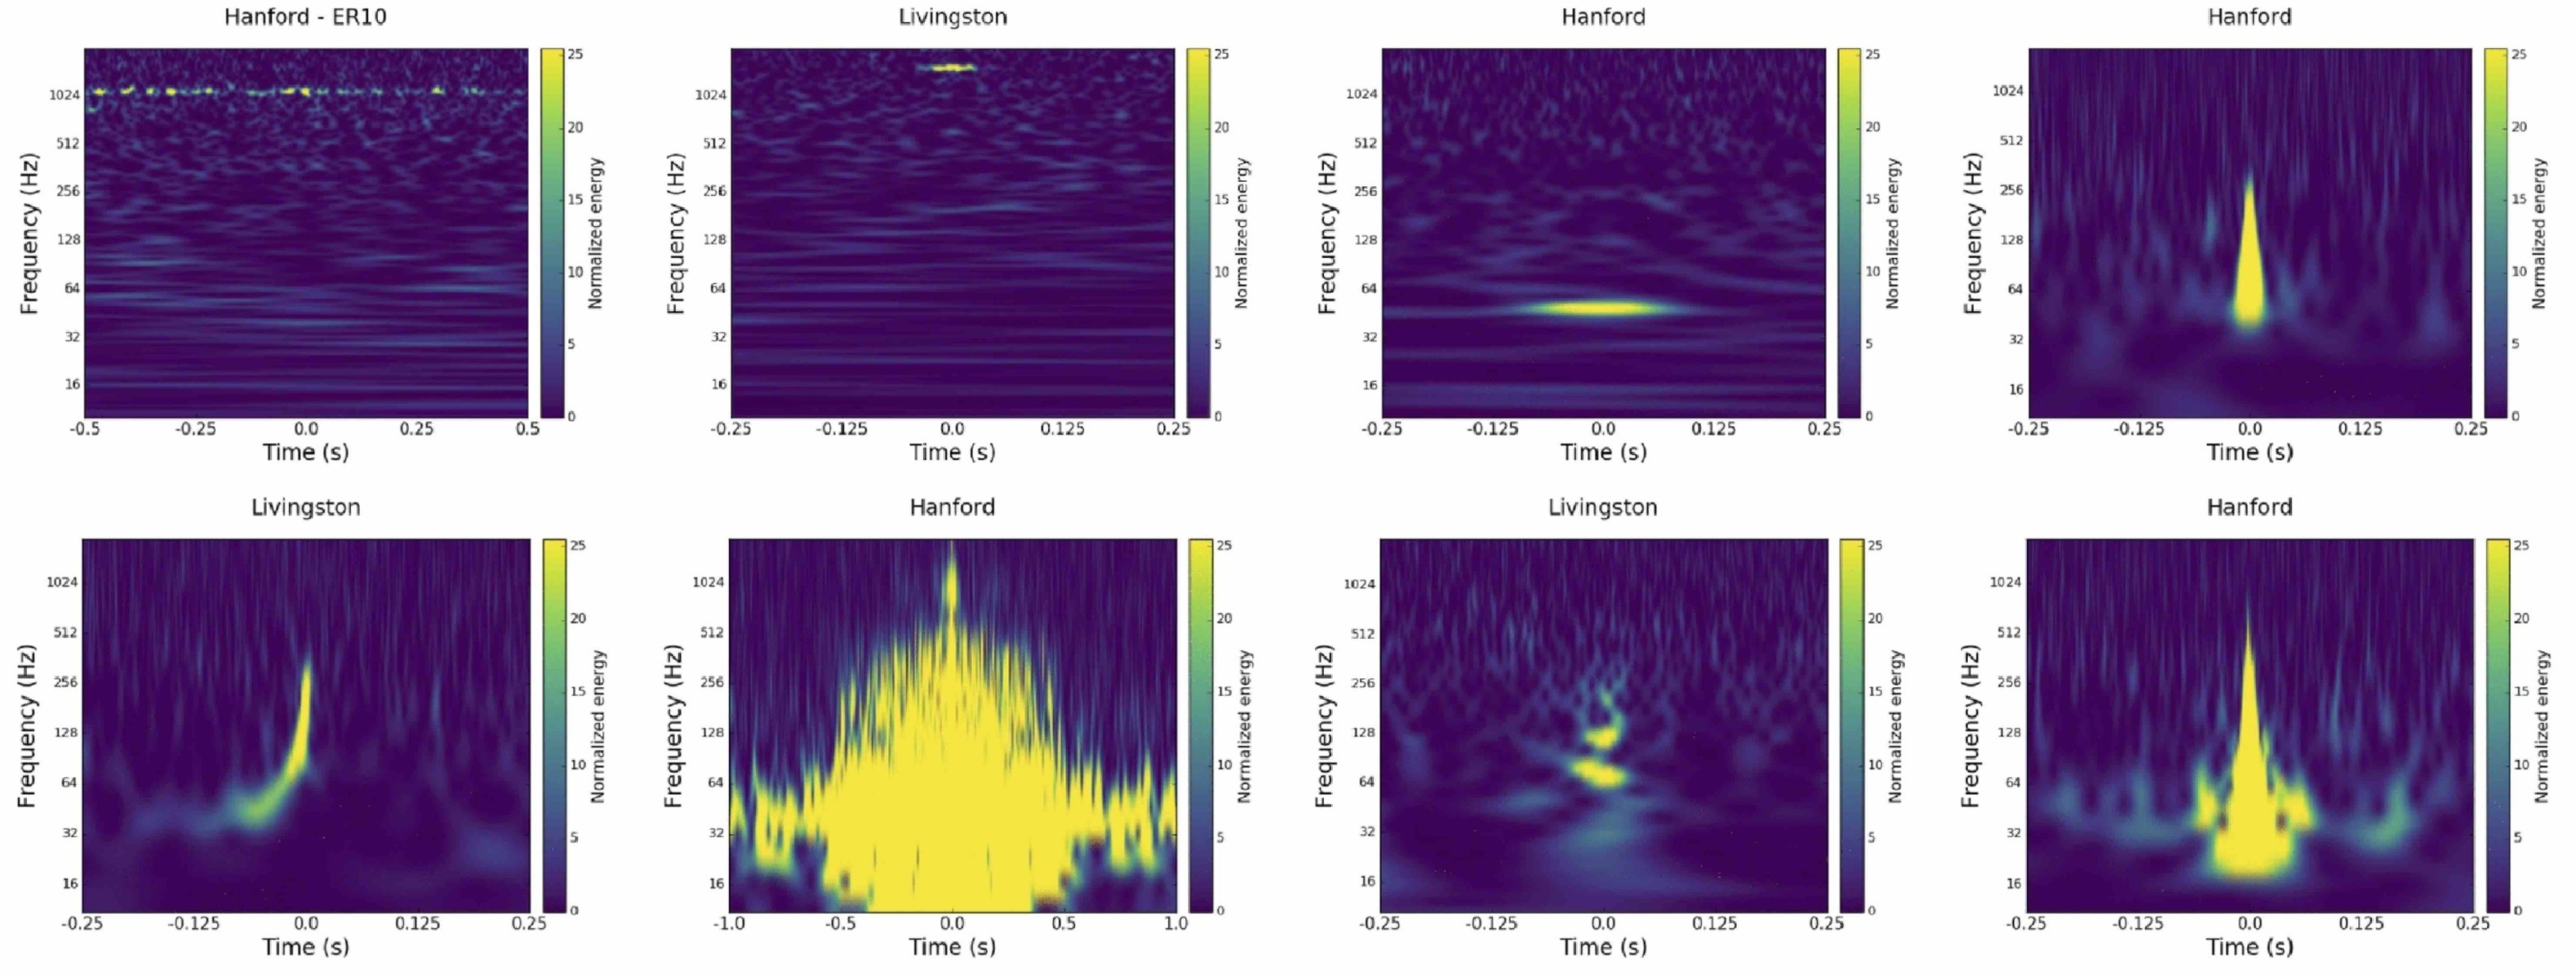
\includegraphics[width=0.8\textwidth]{Images/glitch_morphologies.jpg}
    \caption{Some glitch class morphologies. From top left to bottom right: 1080Lines, 1400Ripples, Air Compressor, Blip, row two: Chirp, Extremely Loud, Helix, Koi Fish. from \citep{glanzer2023data}}
    \label{fig:glitch_morphologies}
\end{figure}

In addition to identification and characterization of glitches, noise subtraction is another problem relating to signal processing \citep{benedetto2023ai, ormiston2020noise, davis2022detector, cornish2021bayeswave}. BayesWave is a tool that can be used to split the \acrshort{gw} signal from the noise \citep{cornish2021bayeswave}.

Glitches are only one side of the spectrum, it is evenly important that \acrlong{cbc} (\acrshort{cbc}) parameters can be correctly estimated. Researchers typically use waveform templates to compute the necessary parameter posteriors based on numerical solutions to the two body problem, but this remains computationally inefficient \citep{ajith2011addressing,coogan2022efficient,isoyama2020post}.

Searching GW signals is commonly split up in four separate categories. The first one being the \acrshort{cbc}'s (\acrshort{bbh}, \acrshort{bns}, \acrshort{nsbh}), the second type are called \acrshort{gw} bursts these can be the product of \acrshort{ccsne} or pulsar glitches. The third type are called long continuous \acrshort{gw}. The last category are residue waves from distant \acrshort{cbc}'s or even the Big Bang
\citep{abbott2020guide, LIGO_continuous}. The use of \acrlong{ml} (\acrshort{ml}), especially Random Forests (RF) was able to increase the detection speed of \acrshort{cbc}'s \citep{kapadia2017classifier}. The \acrlong{dl} (\acrshort{dl}) approach on the other hand has had mixed results \citep{gebhard2019convolutional,chatterjee2021extraction,ruan2023rapid}. 
Searching for other types of signals via \acrshort{ml} or \acrshort{dl} remains difficult because there is much uncertainty about morphology (due to lack of training data) \citep{cuoco2020enhancing}. 

A last application area where \acrshort{dl} is being investigated is the estimation of astrophysical parameters. Here Bayesian approaches have the ability to proof usefull, but the computational cost of calculating all posterior probabilities is an obstacle \citep{cuoco2020enhancing}.

\section{Thesis structure}
The thesis is structr
\newpage





\chapter{Related work and Background}
\label{ch-2}
\section{Related work}
\subsection{Gravity Spy}
The construction of one of the main datasets for the classification and detection of glitches is the Gravity Spy dataset \citep{zevin2017gravity, glanzer2023data}. 
The Gravity Spy dataset consists of a large set of Qscans (also called spectrograms). These Qscans are obtained via the Omicron algorithm pipeline \citep{robinet2020omicron}. Omicron originates from the Q-transformation \citep{chatterji2004multiresolution}. The colour scale, or normalized energy, used in these images, as in Figure \ref{fig:spectrogram_examples}, is the square of the \acrshort{snr} in a given Q-tile, divided by the mean squared magnitude for stationary white noise.
\begin{figure}[H]
    \centering
    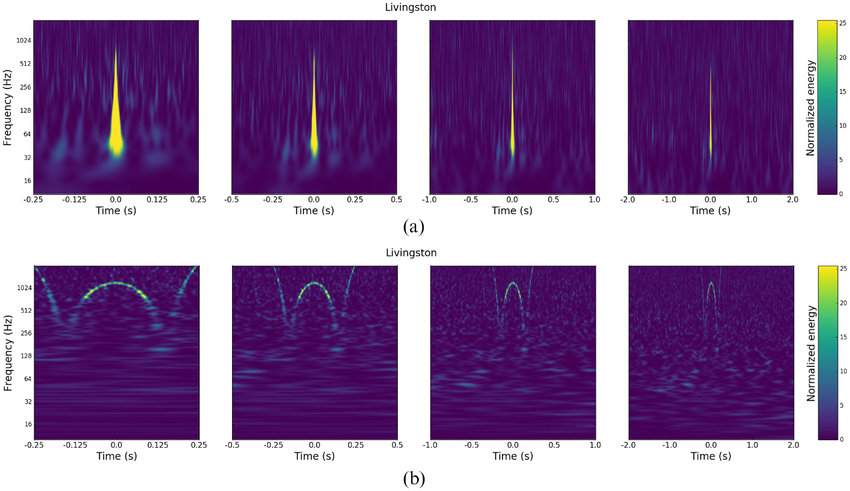
\includegraphics[width=0.8\textwidth]{Images/omegascan_examples.jpg}
    \caption{\acrshort{ligo} Qscan images of 'blip' (first row) and 'whistle' (second row) over four different durations \citep{zevin2017gravity}}
    \label{fig:spectrogram_examples}
\end{figure}
The researchers use visual inspection by citizen scientists as well as \acrshort{dl} classification using a \acrshort{cnn}. The \acrshort{cnn} outputs a confidence score $p$ for each glitch class by using a softmax layer. \\

\subsection{Glitch classification}
Because the \acrshort{gw} signal strength is weaker than the background noise, the preferred architecture is often a \acrshort{cnn}'s with wavelet and Q-transforms \cite{cuoco2020enhancing}. 

The proposed \acrshort{dl} methodology presented in \citep{bicskin2023fast} uses a combination of \acrshort{ml} and \acrshort{dl} algorithms for classification. It consists of two phases, first, they utilise feature extraction possibilities of the pre-trained \acrshort{dl} models Inception-v3 \citep{szegedy2016rethinking} and ResNet-50 \citep{he2016deep} on the Q-transformed glitch images. Secondly, they apply \acrshort{pca} to select 100 components, these serve as input for \acrshort{svm}, \acrshort{lr} and \acrshort{xgb} algorithms. They opted to use only 10 glitch classes from the Gravity Spy dataset and no up- or downsampling techniques to issue the imbalancedness of the dataset. All samples are Q-transformed before entering the training phase. The results showed that Inception-v3-based architectures perform faster and the \acrshort{lr} algorithm delivers the highest accuracy on the test set ($96.06$\%). Certain glitch morphologies like '1400 ripples', 'light modulation', 'Tomte' and 'None of the above' had substantially lower scores.

The usage of \acrshort{cnn} for glitch classification is described in \citep{fernandes2023convolutional}. They opt for a ResNet \citep{he2016deep} architecture baseline (ResNet18 and ResNet34) and the \verb|fastai| \verb|fit_one_cycle| route. 

\subsection{GW detection}
The updated Gravity Spy classification model \citep{jarov2023new} can differentiate \acrshort{cbc} signals from detector glitches. To achieve this accuracy improvement, they used a two-step approach. First, a baseline segment is selected from \acrshort{o3} and the \verb|pycbc| package \citep{nitz2020gwastro} is used to inject waveform simulations originating from masses between $3M_{\odot}$ and $350M_{\odot}$. Secondly, two classifiers (one for low-mass signals and one for high-mass \acrshort{cbc} signals) are implemented. Because certain glitch morphologies have similar structures, this type of noise must be inserted in the training set as well. Finally, the Gravity Spy CNN architecture is retrained on the extended training sets resulting in a signal-versus-glitch classifier. The relationship between the total mass of the inspiraling objects and the \acrshort{gw} accuracy was the main reason for splitting the classifiers into low and high masses. 
\subsection{Object detection for CBC}
\begin{wrapfigure}{r}{5cm}
    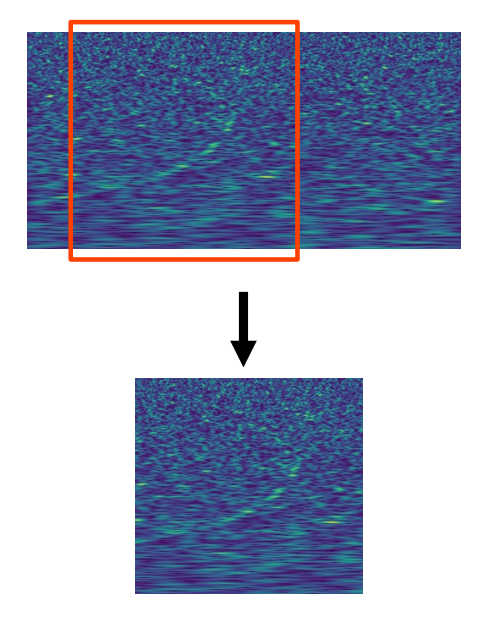
\includegraphics[width=0.25\textwidth]{Images/od_bns.png}
    \caption{Qscan generation and final 8-bit PNG image \citep{aveiro2022identification}}
    \label{fig:od_bns}
\end{wrapfigure}
Researchers \citep{aveiro2022identification} have investigated the use of a classical single shot \acrlong{od} method, \acrfull{yolo} \citep{redmon2016you}, to detect a subset of \acrshort{cbc} events, namely \acrshort{bns} mergers. Single shot detector methods are cost- and time-efficient \citep{redmon2017yolo9000} and hence are suitable candidates to integrate in a \acrshort{cbc} object detection method. 
They use generated \acrshort{bns} signals via the \verb|PyCBC| package \citep{nitz2020gwastro} and the generation pipeline from \citep{gebhard2019convolutional}. The generated signals are then randomly cut to the required 8s duration, with one condition, the generated waveform must be in the cut. 
Just as in the Gravity Spy generation process \citep{zevin2017gravity}, the Q-transform \citep{chatterji2004multiresolution} is used to generate the Qscans (here they opt for the \verb|librosa| package \citep{mcfee2015librosa}). 

The Qscans are converted to 8-bit PNG images as seen in Figure \ref{fig:od_bns}

The bounding box coordinates of the \acrshort{gw} class are included in a separate text file per image. Labelling is automated as part of the generation pipeline. Initial tests were promising with acceptable \acrfull{map} results. The research team experimented with varying \acrshort{snr} parameters (between 10 and 20). Lower \acrshort{snr} degraded the resulting metrics. Although no real training data were used, exploratory tests on GW170817 \citep{abbott2017gw170817} and GW190425 \citep{abbott2020gw190425} \acrshort{bns} coalescence events indicate the model's ability to perform \acrshort{gw} detections.



\subsection{Fractal based noise characterisation}
Two relevant studies were \citep{cavaglia2022characterization} and \citep{laguarta2023detection}. The noise found in \acrshort{gw} detectors usually is non-Gaussian and non-stationary \citep{abbott2020guide}. Distinguishing noise from spectrograms and auxiliary channels can be done straightforwardly, but determining the \acrshort{cbc} parameters is not \citep{powell2018parameter}. Researchers \citep{cavaglia2022characterization} propose utilising \acrfull{fd} on auxiliary channels like instrumental control data to identify transient origins of noise. \acrshort{fd} calculation approximations are done in a time-efficient way. Fractals are basically subsets of $n$-dimensional Euclidean spaces \citep{mandelbrot1989fractal} where $D_{F} < n$ and $D_{F} \not\in \mathbf{Z}$. \acrshort{fd} measures the degree of complexity of the set. The Minkowski-Bouligand or box-counting definition is used \citep{weisstein2019minkowski}. The definition used in \citep{cavaglia2022characterization} is taken from \citep{dubuc1989evaluating}. 
Because exact measurements are not uniformly defined, approximations like \acrfull{var} or \acrfull{anam} are used.\citep{cavaglia2022characterization} prefers the \acrshort{var} approximation and applies it to two stretches of \acrshort{ligo} data from \acrshort{o3} where whistle glitches occur. Whistle glitches are short-duration noise (around 1 second) and have a frequency between 100Hz and several kHz.  In the analysis, the focus lies on the strain data and only one auxiliary channel \verb|L1:LSC-PRCL_OUT_DQ| (interferometer PRC (Power Recycling Cavity) monitor). 
\begin{figure}[H]
    \centering
    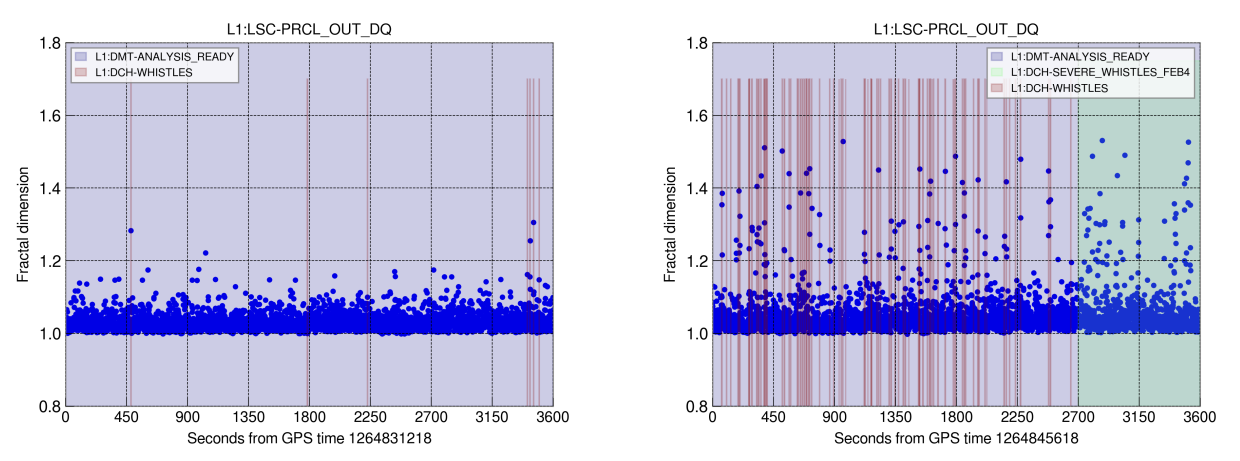
\includegraphics[width=0.9\textwidth]{Images/fd_L1_LSC_PRCL_OUT_DQ.png}
    \caption{\acrshort{fd} plot for the L1:LSC-PRCL\_OUT\_DQ auxiliary witness channel. On the left plot nominal interferometer observing mode. On the right plot data with a growing rate of glitches. \citep{cavaglia2022characterization} }
    \label{fig:fd_L1_LSC_PRCL}
\end{figure}
In the left plot of Figure \ref{fig:fd_L1_LSC_PRCL} it is clear that the nominal \acrshort{fd} is static and $D_{F}$ ranges between 1 and 1.2. Investigating the Q-scans of the noise points with $D_{F} > 1.2$ shows, at least for three out of four points, a clear whistle signal is diagnosed. In the right plot a big amount of noisy glitches is shown, this renders the data unusable for \acrshort{gw} analysis. Their experiment was done on another data strain, showing similar results. They conclude that \acrshort{fd} can be used to investigate the stationarity (or non-) of the interferometer in the company of noise.  Periods with a lot of (high) frequency noise show an increase in \acrshort{fd} variability \citep{cavaglia2022characterization}.

Researchers \citep{laguarta2023detection} use a convolutional autoencoder approach to cope with the absence of a ground truth and the absence of absolute order (variety of magnitudes). Although there are many studies on glitch morphologies, we are not sure whether the proposed class is the real class. Autoencoders have the ability to discover new structures without prior knowledge \citep{bank2023autoencoders}. The absence of absolute ordering can be tackled via the application of periodic convolutions. 
\begin{figure}
    \centering
    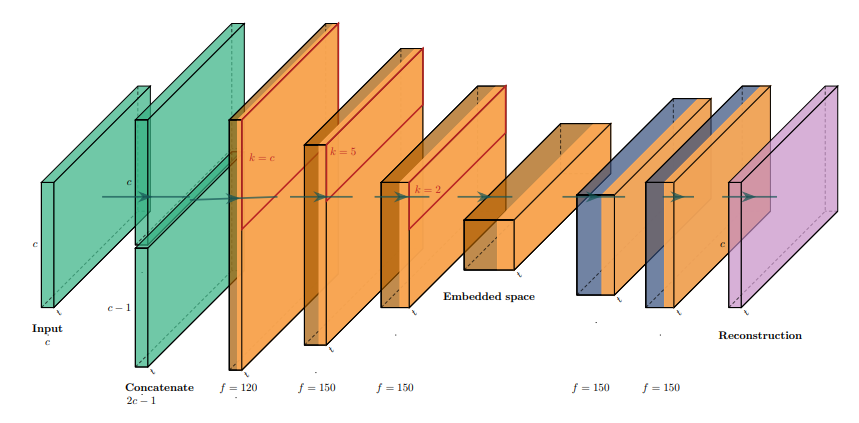
\includegraphics[width=0.8\textwidth]{Images/autoencoder_periodic_convolution.png}
    \caption{Autoencoder architecture with periodic convolutions implementation. \citep{laguarta2023detection}}
    \label{fig:autoencoder_laguarta}
\end{figure}
The autoencoder architecture is seen in Figure \ref{fig:autoencoder_laguarta}, each convolution layer is accompanied by a ReLU (Rectified Linear Unit) activation function. Despite the lowered dimensionality in the autoencoder, it is still very high. The t-SNE method can be applied for further dimensionality reduction. 
The results indicated that the autoencoder reconstruction error was highest in instances of the \verb|Scattered_Light| class. 
Safe auxiliary channel \acrshort{fd} analysis can be beneficial for noise detection and classification. Extending the proposed technique to other interferometers and investigating possible safe auxiliary channels - data strain glitch correlations is recommended.

\subsection{Glitch identification from Environmental data}
A study by \citep{colgan2020efficient} extracts useful statistical information from auxiliary channels in the vicinity of a glitch (in a 2.5 second timewindow), the acquired data is then used in a logistic regressor classifier. To limit the amount of weights, elastic net regularization \citep{zou2005regularization} is applied for penalisation. 
The results vary around 80 \% accuracy, but it does not predict the glitch class, only if it is a possible glitch or not. 

\subsection{LIGO's fourth observing run}
The initial evaluation of the fourth observing run (04) highlighted constraints in the architecture of the Gravity Spy machine learning model. Its simplicity led to challenges in generalization and the incapacity to effectively process inputs from multiple time windows \citep{wu2024advancing}. The drawbacks of the Gravity Spy classifier, as indicated in \citep{jarov2023new, alvarez2023gspynettree}, primarily include the significance of the location within the images. A line positioned at the top or bottom of the images is crucial as it represents various glitches at different frequencies. This characteristic poses difficulties for the traditional \acrshort{cnn} architecture in capturing distinctive features in glitch classes. Additionally, the shallow network structure necessitates substantial resizing of input dimensions, leading to a loss of information. Finally, the classifier struggles with an issue of confidence overfitting. In their study, researchers \citep{wu2024advancing} suggest a new architecture and compare three fusion strategies.
\newpage
\subsection{Incremental learning}
\label{ref:sub_incremental}
\subsubsection{Introduction}
In \acrshort{il} or also called \acrshort{cl}, we feed the data progressively to the model and thus acquire new knowledge over time (just as humans do). It is especially useful and efficient in learning from sequential, non-stationary data, such as wave signals. 
\citep{van2022three} illustrates the three scenarios of \acrshort{il} in terms of input $X$, context $C$ and within-context output space $Y$. 

\begin{table}[H]
\begin{tabularx}{0.9\textwidth}{l | X | l}
    \textbf{Scenario} & \textbf{Description} & \textbf{Mapping} \\
     Task-incremental learning & sequential learning of distinct task solutions. & $f:X\times C \mapsto Y$  \\
     Domain-incremental learning & Problem-solving in different contexts.&$f:X\mapsto Y$\\
     Class-incremental learning & Incrementally observed class discrimination & $f:X\mapsto C\times Y$

\end{tabularx}
     \caption{Incremental learning scenarios at computational level from \citep{van2022three}}
     \label{tab:incr_learning}
\end{table}

\begin{figure}[H]
    \centering
    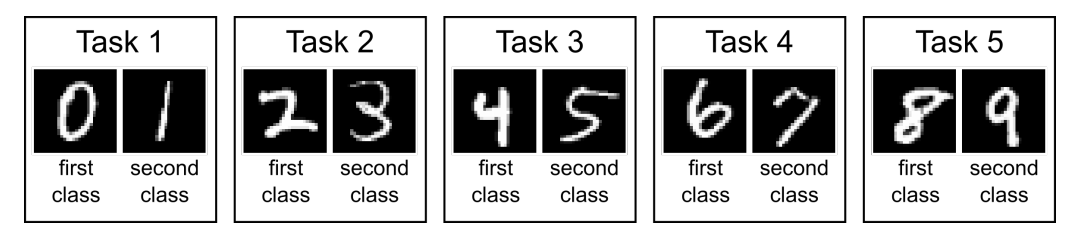
\includegraphics[width=0.9\textwidth]{Images/tasks_example_mnist.png}
    \caption{Schematic view of an MNIST task protocol, from \citep{van2019three}}
    \label{fig:mnistTaskProtocol}
\end{figure}


Looking at figure \ref{fig:mnistTaskProtocol} we can split MNIST according to the three scenarios as follows: 
\begin{table}[H]
\begin{tabularx}{0.9\textwidth}{l | X }
    \textbf{Scenario} & \textbf{Description} \\
     Task-incremental learning & With task given, is it the first or second class? (e.g. 0 or 1)  \\
     Domain-incremental learning & With task unknown, is it a first or second class? (e.g. in [0,2,4,6,8] or in [1,3,5,7,9]?\\
     Class-incremental learning & With task unknown, which digit is it? (e.g. choice from 0 to 9)

\end{tabularx}
     \caption{Split MNIST according to three scenarios from \citep{van2019three}}
     \label{tab:mnist_tasks}
\end{table}
The first scenario, Task-incremental learning (or Task-IL), involves an algorithm learning a set of distinct tasks sequentially, where the task identity is explicitly provided or clearly distinguishable. Models can be trained with task-specific components, or even use separate networks for each task. This approach avoids the problem of catastrophic forgetting (adapting to a different distribution usually leads to a significant decrease in the ability to capture the original ones \citep{wang2023comprehensive}) altogether \citep{ruvolo2013ella, masse2018alleviating}. But the main challenge is to effectively share the learnt representations while optimising the performance-complexity trade-off \citep{lopez2017gradient, vogelstein2020representation}. 

The second scenario, Domain-incremental learning (or Domain-IL) encompasses an algorithm's ability to learn a sequence of tasks characterised by the same underlying problem structure (same classes) but varying contextual and in input distributions \citep{ke2021classic, mirza2022efficient}. Unlike the first scenario, the algorithm is not explicitly informed about the task at the test time. However, the output space remains consistent between tasks, indicating generalisability to unseen tasks \citep{aljundi2017expert}. 
As explained in \citep{mirza2022efficient} domain-incremental learning can be used to learn the same set of objects (classes) over a variety of weather conditions (domains), while having access to the task-ID (current weather), this is illustrated in Figure \ref{fig:domain-incremental-weather}. 

\begin{figure}[H]
    \centering
    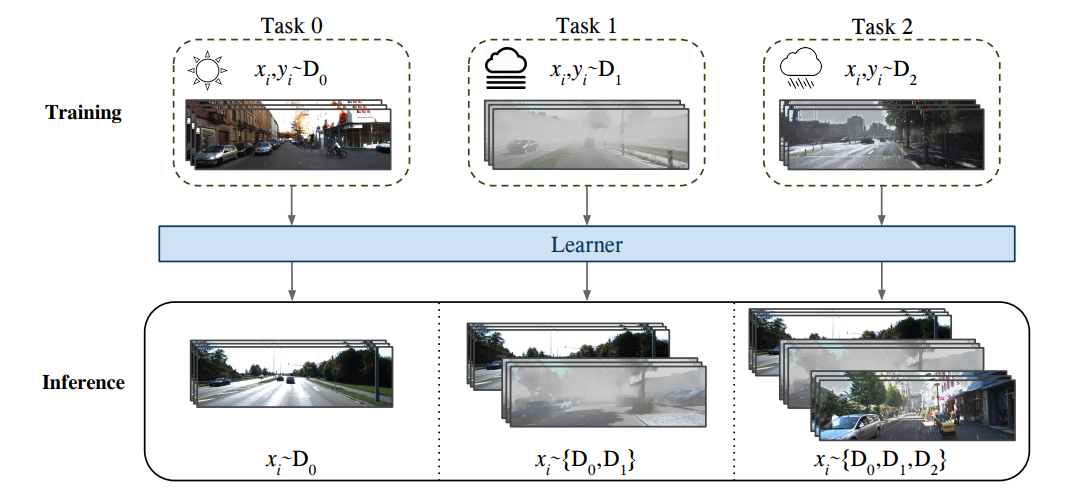
\includegraphics[width=0.9\textwidth]{Images/domain_incremental_weather.png}
    \caption{Domain-incremental learning setting. Different tasks correspond to different weather conditions which are learned in the training phase. During inference, the performance of the current task is evaluated along with all the previously seen tasks. \citep{mirza2022efficient}}
    \label{fig:domain-incremental-weather}
\end{figure}


The final scenario, Class-incremental learning (Class-IL), involves an algorithm learning to distinguish between a sequentially expanding set of classes or objects. The common setup involves encountering a sequence of classification tasks, where each task introduces new classes, and the algorithm must learn to classify samples across all accumulated classes \citep{von2019continual, van2020brain}. Task identification is crucial here as it determines the set of potential classes for a given sample. In essence, the algorithm must master both within-episode classification (distinguishing between classes in the same episode) and between-episode classification (identifying which episode a sample belongs to). This scenario presents a significant challenge to overcome catastrophic forgetting (see \ref{ref:subsub_catastrophic}), as the algorithm must not only maintain previously learned classes, but also adapt to new ones without degrading performance on previously learned classes \citep{belouadah2021comprehensive, masana2022class}. 

As illustrated in Figure \ref{fig:task-vs-class-il}, Task-IL involves having a task identifier available during inference, eliminating the need for methods to differentiate between classes from various tasks. On the other hand, in Class-IL, the learner does not have access to the task identifier during inference, requiring it to differentiate between all classes across tasks. 

\begin{figure}[H]
    \centering
    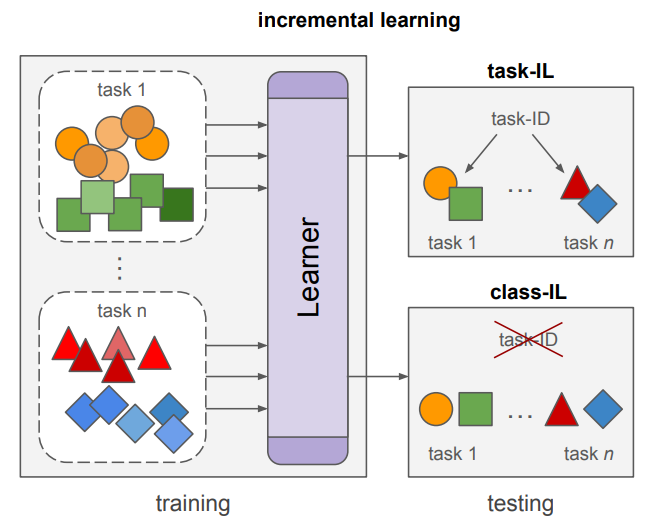
\includegraphics[width=0.6\textwidth]{Images/task_vs_class_il.png}
    \caption{In incremental learning, disjoint tasks are learned sequentially. Task-IL has access to the task identifier during evaluation, while class-IL does not. \citep{masana2022class}}
    \label{fig:task-vs-class-il}
\end{figure}

Empirical comparison of some \acrshort{dl} training strategies was executed on the MNIST \citep{deng2012mnist} and CIFAR-100 \citep{cifar} datasets. A baseline network with two fully connected hidden layers with a softmax output layer was used to compare performance.\\ 
The \acrshort{xdg} and the separate network methodology \citep{masse2018alleviating} require context knowledge of the training record, so they can only be applied in Task-IL scenarios. Regularisation methods such as \acrshort{ewc} \citep{kirkpatrick2017overcoming} employ a quadratic penalty term for each previously learnt context, effectively preventing parameter changes that would significantly deviate from the values acquired during context-specific training. 
Task-IL scenarios performed equally well as opposed to the baseline method, domain-IL and especially class-IL had a considerable drop in performance. The parameter regularisation implied a significant reduction. Replay-based algorithms had the best results for all scenarios of \acrshort{il}. \citep{khare2021unsupervised} found that the use of class imbalance improves detection in class-IL approaches.\\

\section{Background}
\label{sec:Background}
\subsection{CL Concepts and formulation}
\label{subsec:cl_concepts}
We follow the framework proposed by \citep{lesort2020continual}. 
In the context of continual learning, the data can be considered as coming from a (potentially infinite) sequence $\mathbf{D}$ of distributions that are not known in advance. This sequence, denoted as $\mathbf{D} = \{ D_{1}, ..., D_{N} \}$, is defined over the random variables $X$ and $Y$, where $X$ represents the input and $Y$ represents the output. At each time step $i$, the algorithm receives a training set $Tr_{i}$ consisting of one or more observations drawn from the distribution $D_{i}$. A learning task is marked by a distinct task label $t\in \{ 1,\dots,T\}$ and its intended goal or objective function $h^{*}$.

An algorithm with the signature $A^{CL}$, also known as a \acrlong{cl} algorithm, is defined as follows: \begin{equation} \label{eq:CL_algo} A_{i}^{CL} : \langle h_{i-1}, Tr_{i}, M_{i-1}, t_{i} \rangle \leftarrow \langle h_{i}, M_{i} \rangle \quad , \forall D_{i} \in \mathbf{D} \end{equation} In this equation, $h_i$ represents the current model or hypothesis that is continuously learned at time $i$. $M_{i}$ is an external memory buffer that stores previous training examples. $t_{i}$ is a task label associated with the training examples, and $Tr_{i}$ represents the training set of examples.

\acrshort{cl} methodologies are specific settings where the sequence of $N$ task labels follows a defined pattern over time. There are three commonly observed situations: \begin{itemize} \item Single Incremental Task (SIT): the task remains the same throughout. \item Multi Task (MT): each new task is different from the previous one. \item Multi Incremental Task (MIT): the model may encounter a combination of new and old tasks, which can be presented in an interleaved manner. \end{itemize} Task incremental scenarios assume that task labels are available for each sample. However, it is challenging to obtain explicit task labels for each sample in real-world applications \citep{cossu2021continual}.

The classification of \acrshort{cl} strategies can be categorised into three distinguishable groups: regularisation strategies, architectural strategies, and replay strategies \citep{parisi2019continual}. 

Regularisation strategies aim to achieve a balance between plasticity and stability by incorporating regularisation terms into the loss function. Example regularisation strategies are \acrshort{ewc} (see \ref{sec:ewc}), \acrshort{si} (see \ref{sec:si}) and \acrshort{lwf} (see \ref{sec:lwf}). 

The goal of a \acrshort{cl} algorithm is to learn how to accurately classify, at any specific training stage, examples from all of the observed tasks up until the current one $t\in \{ 1, \dots, t_{c} \}$:
\[
    \underset{\theta}{\mathrm{argmin}} \; \sum^{t_{c}}_{t=1} \mathbf{L}_{t}
\]
where
\[
    \mathbf{L}_{t} = \EX \left( L \left( y, f_{\theta} (x) \right) \right)
\]
and $\EX$ is the expectation over data sampled from a distribution $\mathbf{D}_t$. \\

\subsection{Catastrophic forgetting}
\label{ref:subsub_catastrophic}
While \acrshort{ml} models often achieve or even exceed human-level performance on specific tasks, they lack the ability to adapt dynamically to new data. Unlike humans, who learn concepts sequentially and reinforce their understanding by observing new examples, neural networks suffer from a phenomenon known as catastrophic forgetting \citep{french1999catastrophic}. This means that they need to be retrained from scratch every time new data becomes available. 
The dilemma (or trade-off) of Stability-Plasticity pertains to the capacity to incorporate new information while preserving past knowledge during the process of recoding \citep{grossberg2012studies}. Neural networks often tend to be skewed towards too much plasticity (integrating new knowledge) \citep{de2021continual}. Forgetting is, not only related to machines, it is part of the very nature of learning (e.g. forgetting biased information). The decay of forgetting can be described by a power law. When a person is taught a specific concept, if there is no repetition or emotional significance attached to it, the information is quickly forgotten but not entirely erased. Over time, forgetting follows a declining pattern \citep{pashler2009predicting}.


\subsection{CL training methods}
In the subsequent section, we will outline a few of the frequently employed training techniques. Most of the training strategies follow the guidelines of General Continual Learning (GCL) as proposed by \citep{farquhar2018towards}. 
\begin{itemize}
    \item Do not rely on task boundaries.
    \item No oracle with task identifiers during testing.
    \item A bounded constant memory throughout training.
\end{itemize}

\subsubsection{Elastic Weight Consolidation}
\label{sec:ewc}
The study by \citep{kirkpatrick2017overcoming} and \citep{de2021continual} explains \acrshort{ewc} is a regularization method designed to address the issue of catastrophic forgetting in neural networks. It achieves this by constraining the learning process. The main concept behind \acrshort{ewc} involves incorporating a quadratic penalty term into the standard loss function. This penalty term takes into account the difference between the current weight values and the optimal weights that were obtained during the previous task learning phase. By doing so, \acrshort{ewc} minimises interference between tasks and ensures a balance between learning new tasks and retaining knowledge from previous tasks.
\begin{figure}[h]
\centering
    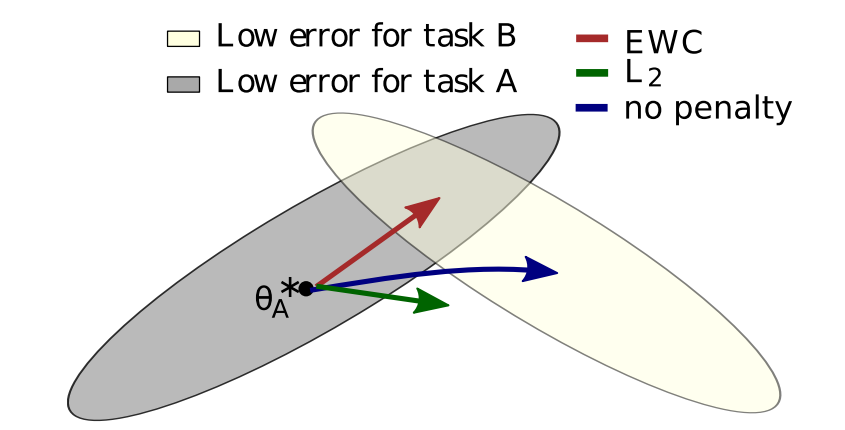
\includegraphics[width=0.7\textwidth]{Images//ewc.png}
    \caption{EWC guarantees task A is remembered while training on B. \citep{kirkpatrick2017overcoming}}
    \label{fig:ewc}
\end{figure}
The concept of Elastic Weight Consolidation (EWC) allows for the retention of knowledge from task A while training on task B. The training process is represented in a conceptual parameter space (Figure \ref{fig:ewc}), where regions of parameters resulting in good performance on task A are depicted in grey, and those for task B are depicted in cream color. Once task A is learned, the parameters are located at $\theta_{A}^{*}$ (see Figure \ref{fig:ewc}). However, when considering the gradient steps of task B (blue arrow in Figure \ref{fig:ewc}), the loss of task B is minimized but at the expense of compromising the knowledge acquired from task A, this is equivalent to "no penalty": \[ \theta^* = \underset{\theta}{\mathrm{argmin}} \, \mathbf{L}_B(\theta) \] To prevent forgetting the learned knowledge from task A, a distance minimization technique is applied between $\theta$ and $\theta^{*}_{A}$ ($L_{2}$ in Figure \ref{fig:ewc}): \[ \theta^{*} = \underset{\theta}{\mathrm{argmin}} \, \mathbf{L_B(\theta)} + \frac{1}{2} \alpha ( \theta - \theta_{A}^{*} )^{2} \] Here, $\alpha$ is a scalar that determines the relative importance of the old task compared to the new one. 
The constraint of $L_{2}$ is highly restrictive and has the capacity to hinder the learning process of task B. In the realm of deep learning, it is common practice to excessively parameterize models. Some parameters may be less beneficial while others hold greater significance.

\acrshort{ewc} discovers a solution for task B without significantly impairing task A's performance (red arrow in Figure \ref{fig:ewc}) by explicitly calculating the importance of each weight for task A. This importance value, also called the Fisher Information matrix\footnote{The Fisher Information Matrix provides a curvature approximation of the loss function \citep{ly2017tutorial}}, quantifies the weight's contribution to the performance on previously learned tasks. Weights with higher importance values have a greater impact on the performance of the previous tasks. The learning process is formulated as follows: 
\[
\theta^{*} = \underset{\theta}{\mathrm{argmin}} \; \mathbf{L_B}(\theta) + \frac{1}{2} \lambda I_{\theta_{A}^{*},i}(\theta_{i} - \theta_{A,i}^{*})^{2}
\]
In the above equation, $L_{\theta_{A}^{*},i}$ represents the diagonal elements of the Fischer information matrix, and $\lambda$ is the hyperparameter that determines the strength of the regularization penalty.
The implementation operates by computing the Fisher information matrix $I_{i}$ for each batch $B_{i}$. This is achieved by conducting a forward and backward propagation of the patterns. Subsequently, the implementation stores the obtained $I$ and the optimal weights $\theta$.


\subsubsection{Synaptic Intelligence}
\label{sec:si}
According to \citep{zenke2017continual} and \citep{maltoni2019continuous}, the introduction of \acrshort{si} as a modification to \acrshort{ewc} involved performing the computationally expensive Fisher matrix computations online during \acrshort{sgd} throughout the learning process. The implementation of this approach involves calculating the weight importance matrix $I_{i}$ for each batch of data samples $B_{i}$ using the information already available during \acrshort{sgd}. The weight importance matrix $I$ and the optimal weights $\theta$ are then stored.


\subsubsection{Learning without Forgetting}
\label{sec:lwf}
The aim of the \acrshort{lwf} approach is to manage the process of forgetting by enforcing output stability (Maltoni et al., 2019). It follows a similar approach to parameter regularization methods like EWC (see Section \ref{sec:ewc}) and SI (see Section \ref{sec:si}), where a regularization term is added to the classification loss function $\mathbf{L}$. Although originally designed for classification tasks, it has also been successfully utilized in 
object detection \citep{de2021continual}.


\subsubsection{FROMP}
\label{sec:fromp}
The \acrshort{fromp} training strategy is a novel approach in \acrshort{cl} addressing the catastrophic forgetting problem. It regularises the network outputs at a few memorable past examples that are crucial to avoid forgetting. By using a Gaussian process formulation of deep networks, the approach enables training in weight-space while identifying both the memorable past and a functional prior. It involves a slight modification of the Adam optimizer and a minor increase in computational cost. \citep{pan2020continual}. A schematic representation of \acrshort{fromp} is depicted in figure \ref{fig:fromp}. 
\begin{figure}
    \centering
    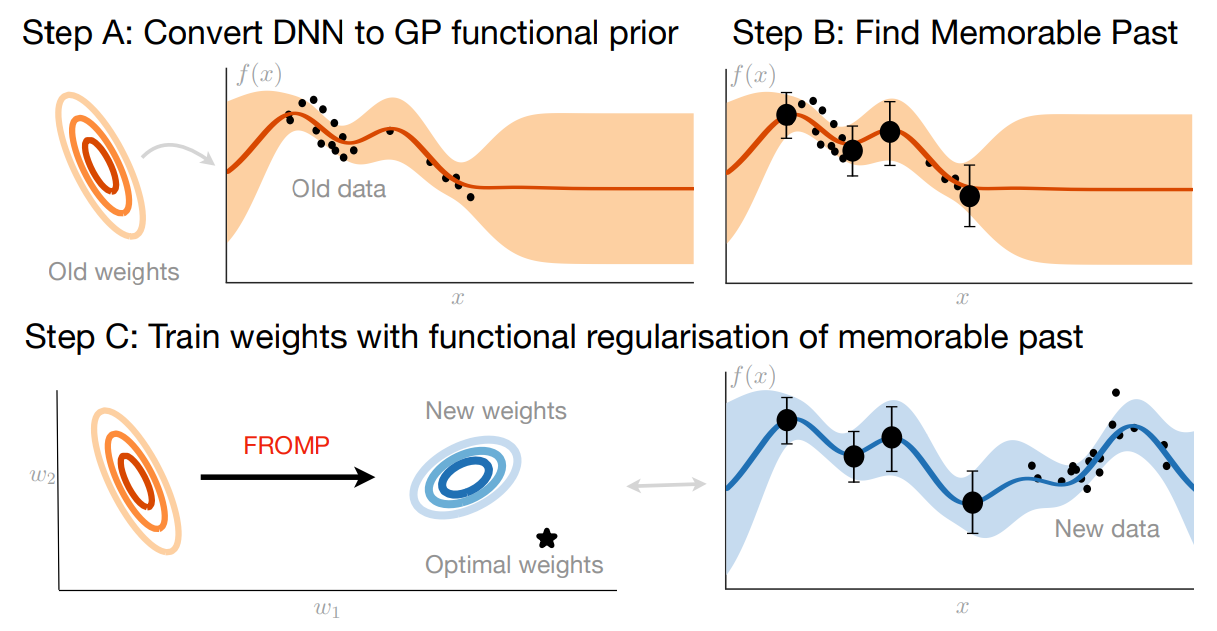
\includegraphics[width=0.8\textwidth]{Images//fromp.png}
    \caption{The FROMP method consists of three main steps where they first convert a DNN (Deep Neural Network) to a GP (Gaussian-Process), find memorable examples, and train weights with functional regularisation of those examples. \citep{pan2020continual}}
    \label{fig:fromp}
\end{figure}

\subsubsection{GEM}
\label{sec:gem}
The \acrlong{cl} (\acrshort{cl}) strategy, proposed by \citep{lopez2017gradient}, is a model that overcomes the limitations imposed by Empirical Risk Minimization \citep{vapnik1991principles} on other supervised learning techniques. To bridge this gap, the \acrlong{gem} (\acrshort{gem}) model incorporates an episodic memory $M_t$ that selectively stores a subset of observed examples from a specific task $t$. The memory capacity is limited to a total of $M$ locations, with each task having $m=\frac{M}{T}$ memories. The examples stored in $M$ are utilized to determine predictor functions $f_{\theta}$ by minimising the corresponding loss function
\[
\mathbf{L}(f_{\theta}, M_{k}) = \frac{1}{|M_{k}|} \sum_{(x_i, k, y_i) \in M_{k}} \mathbf{L}(f_{\theta}(x_i , k), y_i)
\]
Overfitting to the stored examples in $M_{k}$ is a common issue when minimizing the loss at the current example along with the above loss function. To address this problem, they solve the following optimization problem:
\[ 
\underset{\theta}{\mathrm{argmin }} \; \mathbf{L}(f_{\theta}(x,t),y) \text{ subject to } \mathbf{L}(f_{\theta}, M_{k}) \leq \mathbf{L}(f_{\theta}^{t-1}, m_k), \forall k<t 
\]
Here, $f^{t-1}_{\theta}$ represents the previous predictor state at the end of learning task $t-1$. The detailed solution can be found in the original paper by \citep{lopez2017gradient}.


\subsubsection{A-GEM}
\label{sec:a-gem}
\citep{chaudhry2018efficient} proposes a more efficient version of \acrshort{gem} where it tries to ensure that at every training step the average episodic memory loss over the previous tasks does not increase. Formally the objective of \acrshort{agem} is
\[ 
\underset{\theta}{\mathrm{argmin }} \; \mathbf{L}(f_{\theta} D_{t}) \text{ such that } \mathbf{L}(f_{\theta}, M) \leq \mathbf{L}(f_{\theta}^{t-1}, M), \text{ where } M = \underset{k<t}{\bigcup} M_{k} 
\]
The detailed solution and update rule can be found in the original paper by \citep{chaudhry2018efficient}.

\subsubsection{iCaRL}
As described in \citep{rebuffi2017icarl} iCaRL (Incremental Classifier and Representation Learning) allows learning in a class incremental way as depicted in figure \ref{fig:icarl}. It learns strong classifiers and a data representation simultaneously. In iCaRL, the model learns to recognize new classes while retaining its ability to recognize old ones. This is achieved by storing examples of each class, which are selected based on their closeness to the mean feature of that class. 
The model is then trained on both the new data and these examples. This approach ensures that the model does not forget the old classes when learning new ones. 

\begin{wrapfigure}{l}{0.40\textwidth}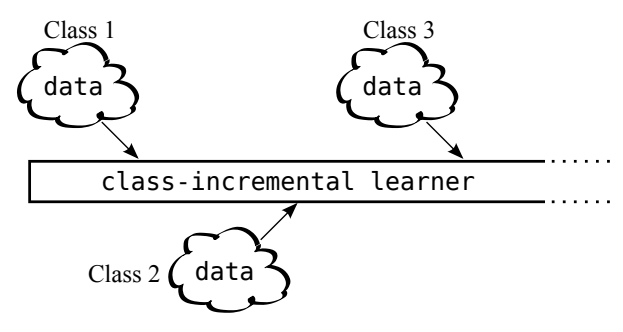
\includegraphics[width=0.45\textwidth]{Images//class_incremental_learning.png}
    \caption{Class-incremental learning. \citep{rebuffi2017icarl}}
    \label{fig:icarl}
\end{wrapfigure}


iCaRL utilizes a \acrshort{cnn} as its underlying mechanism. The \acrshort{cnn} functions as a feature extractor that can be trained, denoted as $\phi: X \rightarrow \mathbf{R}^{d}$, followed by a single classification layer containing sigmoid output nodes equal to the number of classes encountered up to that point. All feature vectors undergo $L^{2}$ normalization. The classification approach employed by iCaRL is based on a nearest-mean-of-exemplars strategy.\\
In order to predict a label, $y^{*}$, for a new input, $x$, the system calculates a prototype vector for each class seen so far, represented as $\mu_{1}, ..., \mu_{t}$, where $\mu_{y}$ represents the average feature vector of all examples belonging to class $y$. It also computes the feature vector of the image that should be classified and assigns the class label with the most similar prototype: 
\[
y^{*} = \underset{y=1,...,t}{\mathrm{argmin }} \| \phi(x) - \mu_{y} \|
\]

\subsubsection{SCR}
\label{sec:SCR}
\begin{wrapfigure}{r}{0.40\textwidth}
    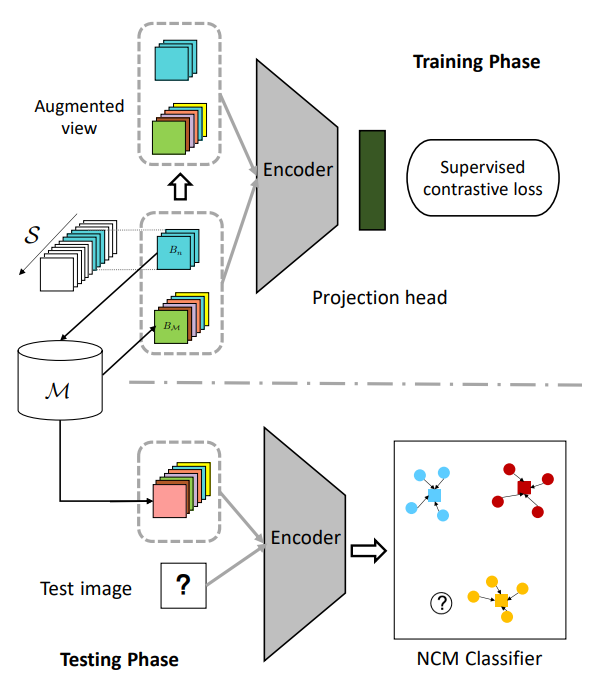
\includegraphics[width=0.40\textwidth]{Images/scr_architecture.png}
    \caption{A schematic view of SCR. \citep{mai2021supervised}}
    \label{fig:scr_architecture}
\end{wrapfigure}

\acrfull{scr} is a technique introduced by \citep{mai2021supervised} to address some challenges common in \acrshort{cl}. 
Because the softmax classifier is not the best choice for CL approaches, it aims to leverage the \acrfull{ncm} classifier instead to effectively mitigate catastrophic forgetting (or also called task-recency bias).\\
The \acrshort{scr} process (see Figure \ref{fig:scr_architecture}) involves the creation of an input batch during training by combining a minibatch $B_{n}$ from the datastream with another minibatch $B_{M}$ from the memory buffer $M_{i}$.\\ 
These input batches, along with their augmented views, are encoded by a shared encoder  and projection head. Followed by an evaluation using supervised contrastive loss. In the testing phase, the projection head is removed. Supervised Contrastive Loss is an alternative loss function to cross entropy that can leverage label information more effectively. \citep{khosla2020supervised}.

\subsubsection{DER and DER++}
\acrfull{der} is proposed by \citep{buzzega2020dark} as an improvement on Experience Replay (ER) while maintaining a simple formulation. It relies on dark knowledge for distilling past experiences, sampled over the training trajectory. \\
Formally, given a \acrshort{cl} classification split in $T$ tasks

It is problematic that the data from earlier tasks $\mathbf{D}_{t}$ for $t \in \{ 1, \dots, t_{c} - 1 \}$ is unavailable. To preserve the knowledge acquired previously, the subsequent objective function, which mirrors the teacher-student method, is minimized:

\[
\mathbf{L}_{t_{c}} + \alpha \sum_{t=1}^{t_{c}-1} \EX \left[ D_{KL} \left( f_{\theta_{t}^{*}}(x) \parallel f_{\theta}(x) \right) \right]
\]
where $\theta_{t}^{*}$ is the optimal set of parameters at the end of task $t$, $\alpha$ is a hyperparameter balancing the trade-off between the terms. 
$D_{KL}$ stands for the Kullback-Leibler divergence, a measure of how one probability distribution diverges from a second, expected probability distribution. It is commonly used to quantify how much knowledge from previous tasks is retained or lost when learning new tasks \citep{goodfellow2016deep}.\\
The above objective function requires having access to $\mathbf{D}_{t}$ for earlier tasks. To address this issue, a replay buffer $M_{t}$ is utilized to store previous experiences related to task $t$. Instead of preserving the actual labels $y$, the network logits (pre-activation outputs) $z \doteq h_{\theta_{t}}(x)$ are maintained. 
\[
\mathbf{L}_{t_{c}} + \alpha \sum_{t=1}^{t_{c}-1} \EX \left[ D_{KL} \left( \sigma(z) \parallel f_{\theta}(x) \right) \right]
\]
where $\sigma$ is the softmax function and $(x,z)$ are drawn from the replay buffer $M_{t}$. \\
\acrshort{der} uses reservoir sampling as defined by \citep{vitter1985random} to select $|M|$ random samples from the input stream, this way guaranteeing the same probability of being stored in the buffer without knowing the length in advance. This way the previous equation (with $\EX$ drawn from $M$) becomes:
\[
\mathbf{L}_{t_{c}} + \alpha \EX \left[ D_{KL} \left( \sigma(z) \parallel f_{\theta}(x) \right) \right]
\]

Given some basic assumptions, as mentioned in \citep{hinton2015distilling}, maximizing the KL divergence corresponds to minimizing the Euclidean distance among the logits. Consequently, the target function for \acrshort{der} is defined as
\[
\mathbf{L}_{t_{c}} + \alpha \EX \left[ \| z - h_{\theta}(x) \|^{2}_{2} \right]
\]

with $\EX$ being approximated by gradient computation on batches sampled from the replay buffer \citep{buzzega2020dark, boschini2022class}. \\
\acrshort{der++} adjusts the objective function by adding an additional balancing term $\beta$ on alternative 'buffer' data points

\[
\mathbf{L}_{t_{c}} + \alpha \EX \left[ \| z_{1} - h_{\theta}(x_{1}) \|^{2}_{2} \right] + \beta \EX \left[ \mathbf{L} \left( y_{2}, f_{\theta}(x_{2}) \right) \right]
\]

\acrshort{der++} collapses to \acrshort{der} when the coefficient $\beta=0$. \\
Experiment results, as described in \citep{buzzega2020dark} conclude that \acrshort{der} converges to more flat minima and to more calibrated networks. 

\subsection{CL metrics}
\label{sec:il_metrics}
Evaluation of learning tasks is a major part of research. As \citep{qu2021recent} indicates, not only the performance on new tasks, but also the amount of forgotten wisdom must be considered. We follow the notation used in \citep{diaz2018don, lopez2017gradient, chaudhry2018riemannian} to define the most popular metrics. \\
We denote $a_{q,p}$ as the accuracy on the separate test set of the task $p$ after \acrshort{il} of $q$ previous tasks, where $p\leq q$.

\subsubsection{Average accuracy ($A_{q}$)}
The metric $A_{q}$, as explained in \citep{wang2023comprehensive}, is utilized to assess the effectiveness of the \acrshort{il} model. It is calculated by averaging the accuracies obtained after learning a total of $q$ tasks. 
\begin{equation}
\label{metric:A_q}
    A_{q} = \frac{1}{q} \sum_{p=1}^{q} a_{q,p}
\end{equation}
This method is employed to assess the capacity to retain information from previous tasks while acquiring new knowledge.

\subsubsection{Average forgetting ($F_{q}$)}
The metric $F_{q}$, which is described in \citep{qu2021recent}, quantifies the amount of knowledge that is forgotten during the first $q-1$ tasks. It is calculated using the formula \begin{equation}
\label{metric:F_q}
    F_{q} = \frac{1}{q-1} \sum_{p=1}^{q-1} f_{p}^{q} 
\end{equation} 
where $f_{p}^{q}$ represents the knowledge forgotten for task $p$. This is determined by subtracting the remaining knowledge after learning $q$ tasks from the maximum knowledge obtained during the \acrshort{il} process. In eq. \ref{metric:F_q}, $f_{p}^{q}$ is calculated as follows: 
\begin{equation}
\label{metric:f_p_q}
  f_{p}^{q} = \max_{o \in \{ 1, ..., q-1\}} a_{o,p} - a_{q,p} , \forall p < q.
\end{equation}

\subsubsection{Intransigence ($I_{q}$)}
The metric called Intransigence (or learning plasticity) quantifies the extent to which \acrshort{cl} hinders a model from learning a new task in comparison to traditional batch learning. It is calculated as follows: 
\begin{equation}
\label{metric:I_q}
    I_{q} = a^{*}_{q} - q_{q,q}
\end{equation} 
In eq. \ref{metric:I_q}, $a^{*}_{q}$ represents the accuracy achieved on the test set of the $q^{\text{th}}$ task when batch learning is employed for all $q$ tasks \citep{chaudhry2018riemannian}.

\subsubsection{Backward transfer ($BWT_{q}$)}
The concept of backward transfer, as described in \citep{lopez2017gradient}, is how much the learning process on task $q$ affects the performance of previously learned tasks. This can be quantified using the following equation: \begin{equation}
\label{metric:BWT_q}
BWT_{q} = \frac{1}{q-1} \sum_{p=1}^{q-1} (a_{q,p} - a_{p,p})
\end{equation}

\subsubsection{Forward transfer ($FWT_{q}$)}
Forward transfer refers to the degree to which the continuous learning of the $q^{\text{th}}$ task has the potential to influence the performance of future tasks. In \citep{lopez2017gradient}, the accuracy on the test set of the $p^{\text{th}}$ task at random initialization is represented as $b_{p}$. The forward transfer metric, denoted as $FWT_{q}$, is defined as follows: \begin{equation} FWT_{q} = \frac{1}{q-1} \sum_{p=2}^{q} (a_{p-1,p} - b_{p}) \end{equation}
\citep{wang2023comprehensive}

\subsection{Multimodal Fusion}
\acrshort{dl} models increasingly interact through multiple modalities, such as vision, text, touch, ... Each modality provides a unique perspective on the environment. Multimodal Fusion is the technique for integrating information from different modalities, in case of glitch detection this could be the spectrogram image and the calculated fractal dimensions. By effectively fusing information, models can achieve superior performance in various tasks. \\
\citep{ngiam2011multimodal, gao2020survey, zhang2021exploring}
Fusing different modalities is one of the challenges in multimodal learning. There are two approaches (see Figure \ref{fig:earlyVsLate} commonly used, 'Early Fusion' and 'Late Fusion'. Depending on the location of the fuse operation. 

\begin{figure}[ht]
    \centering
    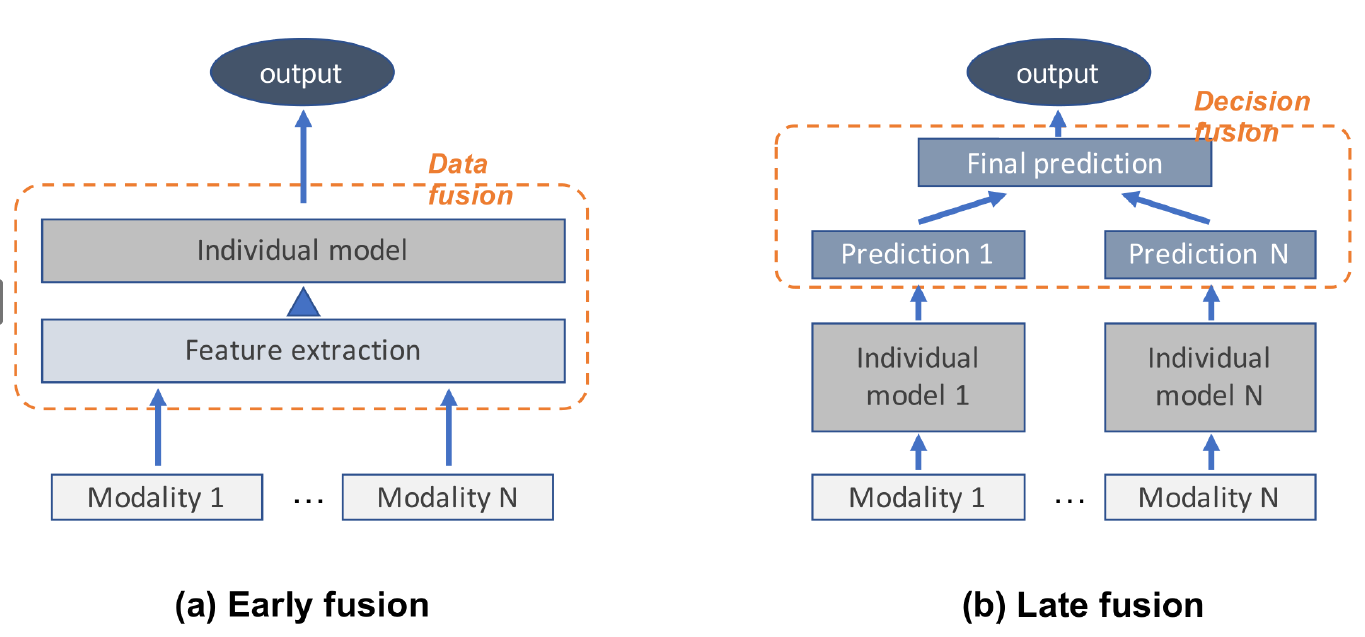
\includegraphics[width=0.9\textwidth]{Grad Assignment/Images/EarlyVsLate_fusion.png}
    \caption{Early vs Late Fusion \citep{kim2021multimodal} }
    \label{fig:earlyVsLate}
\end{figure}

To define Early and Late Fusion, let $M$ represent the total number of modalities. Each modality input is represented as a vector $\mathbf{v}_{m}$. We assume a K-class classification scenario where $y$ represents the labels. The prediction probability of the $k$-th class from the $m$-th modality is denoted by $p_{m}^{k}$, and the final prediction probability of the $k$-th class by the model is denoted by $p^{k}$. \citep{liu2018learn}\\

\newpage
With Early Fusion, features from different modalities are combined at the input level. If for instance we have a text and image, early fusion merges the raw text and image features before feeding them into the model. This assumes that all modalities have compatible representations.\\

In Early Fusion, a unified model $h$ is trained to capture the relationships and interactions among low-level features. The resulting prediction is given by 
\[
p = h([\mathbf{v}_{1}, ..., \mathbf{v}_{m}])
\]
Early Fusion has a simple pipeline because only one model is needed for training.\\

With Late Fusion, each modality is processed independently and their features are combined at a later stage. This allows each modality to learn its own representations and then combines them.\\
Late Fusion combines unimodal decision values through a fusion mechanism $F$ (such as averaging, voting, etc.). Given that $h_{i}$ is applied to modality $i$, the final prediction is
\[
p = F\left( h_{1}(\mathbf{v}_{1}), ..., h_{m}(\mathbf{v}_{m})\right)
\]
This approach permits the utilization of various models, providing greater adaptability.
\\

Usually, specialized networks are employed for various modalities to produce their respective representations, which are then combined or aggregated. Subsequently, a prediction is made based on the aggregated representation, typically using another neural network to capture the interactions between the different modalities. Summation (or averaging) and concatenation are two frequently used aggregation techniques. 
\[
\mathbf{u} = \left[ f_{1}(\mathbf{v}_{1}), ..., f_{m}(\mathbf{v}_{m}) \right]
\]
where $f_{m}$ is a domain specific neural network. 
Given the combined vector output $\mathbf{u}$, another network $g$ computes the final output
\[
p = g(\mathbf{u})
\]

\citep{liu2018learn, gadzicki2020early, wang2022comprehensive}




\subsection{Python packages}
A recent toolbox called \verb|PyCIL| \citep{zhou2023class, zhou2023pycil} implements several state-of-the-art \acrshort{il} algorithms. The package \verb|Avalanche| \citep{lomonaco2021avalanche} provides a library for benchmarking, training, prototyping, training and evaluation of \acrshort{cl} algorithms. Continuum \citep{douillard2021continuum} is a library that provides data loading functionalities for \acrshort{cl}. 

\subsubsection{Avalanche}
\label{sec:avalanche}
The Avalanche package came into existence with a clear goal in mind, \textit{"Pushing Continual Learning to the next level, providing a shared and collaborative library for fast prototyping, training and reproducible evaluation of continual learning algorithms."} \citep{avalancheContinualAIFiveMinutes}

Avalanche is structured based on a series of core design principles: 1) minimizing code length for rapid prototyping and error minimization, 2) ensuring reproducibility, 3) promoting modularity and reusability, 4) enhancing code efficiency, scalability, and portability and 5) prioritizing usability.


\begin{figure}[H]
    \centering
    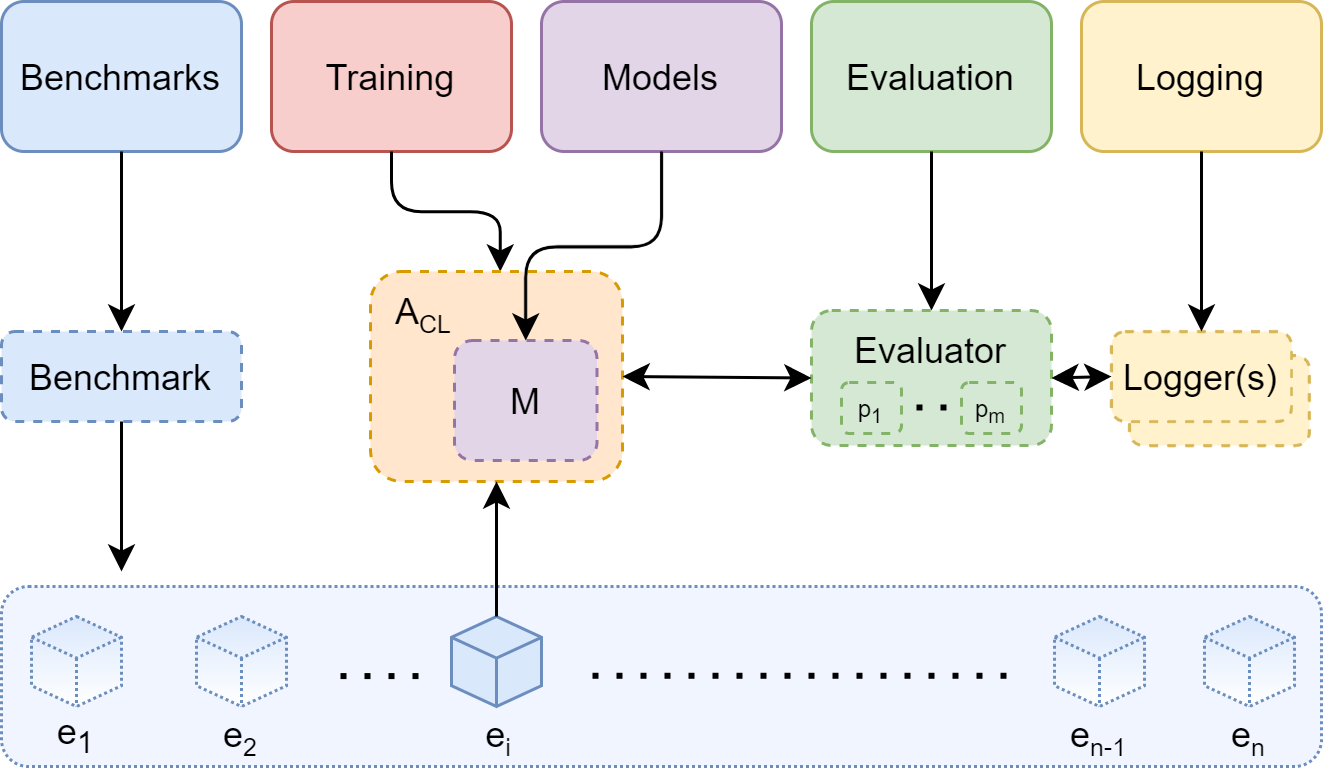
\includegraphics{Images//avalanche.png}
    \caption{The main Avalanche modules and how they interact with each other. \citep{avalancheContinualAIFiveMinutes} }
    \label{fig:avalanche}
\end{figure}
Avalanche is organized in five main modules denoted in figure \ref{fig:avalanche}. 

1) \textbf{Benchmarks}: This component preserves a consistent application programming interface (API) for managing data, primarily by producing a sequence of data from multiple datasets. It contains the primary \acrshort{cl} performance metrics (similar to the approach taken in \verb|torchvision| ).

2) \textbf{Training}: This module offers a comprehensive range of tools related to model training. It encompasses straightforward and effective methods for incorporating new continual learning strategies, along with a collection of pre-implemented \acrshort{cl} baselines and cutting-edge algorithms that can be utilized for comparison purposes.

3) \textbf{Evaluation}: This module offers a comprehensive set of tools and measurements that can help evaluate a \acrshort{cl} algorithm in relation to the various factors that we consider crucial for a system that learns continuously.

4) \textbf{Models}: In this module, you will discover various model structures and pre-trained models suitable for your ongoing learning experiment (similar to what has been done in \verb|torchvision.models|).

5) \textbf{Logging}: It contains sophisticated logging and visualization functionalities, such as built-in support for \verb|stdout|, file, and \verb|Tensorboard| (Effortlessly monitor your experiment metrics in real-time using just one line of code on a comprehensive interactive dashboard). 

\citep{lomonaco2021avalanche, carta2023avalanche}

\subsection{Saliency Mapping}
The Image-Specific Class Saliency Visualisation is a method described in \citep{simonyan2013deep} for understanding a \acrshort{cnn} decision-making process by visualizing the spatial support of a particular class within a given image. The goal is to rank the pixels of an input image based on their influence on the score function, which indicates the likelihood of the presence of a specific class.
Given an image $I_{0}$, a class label $c$ and a \acrshort{cnn} classifying score function $S_{c}(I_{0})$, we would like to rank the pixels of $I$ based on their influence on the score $S_{c}(I)$. 
The linear score model, where the score $S_{c}$ is determined by the dot product between the weight vector $w_{c}$ and the image $I$, and adding a bias term $b_{c}$. 
\[
S_{c}(I) = w_{c}^{T} I + b_{c}
\]
In this model, the importance of individual pixels in the image for the class $c$ is directly proportional to the magnitude of the corresponding elements in the weight vector $w_{c}$. However, the class score function is non-linear, therfore the linear model cannot be applied. 
The purpose of the Class Saliency Visualisation is to address this non-linearity in \acrshort{cnn}'s. Given an image $I_{0}$, the class score $S_{c}(I)$ can be approximated with a first-order Taylor expansion: 
\[
S_{c}(I) \approx w^{T} I + b
\]
where $w$ is the partial derivative of $S_{c}$ w.r.t. the image $I$ at the point $I_{0}$: 
\[
w = \left. \frac{\partial S_{c}}{\partial I} \right|_{I_{0}}
\]
The above approach aims to infer the importance of pixels in an image for a specific class despite the non-linear nature of the classifier. This visualization method helps in understanding how the model makes its predictions by highlighting which parts of the image contribute most significantly to the classification of a particular class. 

The class saliency map $M\in \mathbf{R}^{m\times n}$ for an image $I_{0}$ (of size $m\times n$) and a class $c$ requires a single back-propagation pass through the classification \acrshort{cnn}. The elements of the derivative $w$ are then rearranged. 

In case of a grey-scale image, the mapping is computed as $M_{ij} = \left| w_{h(i,j)} \right|$ where $h(i,j)$ is the corresponding pixel-index of $w$ in row $i$ and column $j$. 

In case the image is an RGB-image, the color channel $c$ must be taken into account. The authors \citep{simonyan2013deep} opt for the maximum value of $w$ over the different color channels: $M_{ij} = \max_{c} \left| w_{h(i,j,c)}\right|$

\begin{figure}[!hb]
    \centering
    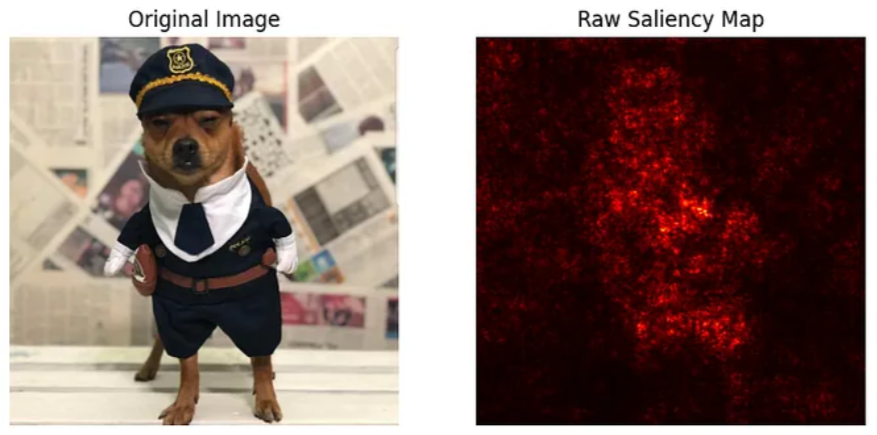
\includegraphics[width=0.5\textwidth]{Grad Assignment/Images/saliency_example.png}
    \caption{Example saliency map and original image. Taken from \citep{newginsam2024}}
    \label{fig:saliency_example}
\end{figure}






\chapter{Research methodology}
\section{Research}
\label{sec-Research}
\subsection{Research questions}
The upcoming research will investigate the following questions:  

\begin{mdframed}[backgroundcolor=lightgray!20]
\par RQ1: Do classes learned from a continual learning approach align with existing gravity spy classes?\\
RQ2: How effective are continual learning approaches when incorporating auxiliary channel data for detecting and classifying glitch morphologies?\\
RQ3: What if strain data (spectrograms) are combined with auxiliary channel data in a multimodal approach? Does this learn a robust classification?
\end{mdframed}

\subsection{Research method}
\label{subsec-researchmethod}
\subsubsection{RQ1}
In order to evaluate the alignment between classes acquired from a \acrlong{cl} approach and existing gravity spy classes, we proceed with the following steps:
\begin{itemize}
    \item Data preprocessing is required for the utilization of a \acrshort{cl} approach, involving the selection of either the O3a or O3b dataset that includes labeled data with various glitch categories. This dataset will be segmented into sequential chunks to represent a continuous data stream.
    \item Model selection and Training: A proper \acrshort{cl} algorithm will be chosen, taking into account aspects such as memory usage and its ability to reduce catastrophic forgetting. The model will be trained gradually on the segmented data, mimicking a continual learning scenario.
    \item In order to assess the alignment, we will compare the classes acquired from the \acrshort{cl} model with the existing gravity spy classes. This assessment could include traditional measures like accuracy and confusion matrix, as well as the specific metrics for \acrshort{cl} outlined in Section \ref{sec:il_metrics}. 
\end{itemize}
\subsubsection{RQ2}
In order to assess how well auxiliary channel-based strategies work for detecting and categorizing glitch shapes, we will utilize the following approach:
\begin{itemize}
    \item The dataset preparation will be done by gathering glitch-affected and clean signal samples. Useful information needs to be extracted from a selection of auxiliary channels in a limited time window around glitch transients. The approach of \citep{colgan2020efficient} will be used. 
    \item A Convolutional-based architecture will be used, together with the same selection of \acrshort{cl} algorithms, used in RQ1. 
    \item Evaluating the model's performance is done by using metrics like precision, recall and F1-score. Additionally visualization techniques can be employed to understand the relative feature importance of selected auxiliary channels for glitch classification. 
\end{itemize}
\subsubsection{RQ3}
To investigate the main challenges in implementing \acrfull{cl} and explore mitigation strategies, we will take a two-pronged approach: 
\begin{itemize}
    \item The dataset used in RQ2, together with the spectrograms provided by Melissa Lopez, will be used. 
    \item A multimodal fusion architecture will be used to incorporate auxiliary channel data alongside the spectrogram dataset. The model will be trained to learn robust glitch detection and classification. 
    \item Evaluating the model's performance is done by using metrics like precision, recall and F1-score. Additional visualization techniques such as \acrshort{tsne}, \acrshort{umap} and Saliency mapping will be used. 
\end{itemize}

\chapter{Models and Results}
\section{Technical aspects}
The code repository containing all notebooks, models and results can be found via \newline \url{https://github.com/brianbaert/MscThesis.git} 


All the experiments were done on a single GPU server with the following specifications:
\begin{table}[H]
\centering
\begin{tabular}{|l|l|}
\hline
\textbf{Processors} & 4x Intel(R) Xeon(R) 3-2286G CPU @ 4.00GHz \\
\hline
\textbf{Operating System} & Microsoft Windows Server 2022 Datacenter \\
\hline
\textbf{GPU} & NVIDIA RTX A4500 (20GB) \\
\hline
\textbf{RAM} & 32 GB \\
\hline
\end{tabular}
\label{tbl:specifications}
\caption{Server specifications}
\end{table}

\section{Data description}
\label{sec-DataDesc}
\subsection{Gravity Spy dataset}
The dataset includes 23 different types of glitches represented by time-frequency spectrograms. These glitches have been detected using the Omicron trigger pipeline \citep{robinet2020omicron}, which applies specific criteria such as identifying real-time events with a \acrshort{snr} above 7.5 and a peak frequency ranging from $10 Hz$ to $2048 Hz$. Subsequently, the strain data is transformed into time-frequency spectrograms using the Q-transform process \citep{chatterji2004multiresolution}, these spectrograms are also known as Omega scans.
Gravity Spy produces four spectrograms for every detected glitch, utilizing different time windows: 0.5s, 1.0s, 2.0s, and 4.0s. An illustration of a "Koi Fish" anomaly is depicted in figure \ref{fig:koifish}, while an instance of a "Whistle" anomaly is displayed in figure \ref{fig:whistle}.
\begin{figure}[H]
    \centering
    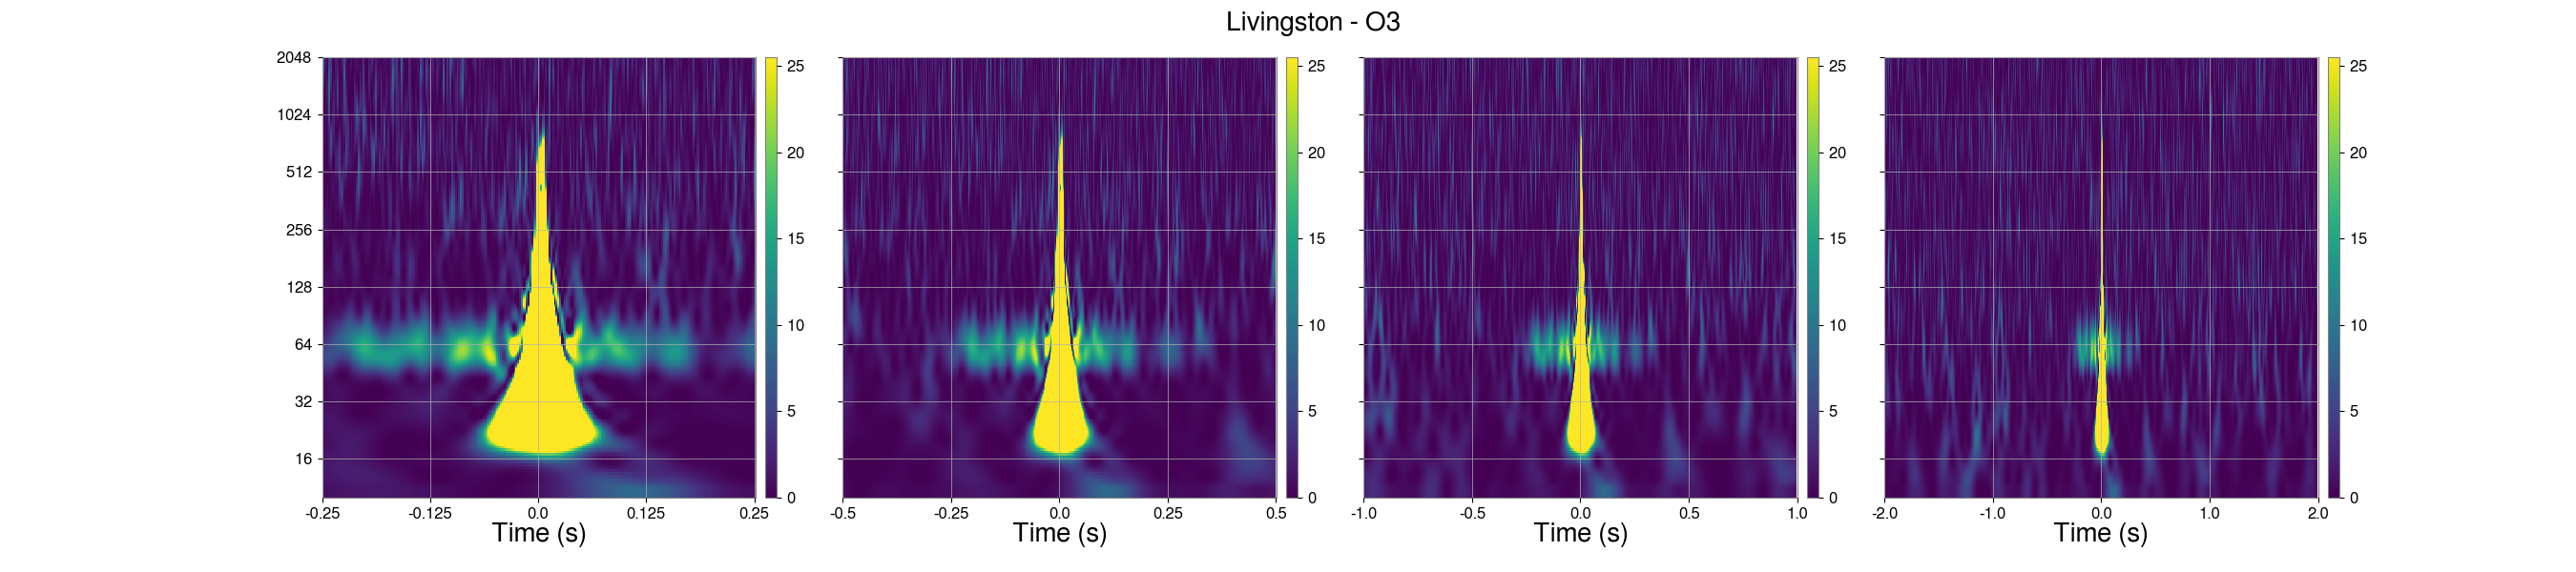
\includegraphics[width=0.9\textwidth]{Images/koi_fish_1250427024.302.png}
    \caption{Spectrogram example of a Koi Fish glitch with four time windows (0.5s, 1.0s, 2.0s an 4.0s}
    \label{fig:koifish}
\end{figure}
\begin{figure}[H]
    \centering
    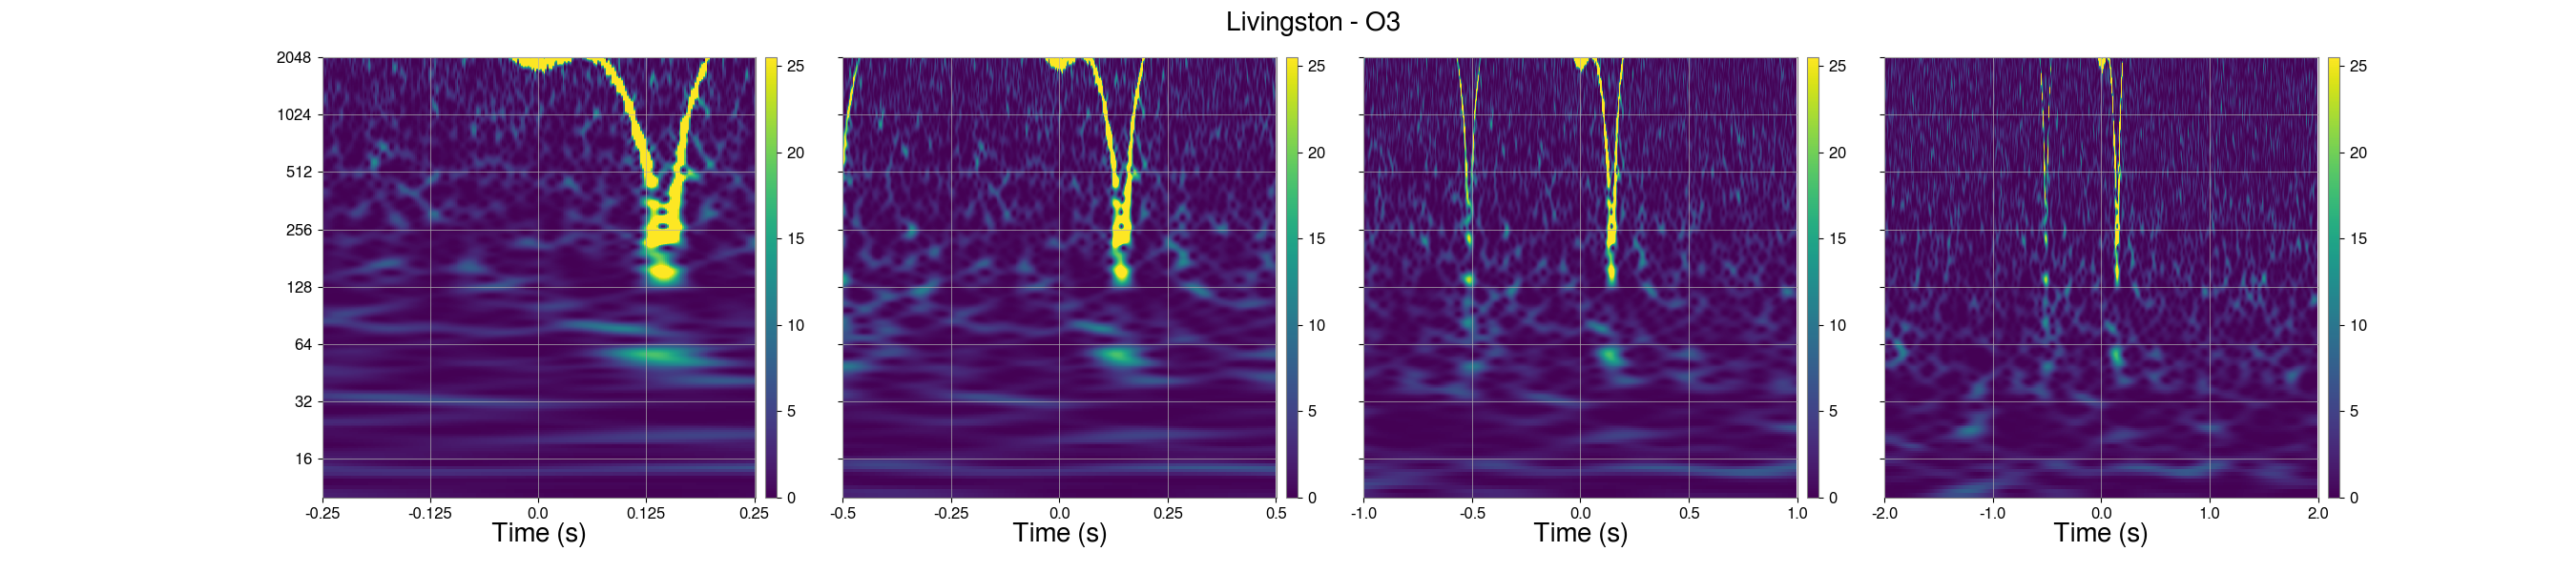
\includegraphics[width=0.9\textwidth]{Images/whistle_1239025005.518.png}
    \caption{Spectrogram example of a Whistle glitch with four time windows (0.5s, 1.0s, 2.0s an 4.0s}
    \label{fig:whistle}
\end{figure}
The class names were established collaboratively by LIGO and citizen scientists. However, there may be a noisy-label problem in the ground truth, as some misclassifications of glitches occurred by both the classifier and volunteers. Hence, it is essential to focus on glitches with a confidence score exceeding 0.9. The dataset shows an imbalance, with O3a having mostly Fast scattering and Tomte glitches, whereas O3b contains mainly Scattered light or Fast scattering glitches. Preliminary results (obtained from LigoDV-Web\footnote{https://ldvw.ligo.caltech.edu/ldvw/gspySearch}) of O4a are mainly Low Frequency burst (45,8\%) and Low Frequency lines (33,1\%) . 

\subsection{O3 Auxiliary Channel data}
As described on the GWOSC\footnote{https://gwosc.org/O3/auxiliary/} website, the O3 auxiliary channel dataset includes channels (more than 200 000 per detector) that were used to create data quality flags, subtract instrumental noise from the strain data and measure the amount of correlated noise between the \acrshort{gw} detectors. 
Data quality flags play a crucial role in the O3 auxiliary channel data, serving to eliminate time periods where data integrity may be compromised by instrument-related or environmental interference. At times, an auxiliary channel may capture extraneous noise sources such as scattered light or power frequency variations, enabling \acrshort{ligo} to enhance the accuracy of strain data by removing such noise components. Conversely, an auxiliary channel can also serve as an indicator of detector glitches, signaling instances of malfunction to analysts for data reliability assessment. Nonetheless, this approach may be flawed if auxiliary channels inadvertently detect disturbances in the gravitational wave channel, leading to the simultaneous appearance of an astrophysical signal in both channels. Channels that detect heightened power levels from the gravitational wave channel are labeled as "unsafe" for vetoing purposes, while those unaffected by this interference are deemed "safe." Vetoing of gravitational wave candidates relies solely on data from "safe" channels. 

Each channel is identified by a name following the format \verb|[IFO]:[SYSTEM]-[NAME]| , where \verb|[IFO]|  denotes the instrument (L1, H1, ...), \verb|[SYSTEM]|  specifies the subsystem (PSL, IMC, TCS, PEM, ...), and \verb|[NAME]|  provides a description of the channel. The dataset available on the GWOSC website comprises 40 channels from the collective \acrshort{ligo} detectors (Hanford, Livingston) that were utilized in the O3 analysis. The dataset has a total size of 13 TB, the full channel list can be found via the \acrshort{ligo} git repository\footnote{https://git.ligo.org/gwosc/}
\citep{GravitySpy20Wiki}

\section{Model}
\subsection{Model design and parameter choices for RQ1}
The \verb|MultiViewColorNet_resnet18| architecture is a PyTorch model extending the \newline \verb|nn.Module| class. It is designed for a multi-class classification task. 
\begin{figure}[H]
    \centering
    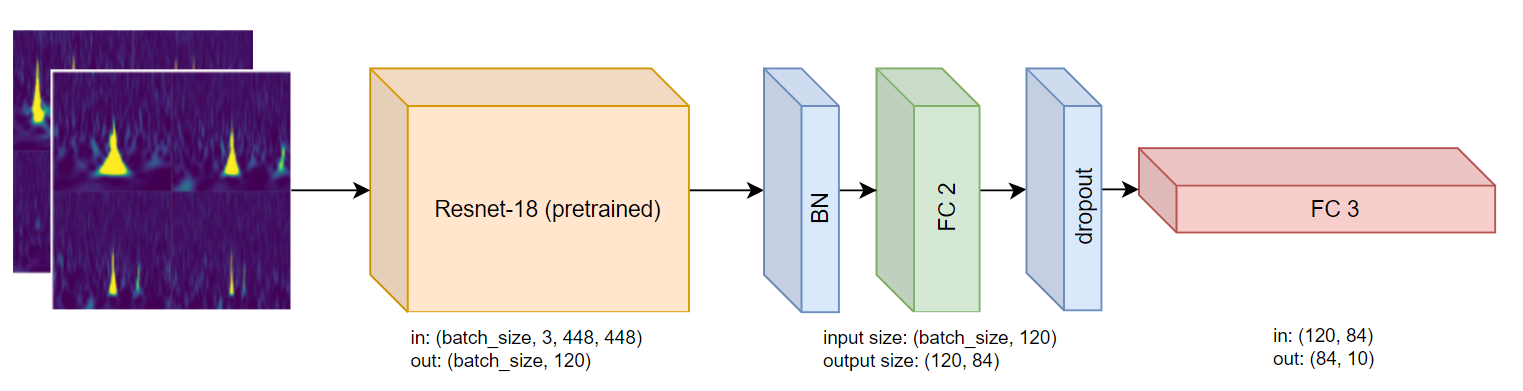
\includegraphics[width=1.0\textwidth]{Images/SlimResnet18_Multiview_CL.png}
    \caption{MultiviewColorNet\_SlimResnet18}
    \label{fig:slimresnet18_multiview}
\end{figure}
The full PyTorch implementation can be found in Appendix \ref{appendix1}, in short the implementation consists of:
\begin{itemize}
    \item A pre-trained ResNet-18 model is loaded into \verb|self.resnet|. The weights are set to 'DEFAULT' (pre-trained on ImageNet). 
    \item The kernel size of the first convolutional layer in the ResNet model is modified to (7,7), this is necessary for coping with the 448 by 448 RGB fused image. 
    \item All parameters in the ResNet model are unfrozen, allowing them to be updated during training. 
    \item The last layer of the ResNet model, a fully connected layer, is replaced with a new linear layer that has 120 output features. 
    \item Two additional fully connected layers (\verb|self.fc2| and \verb|self.fc3|) are added, with the final layer outputting a number of features equal to \verb|num_classes|.
    \item A dropout layer (\verb|self.dropout|) with a dropout probability of 0.3 is added to help prevent overfitting (according to \citep{park2017analysis} 0.3 is a good value for more complex CNN's like ResNet). 
    \item A batch normalization layer (\verb|self.bn|) is added to normalize the activations of the neurons in the network. 
\end{itemize}

The train dataset contains a balanced random selection of spectrograms from 10 glitch classes ('Blip', 'Blip\_Low\_Frequency', 'Extremely\_Loud', 'Fast\_Scattering', 'Koi\_Fish', \\
'Low\_Frequency\_Burst', 'Low\_Frequency\_Lines', 'Scattered\_Light', 'Tomte', 'Whistle')
(each datapoint consists of a 0.5, 1.0, 2.0 and 4.0 second view of the glitch). 

The spectrograms containing glitches are fused via a custom PyTorch DataLoader extending the ImageFolder class. It concatenates the views into a single image of size 448 by 448 (see Figure \ref{fig:fused_image_tomte} for an example), allowing a model to learn from all views simultaneously. This is particularly useful because different views of a glitch can provide different insights. The final image and its label are returned. 

\begin{figure}[H]
    \centering
    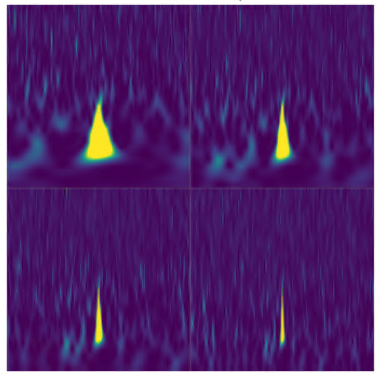
\includegraphics[width=0.5\textwidth]{Images/FusedImage_Tomte.png}
    \caption{Example of a fused image (glitch type 'Tomte').}
    \label{fig:fused_image_tomte}
\end{figure}

The Avalanche \ref{sec:avalanche} New Classes benchmark (\verb|nc_benchmark|) is used because it is specifically designed for creating benchmarks in a "New Classes" continual learning scenario, where each experience introduces new classes that were not present in the previous experiences. Here we opt for 5 experiences (2 classes per experience). \\


The optimizer for the majority of experiments is the \verb|AdamW| optimizer, a variant of the Adam optimizer including weight decay. It is often preferred over standard Adam because it handles weight decay in a more principled manner, leading to better generalization on some tasks \citep{loshchilov2019decoupled}. The learning rate is set to 0.001 and weight decay to 0.00001. These are common hyperparameter choices for AdamW. \\



The criterion used for the experiments is CrossEntropyLoss, a common choice for multi-class classification tasks. This loss function combines LogSoftmax\footnote{Applies the $\log (\text{Softmax} (x))$ function to an input Tensor. \citep{miranda2017softmax}} and NLLLoss\footnote{Negative Log Likelihood Loss \citep{miranda2017softmax}} in one single class, making it suitable for training a classification problem with more than 2 classes. 
\newpage
\subsection{Model design and parameter choices for RQ2}
The \verb|FractalDimensionConvNet| architecture is a PyTorch model extending the \newline \verb|nn.Module| class and uses a combination of convolutional layers, batch normalization, dropout and fully connected layers. It is designed for a multi-class classification task. 
\begin{figure}[H]
    \centering
    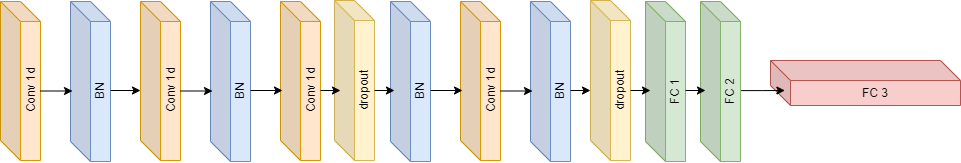
\includegraphics[width=1.0\textwidth]{Grad Assignment/Images/FD_architecture.drawio.png}
    \caption{FractalDimensionConvNet}
    \label{fig:FractalDimensionConvNet}
\end{figure}
The full PyTorch implementation can be found in Appendix \ref{appendix3}, in short the implementation consists of:
\begin{itemize}
    \item Four pairs of 1-dimensional convolutional layers (\verb|nn.Conv1d|) are used to process the fractal dimension data into a 1-dimensional format. 
    \item Fully connected Layers are added to flatten the output and output a three-class prediction. 
    \item Two dropout layers (\verb|self.dropout|) with a dropout probability of 0.1 and 0.3 are added to help prevent overfitting. 
    \item Four batch normalization layers (\verb|self.bn|) are added to normalize the activations of the neurons in the network. 
    \item The model uses the SELU (Scaled Exponential Linear Unit) activation function after each convolutional and the first fully connected layer, which can lead to self-normalizing neural networks \citep{rasamoelina2020review, kiliccarslan2021overview}. The second fully connected layer users the ReLU activation function. 
\end{itemize}

The train dataset contains a balanced (896 entries for each of the three glitch categories) selection of 2688 records where each record contains fractal dimension calculations on 50 auxiliary channels from 3 glitch classes ('Whistle', 'Tomte', 'Scattered\_Light'). Each channel has 56 fractal dimension calculations. The dataset selection is based on the study by \citep{laguarta2023detection}.

An example visualisation is show in Figure \ref{fig:FD_visualisation}
\begin{figure}[ht]
    \centering
    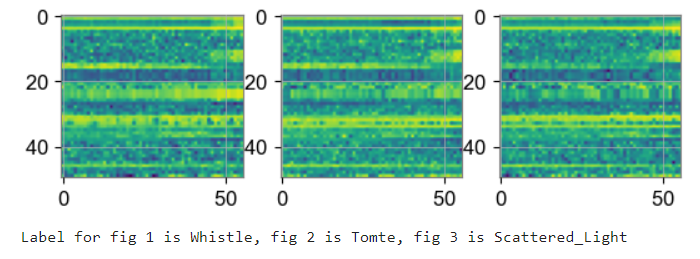
\includegraphics[width=0.5\textwidth]{Grad Assignment/Images/FD_visualisation_50channels.png}
    \caption{Example visualisations of FD matrices with 50 channels. Left = 'Whistle', Middle = 'Tomte' and right = 'Scattered\_Light'}
    \label{fig:FD_visualisation}
\end{figure}

The optimizer for the majority of experiments is the \verb|AdamW| optimizer. The learning rate is set to 0.001 and weight decay to 0.00001. Finally, the criterion used for the experiments is CrossEntropyLoss just as in \ref{subsubsec:RQ1_naive_baseline}. 
\newpage
\section{Results}
\subsection{RQ1}
\label{subsec:RQ1}
Eeach of the strategies are trained for 100 epochs on every task (of distinguishing between two glitch categories). The order in which the classes are fed is kept the same over all strategies (1 = \{Koi\_Fish; Low\_Frequency\_Burst\}, 2 = \{ Tomte; Extremely\_Loud \}, 3 = \{ Whistle; Fast\_Scattering \}, 4 = \{ Blip\_Low\_Frequency ; Scattered\_Light \} and 5 = \{ Blip; Fast\_Scattering \} )

\subsubsection{Naive CL strategy (baseline)}
\label{subsubsec:RQ1_naive_baseline}
As baseline we use the \acrshort{cl} stategy 'Naive'. This is the simplest form of \acrshort{cl}, where the model is trained on each task (in our setting we have 5 tasks (experiences) consisting of two classes per task) in sequence without any explicit mechanism to mitigate catastrophic forgetting. However, because early runs of this model suffered from extreme recency bias, the strategy is augmented with a couple of plugins to improve its performance: 
\begin{itemize}
    \item \verb|ReplayPlugin|: this plugin implements experience replay, a common technique to mitigate catastrophic forgetting. It stores a subset of the training data and interleaves training on the current task with training on the stored data. The memory size is set to twice the size of the training set, meaning it can store two complete copies of the training set. 
    \item \verb|EarlyStoppingPlugin|: This plugin implements early stopping, and thus prevents overfitting. 
\end{itemize}
During training we keep track of the weight distribution changes via violin plots. 
After the first 100 epochs training on differentiating the classes from experience 0 to 4 we get: 
\begin{center}
\begin{tabular}{cc}
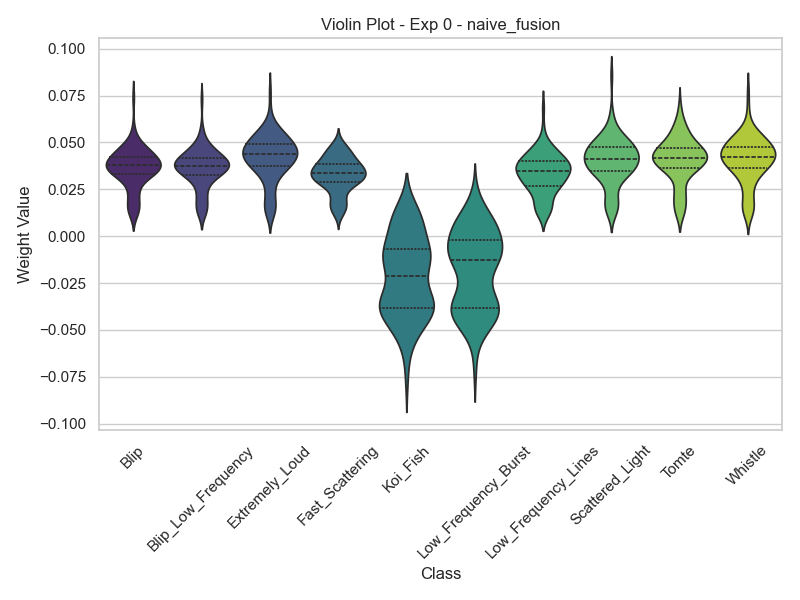
\includegraphics[width=0.4\textwidth]{Images/naive_fusion_exp_0.png} & 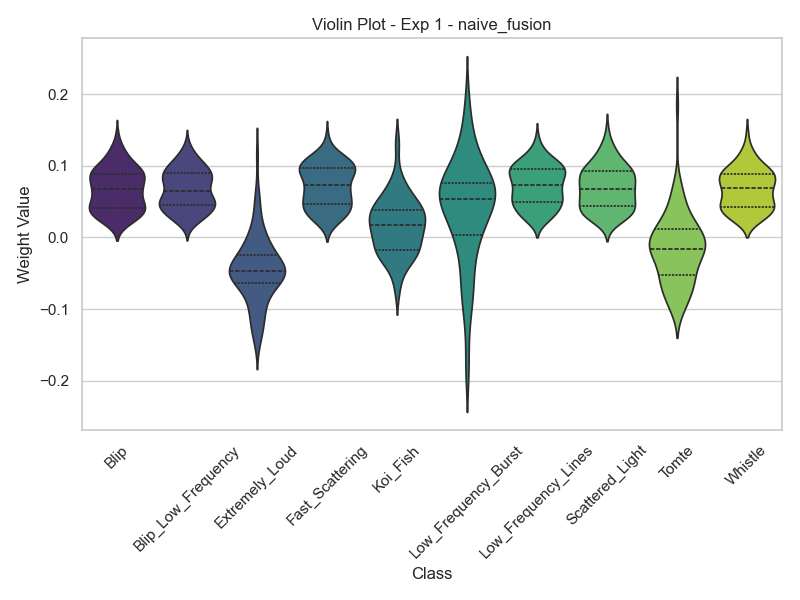
\includegraphics[width=0.4\textwidth]{Images/naive_fusion_exp_1.png} \\
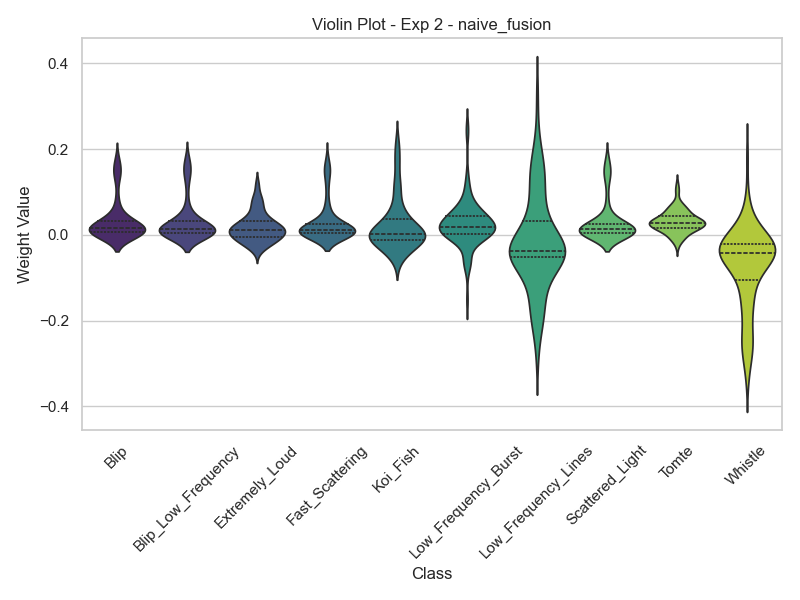
\includegraphics[width=0.4\textwidth]{Images/naive_fusion_exp_2.png} & 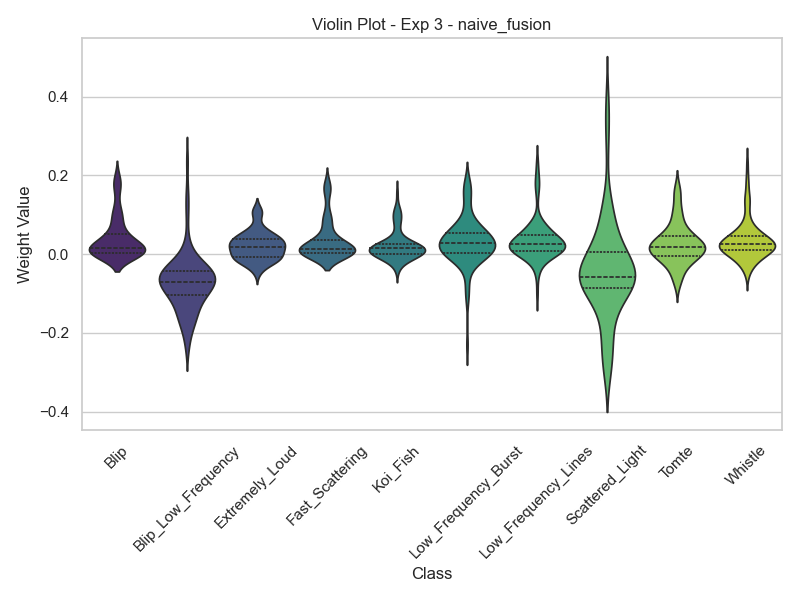
\includegraphics[width=0.4\textwidth]{Images/naive_fusion_exp_3.png}
\end{tabular}
\end{center}
\begin{center}
    \begin{tabular}{c|c}
         \multicolumn{2}{c}{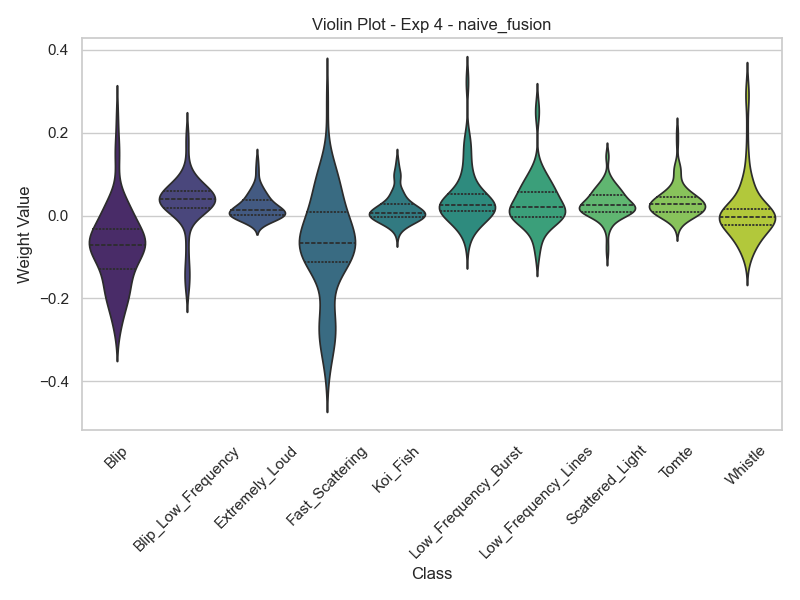
\includegraphics[width=0.4\textwidth]{Images/naive_fusion_exp_4.png}}
    \end{tabular}
\end{center}
For each experience, the weights for the Softmax classification corresponding to the classes in that experience in the fully connected layer are adjusted more than for the other classes. The median shift and distribution shape of the violin body illustrate this. 

From the Confusion Matrix as shown in Figure \ref{fig:cm_f1_naive_baseline}-(a) we find that the overall accuracy is $81.8 \%$. Some glitch classes like 'Whistle' and 'Frequency\_Lines' have perfect accuracy, whilst others like 'Blip\_Low\_Frequency' and 'Tomte' suffer from a lot of False Negatives, on the other hand 'Blip' suffers from a lot of False Positives. 

\begin{figure}[ht]
\centering
\begin{subfigure}
  \centering
  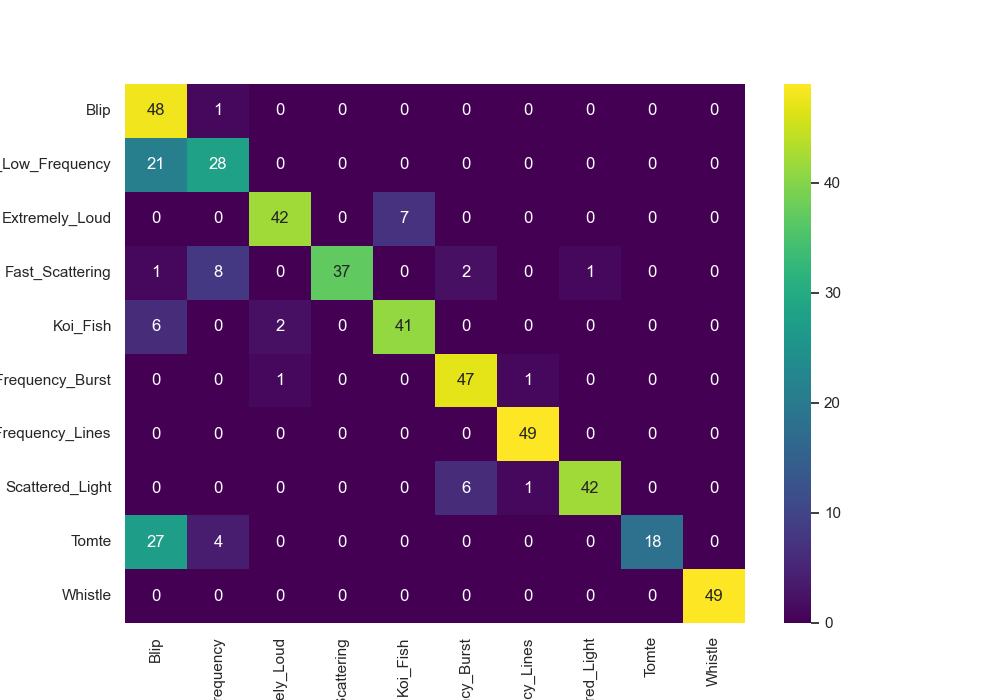
\includegraphics[width=0.49\textwidth]{Grad Assignment/Images/cm_MultiView_Naive_100epochs.png}  
  \label{fig:sub-first}
\end{subfigure}
\begin{subfigure}
  \centering
  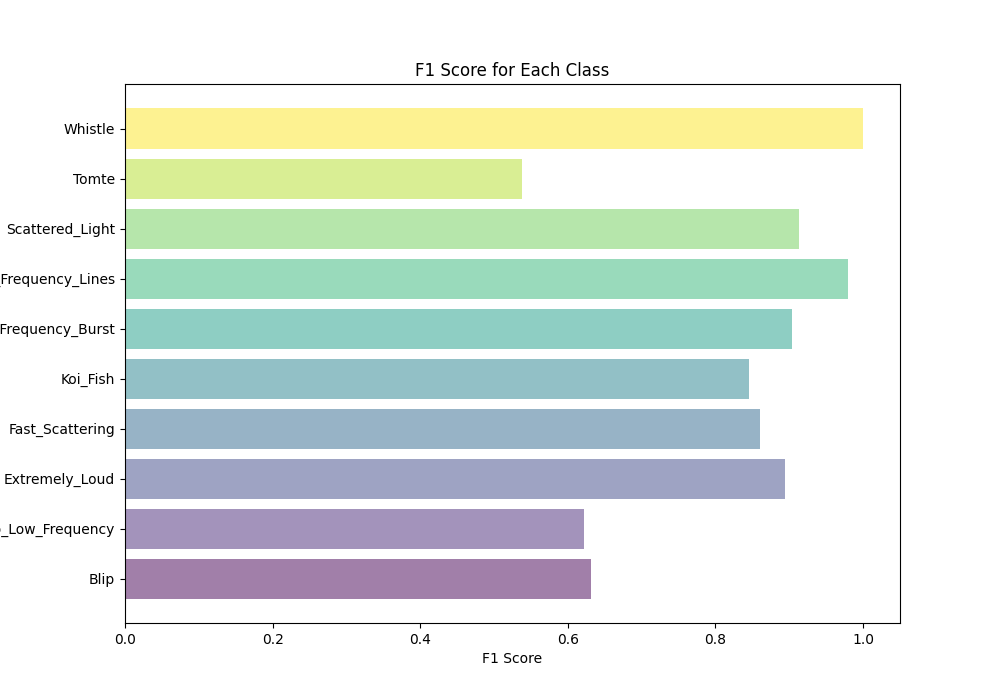
\includegraphics[width=0.49\textwidth]{Grad Assignment/Images/f1_MultiView_Naive_100epochs.png}  
  \label{fig:sub-second}
\end{subfigure}
\caption{Confusion matrix and f1 plot for Naive baseline}
\label{fig:cm_f1_naive_baseline}
\end{figure}

We investigate the \acrshort{tsne} and \acrshort{umap} representations\footnote{UMAP tends to better preserve global structure compared to t-SNE, it strikes a balance between global and local structure. \citep{mcinnes2018umap}}, 
The t-SNE visualization as shown in Figure \ref{fig:tSNE_Naive} illustrates a clustering of glitch classes in 2D space. The separation of most glitch categories like 'Whistle' and 'Scattered\_Light' is apparent. But the overlap of the Glitch categories 'Blip', 'Blip\_Low\_Frequency' and 'Tomte' could proof problematic in producing False positives for one of the three classes.
A similar interpretation can be made from Figure \ref{fig:umap_Naive}. Here 'Koi\_Fish' and 'Extremely\_Loud' as well as 'Blip', 'Blip\_Low\_Frequency' and 'Tomte' are relatively close to eachother, suggesting shared global features. 

\newpage
\begin{figure}[ht]
\centering
\begin{subfigure}
  \centering
    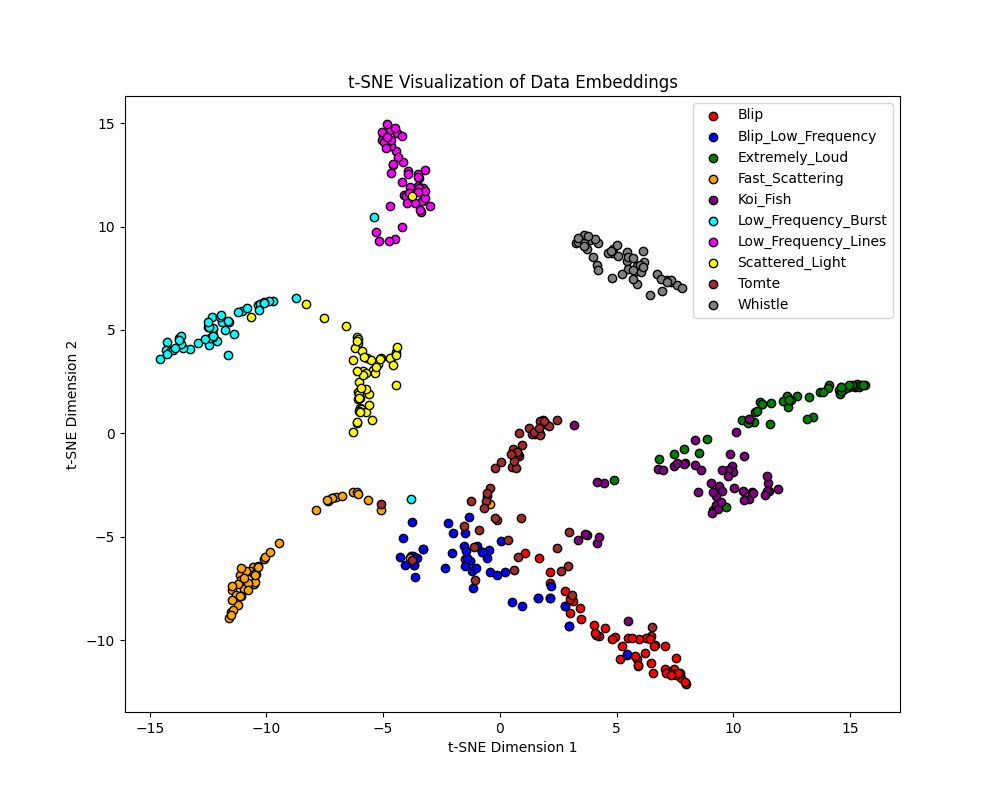
\includegraphics[width=0.6\textwidth]{Images/tSNE_MultiView_Naive_testset_100epochs.png}
    \caption{t-SNE visualization Naive strategy}
    \label{fig:tSNE_Naive}
\end{subfigure}
\begin{subfigure}
  \centering
    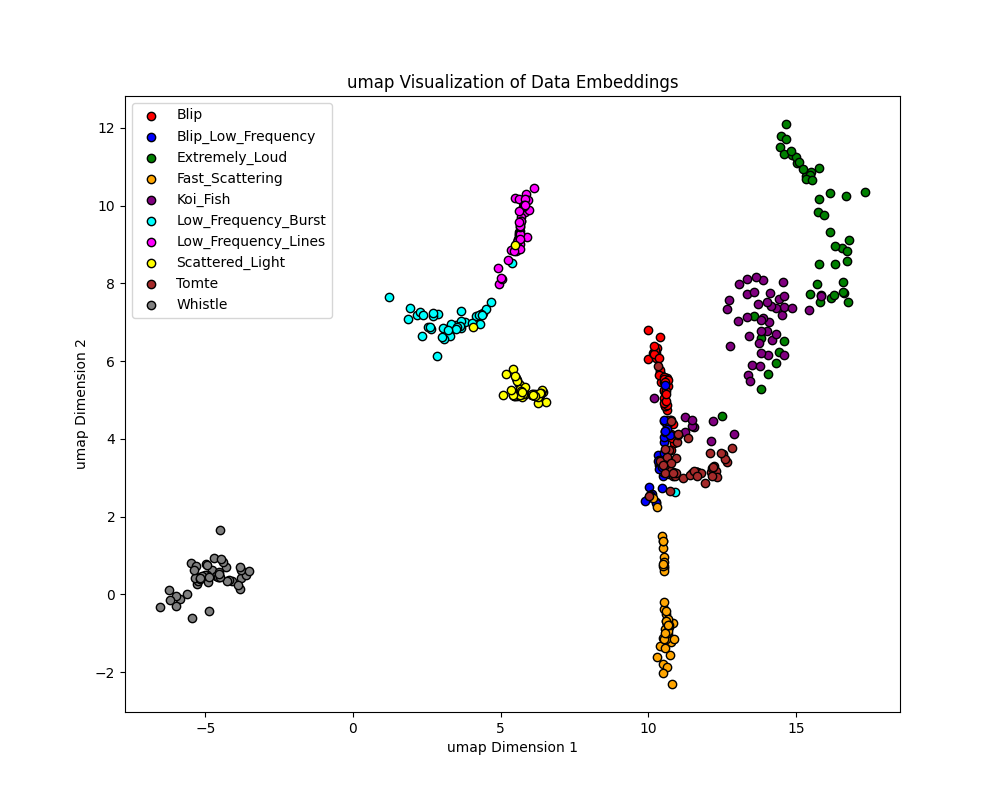
\includegraphics[width=0.6\textwidth]{Images/umap_MultiView_Naive_testset_100epochs.png}
    \caption{UMAP visualization Naive strategy}
    \label{fig:umap_Naive}
\end{subfigure}
\end{figure}

The images of the Saliency Mapping in Figure \ref{fig:saliency_naive_baseline} confirm some of the misclassifications we already concluded from the Confusion Matrix. Specifically on row 2 and row 3 we see the 'Blip\_Low\_Frequency' misclassified as a 'Blip'. It is clear that the shape of these two are very similar. 
Because 'Blip' is provided in the last experience, the recency bias favors this category. Presumably if the 'Blip\_Low\_Frequency' was used in the last experience, the results would be mirrored. 

\begin{figure}
    \centering
    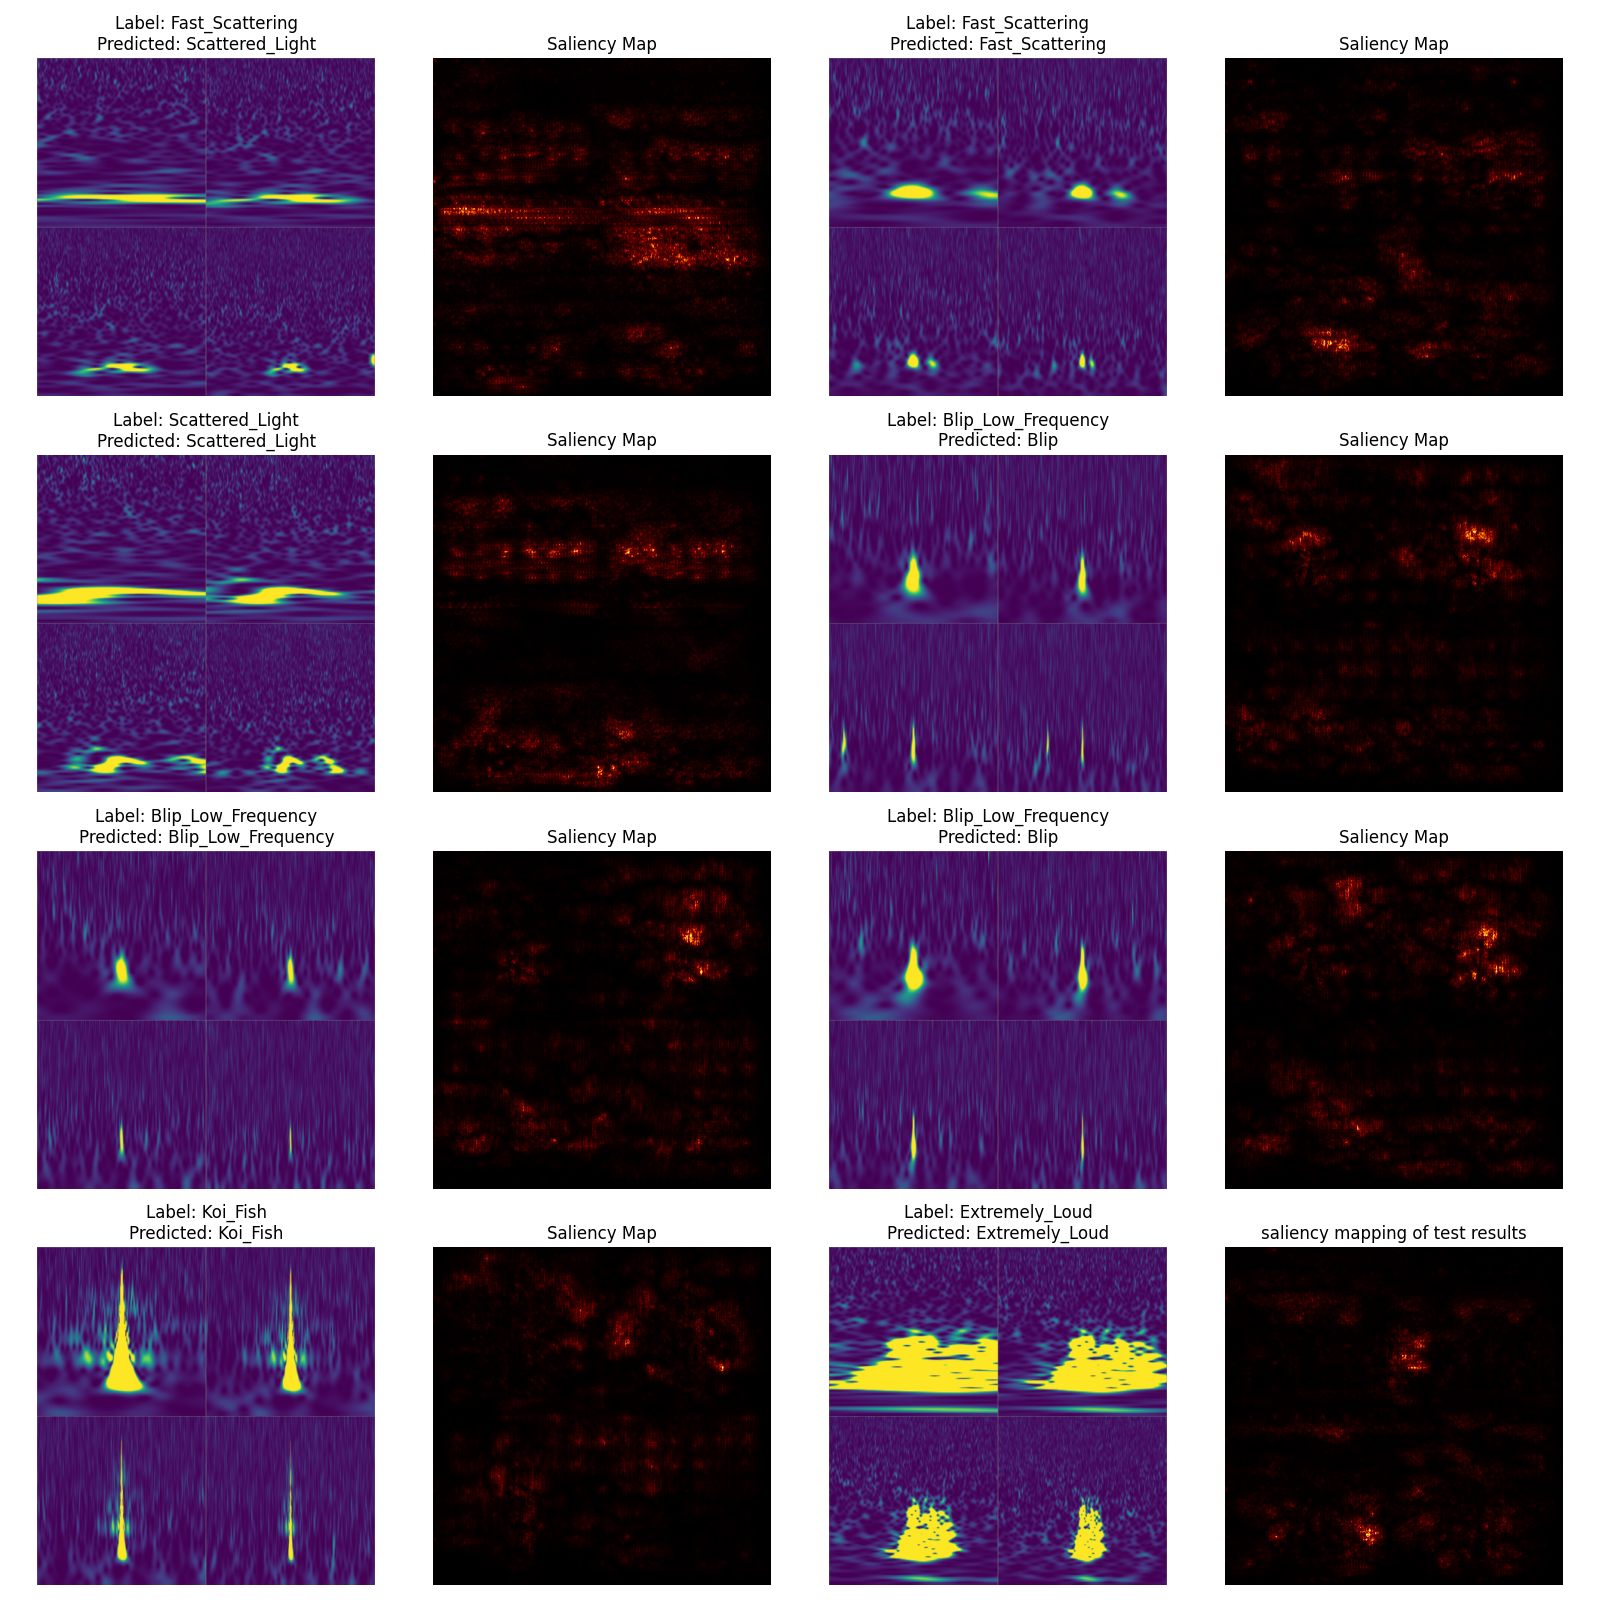
\includegraphics[width=0.95\textwidth]{Grad Assignment/Images/SaliencyMapping_Naive_MultiView_100epochs.png}
    \caption{Saliency Mapping of Naive baseline}
    \label{fig:saliency_naive_baseline}
\end{figure}

\newpage
\subsubsection{LwF strategy}
\label{subsubsec:RQ1_LWF}
A first \acrshort{cl} strategy addressing catastrophic forgetting is called \acrfull{lwf}. The model is trained, just as in the naive baseline, on five distinct tasks containing two classes per experience. 
The hyperparameter choices are: 
\begin{itemize}
    \item \verb|alpha=0.25|: $\alpha$ controls the balance between the loss on the new task and the distillation loss used to retain knowledge from old tasks. A value of 0.25 is a common choice based on the paper by \citep{oren2021defense}. 
    \item \verb|temperature=2.0|: $\tau$ controls the "softness" of the logits during knowledge distillation. A higher $\tau$ leads to softer targets, encouraging the network to learn a more generalizable presentation that benefits both old and new tasks. 
\end{itemize}

The strategy is augmented with the same \verb|ReplayPlugin|. 
Early stopping is not inherently supported by \acrshort{lwf} and thus not applied. 

The weight distribution changes are tracked as well. A similar behavior can be found. For illustrative purposes we only show the violin plots after the first and the last experience. 

\begin{figure}[ht]
\centering
\begin{subfigure}
  \centering
  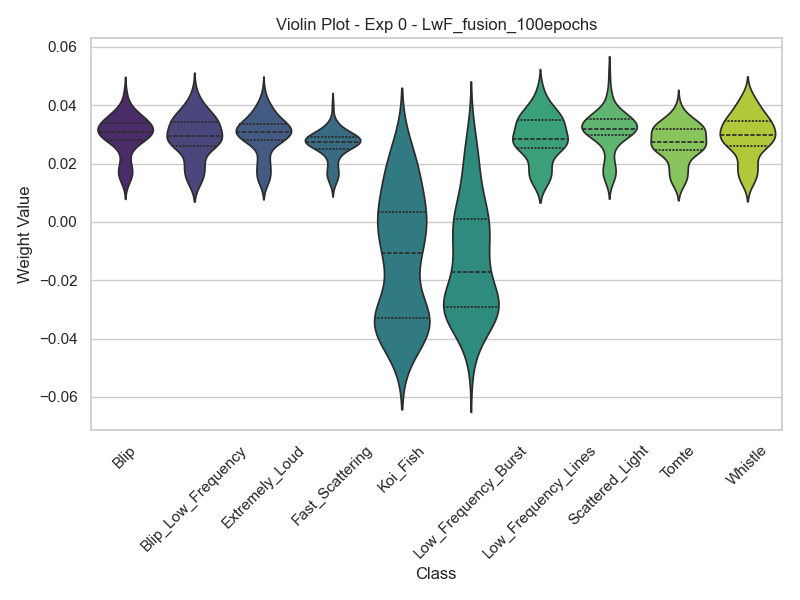
\includegraphics[width=0.4\textwidth]{Grad Assignment/Images/LwF_fusion_100epochs_exp_0.png}  
  \label{fig:lwf_violin_exp_0}
\end{subfigure}
\begin{subfigure}
  \centering
  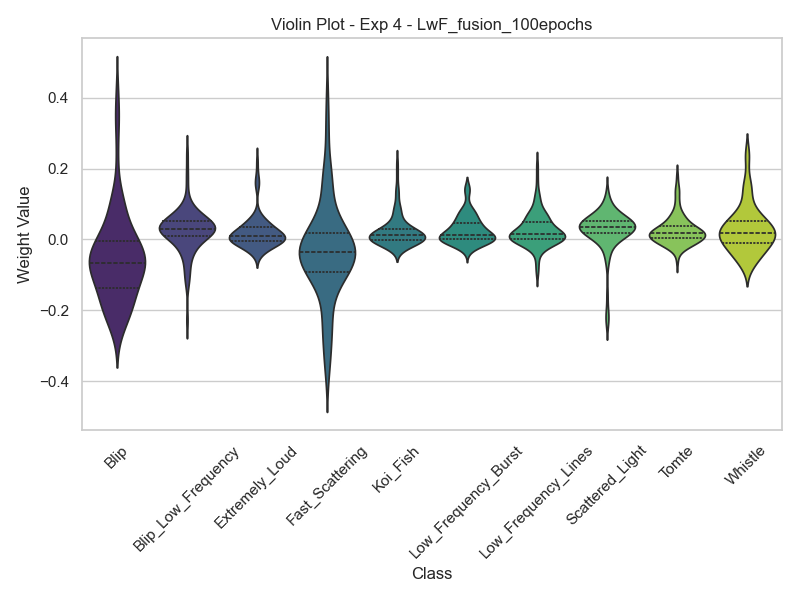
\includegraphics[width=0.4\textwidth]{Grad Assignment/Images/LwF_fusion_100epochs_exp_4.png}  
  \label{fig:lwf_violin_exp_4}
\end{subfigure}
\caption{Weight distribution changes}
\label{fig:lwf_weight_distribution}
\end{figure}

From the Confusion Matrix, f1 plot and Classification report as shown in Figure \ref{fig:cm_f1_lwf_baseline} and Table \ref{tbl:RQ1_class_report_LWF} we find that the overall accuracy is $88.2 \%$, higher than the naive baseline. But 'Blip\_Low\_Frequency' and 'Tomte' still suffer from a lot of False Negatives, on the other hand 'Blip' suffers from a lot of False Positives. 

\begin{figure}[ht]
\centering
\begin{subfigure}
  \centering
  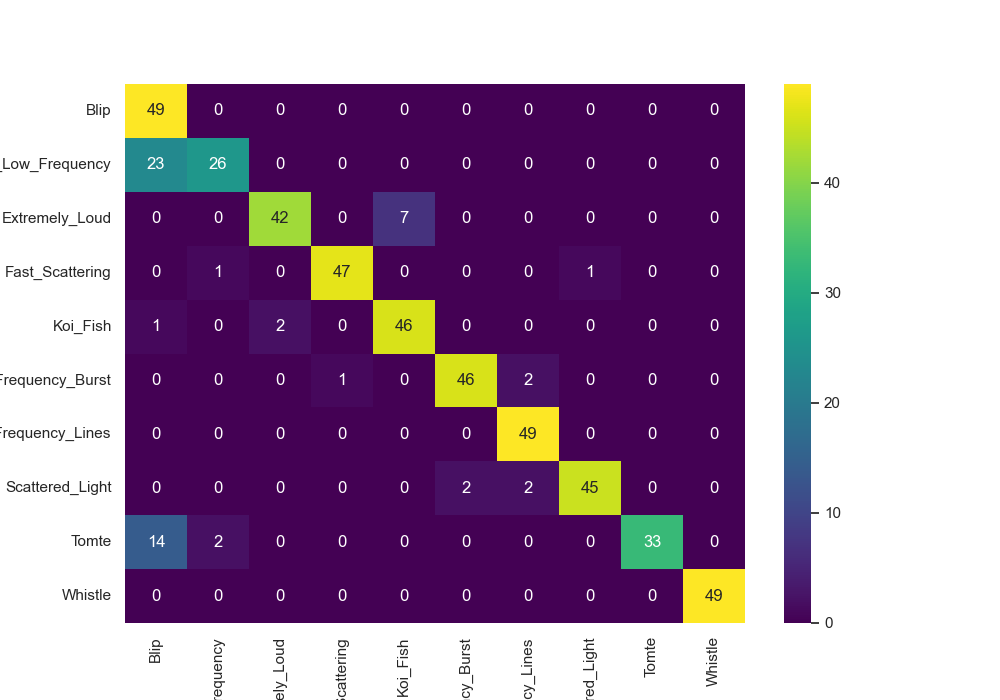
\includegraphics[width=0.49\textwidth]{Images/cm_LwF_MultiView_100epochs.png}  
  \label{fig:sub-first}
\end{subfigure}
\begin{subfigure}
  \centering
  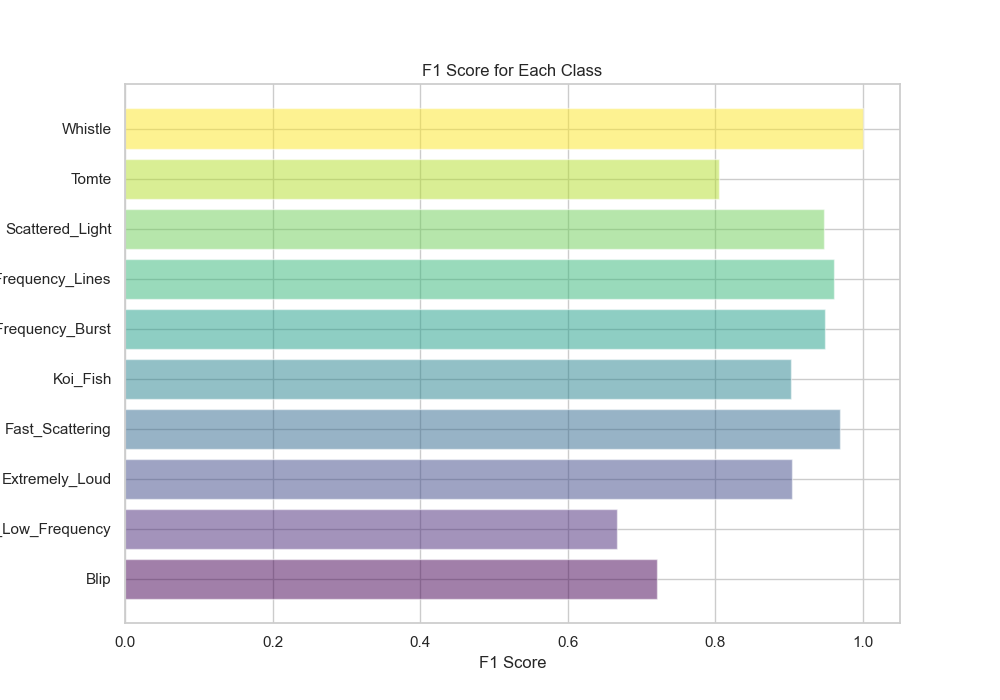
\includegraphics[width=0.49\textwidth]{Images/f1_LwF_MultiView_100epochs.png}  
  \label{fig:sub-second}
\end{subfigure}
\caption{Confusion matrix and f1 plot for LwF strategy}
\label{fig:cm_f1_lwf_baseline}
\end{figure}

\begin{table}
\centering
    \begin{tabular}{|l|c c c|}
    \hline
    \textbf{Glitch type} & \textbf{Precision} & \textbf{Recall} & \textbf{f1-score} \\ \hline
    Blip & $0.56$ & $1.00$ & $0.72$ \\
    Blip\_Low\_Frequency & $0.90$ & $0.53$ & $0.67$\\
    Extremely\_Loud & $0.95$ & $0.86$ &  $0.90$\\
    Fast\_Scattering & $0.98$ & $0.96$ &  $0.97$\\
    Koi\_Fish & $0.87$ & $0.94$ & $0.90$\\
    Low\_Frequency\_Burst & $0.96$ & $0.94$ & $0.95$\\
    Low\_Frequency\_Lines & $0.92$ & $1.00$ & $0.96$\\
    Scattered\_Light & $0.98$ & $0.92$ &$0.95$ \\
    Tomte & $1.00$ & $0.67$ &$0.80$ \\
    Whistle & $1.00$ & $1.00$ & $1.00$ \\
    \hline
    \end{tabular}
    \caption{Classification report of the LwF strategy.}
    \label{tbl:RQ1_class_report_LWF}
\end{table}


Due to these findings, further exploration of the embedding using \acrshort{tsne} and \acrshort{umap} plots (in two dimensions) is necessary.\\ The \acrshort{tsne} and \acrshort{umap} representation, as shown in Figure \ref{fig:tSNE_LwF}, demonstrate a clustering of glitch categories in 2D space.


\begin{figure}[ht]
\centering
    \centering
    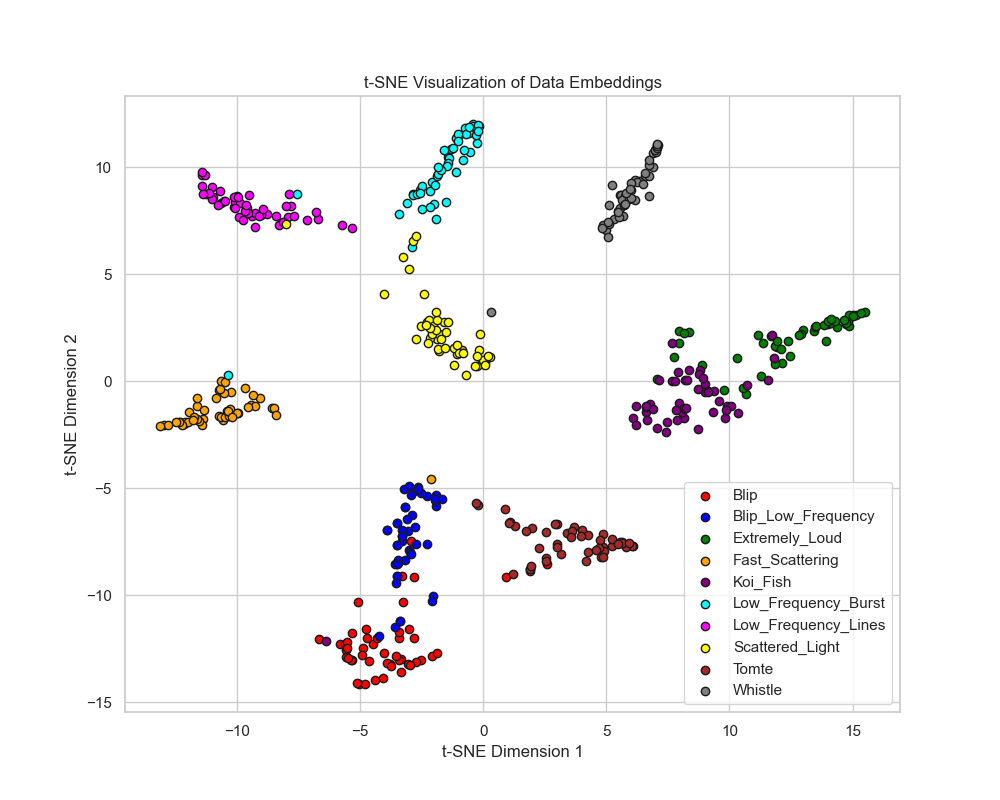
\includegraphics[width=0.6\textwidth]{Images/tSNE_LwF_MultiView_testset_100epochs.png}
    \caption{t-SNE visualization LwF}
    \label{fig:tSNE_LwF}
\end{figure}

\begin{figure}[ht]
  \centering
    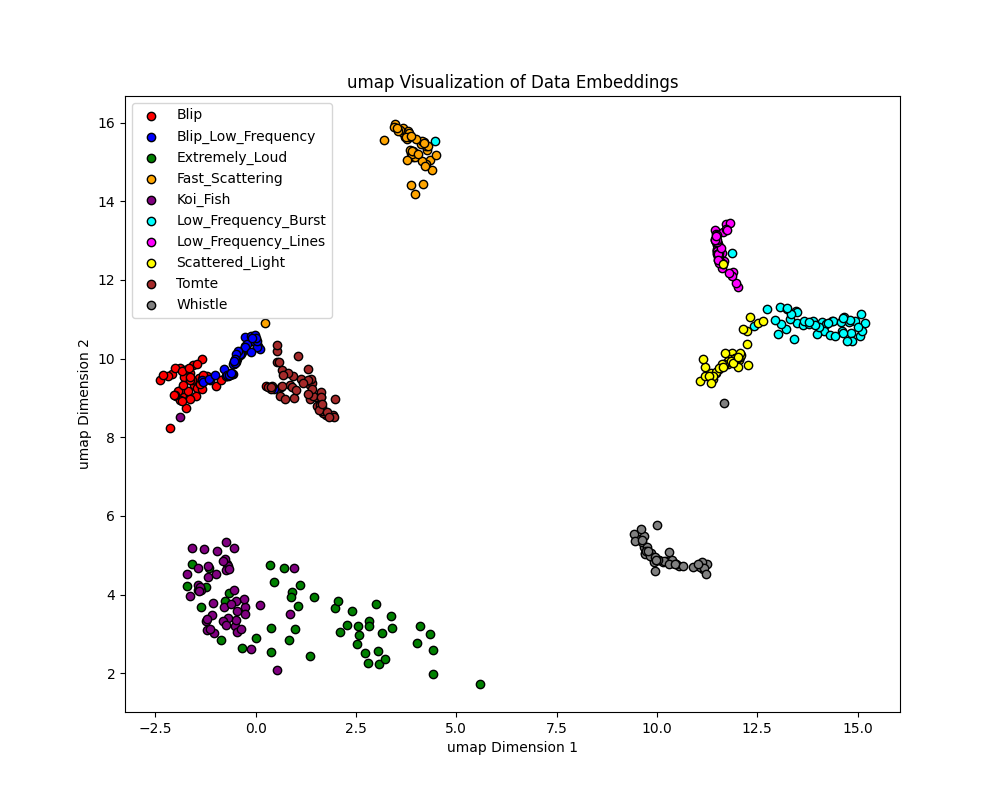
\includegraphics[width=0.6\textwidth]{Images/umap_MultiView_LwF_testset_100epochs.png}
    \caption{UMAP visualization LwF}
    \label{fig:umap_LwF}
\end{figure}


Some relevant observations that can be made: 
\begin{itemize}
    \item There seems to be a rough separation between glitches along t-SNE dimension 1. This is visible in both the t-SNE and UMAP visualization.  
    \item Potential similarities among certain glitch classes like "Koi\_Fish" and "Tomte" appear close together in the plot. This indicates that these classes share some underlying features. 
\end{itemize}

The images of the Saliency Mapping in Figure \ref{fig:saliency_lwf} show that the model attends to different regions of the spectrogram to classify different glitch types. The model makes a mistake in the top left image. This is predicted to be a 'Blip', but actually this is a 'Tomte'. 
When investigating the 'Koi\_Fish' pattern next to the 'Blip' and 'Tomte', we see that similar features are retrieved. This confirms the observations made by the t-SNE and UMAP visualizations. 

\begin{figure}[ht]
    \centering
    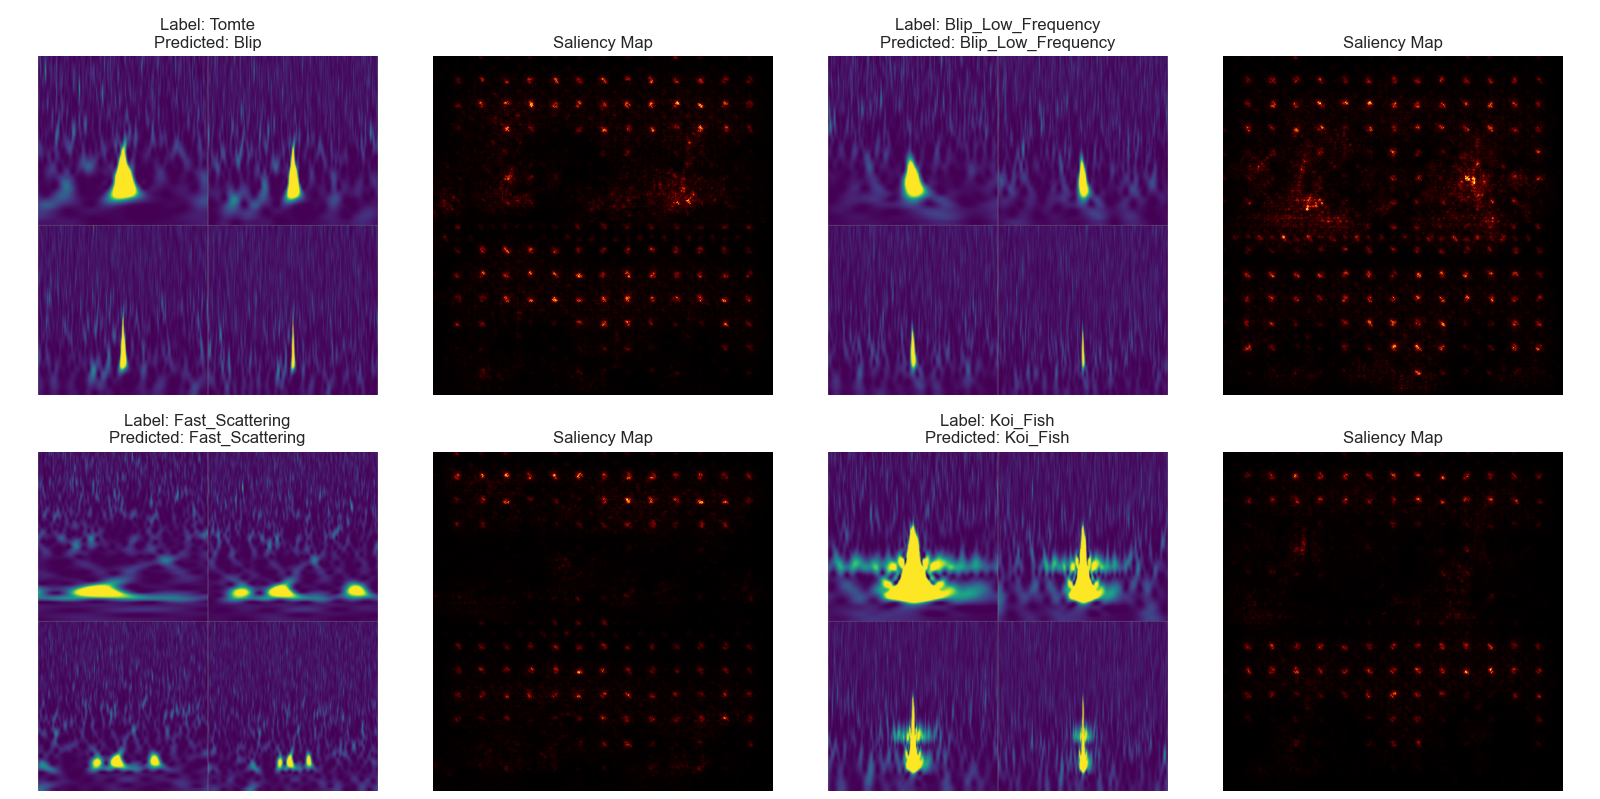
\includegraphics[width=0.95\textwidth]{Images/SaliencyMapping_LwF_MultiView_100epochs_selection.png}
    \caption{Saliency Mapping of LwF}
    \label{fig:saliency_lwf}
\end{figure}

\newpage

\subsubsection{AGEM strategy}
\label{subsubsec:RQ1_AGEM}
A second \acrshort{cl} strategy addressing catastrophic forgetting is called \acrfull{agem}. \acrshort{agem} utilises an episodic memory of gradients computed on past tasks. During training, it computes the gradient of the current model with respect to the new task's loss. It then compares the gradient with the average gradient computed on the past tasks. If the new gradient deviates significantly from the average, \acrshort{agem} adjusts the update direction to prevent catastrophic forgetting. The model is trained, just as in the naive baseline, on five distinct tasks that contain two classes per experience. 

The strategy is augmented with the \verb|ReplayPlugin| used in the previous strategy, but also an \verb|AGEMPlugin|. The \verb|AGEMPlugin| is specifically designed for \acrshort{agem} it maintains a set of past examples. 

The hyperparameter choices are: 
\begin{itemize}
    \item \verb|patterns_per_exp|: The number of patterns (samples) stored for each past experience. Based on the papers by \citep{chaudhry2018efficient, lopez2017gradient} and the fact there are 10 patterns in the benchmark, here we opt for a value of '10'. 
    \item \verb|sample_size|: The number of patterns sampled from the memory buffer during training. Here we opt for the default same sample size equal to the dataloader batch size. 
\end{itemize}


Changes in weight distribution are tracked for illustrative purposes and shown in Figure \ref{fig:agem_weight_distribution}

\begin{figure}[ht]
\centering
\begin{subfigure}
  \centering
  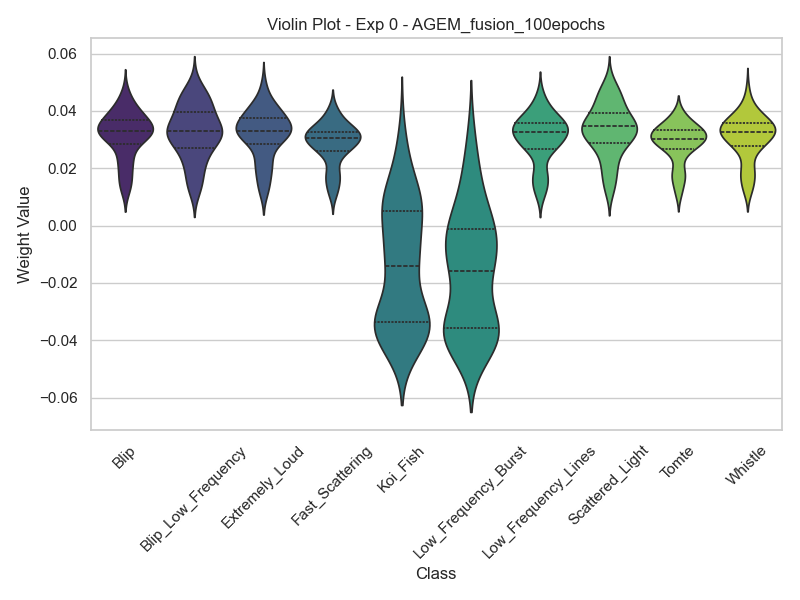
\includegraphics[width=0.4\textwidth]{Grad Assignment/Images/AGEM_fusion_100epochs_exp_0.png}  
  \label{fig:agem_violin_exp_0}
\end{subfigure}
\begin{subfigure}
  \centering
  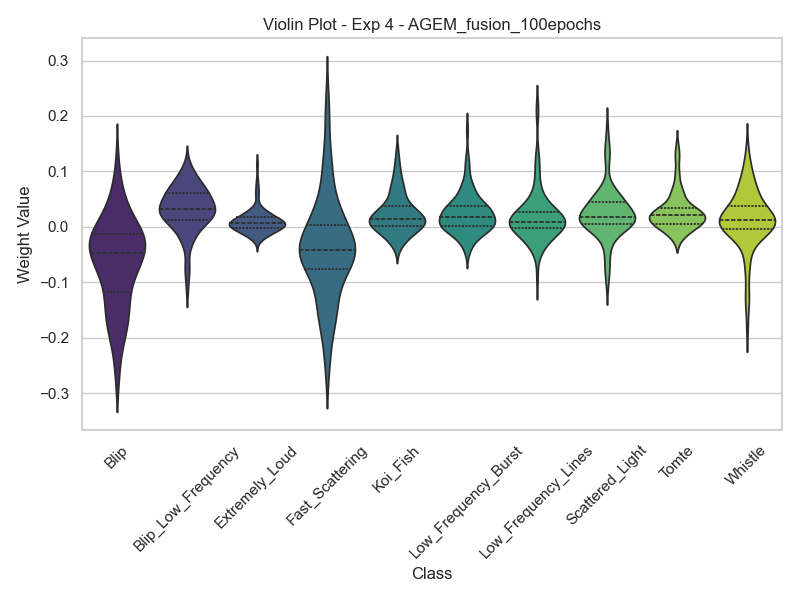
\includegraphics[width=0.4\textwidth]{Grad Assignment/Images/AGEM_fusion_100epochs_exp_4.png}  
  \label{fig:agem_violin_exp_4}
\end{subfigure}
\caption{Weight distribution changes}
\label{fig:agem_weight_distribution}
\end{figure}

From the Confusion Matrix, f1 plot and Classification report as shown in Figure \ref{fig:cm_f1_agem_baseline} and Table \ref{tbl:RQ1_class_report_agem} we find that the overall accuracy is $87 \%$, one percent point lower than the LwF results as depicted in \ref{subsubsec:RQ1_LWF}. The model performs well on the majority of classes, but struggles with 'Tomte' and 'Blip\_Low\_Frequency'. Especially the recall on 'Tomte' is very low, indicating a high number of False Negatives. On the other hand, if the 'Tomte' glitch class is detected, the model is very reliable (high precision). 

\begin{figure}[H]
\centering
\begin{subfigure}
  \centering
  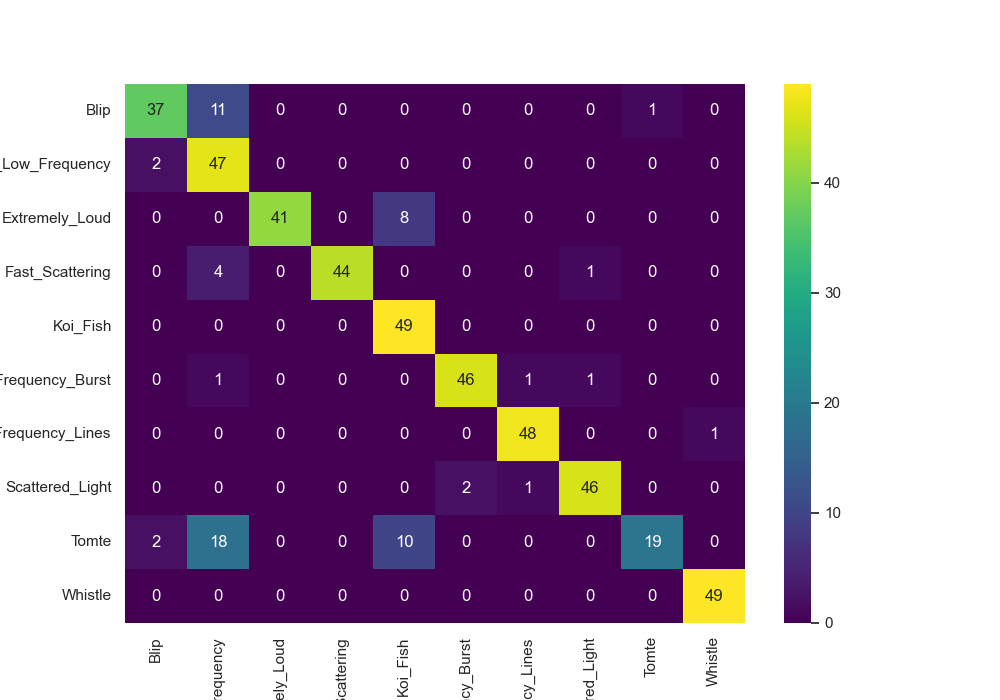
\includegraphics[width=0.49\textwidth]{Images/cm_AGEM_MultiView_100epochs.png}  
  \label{fig:sub-first}
\end{subfigure}
\begin{subfigure}
  \centering
  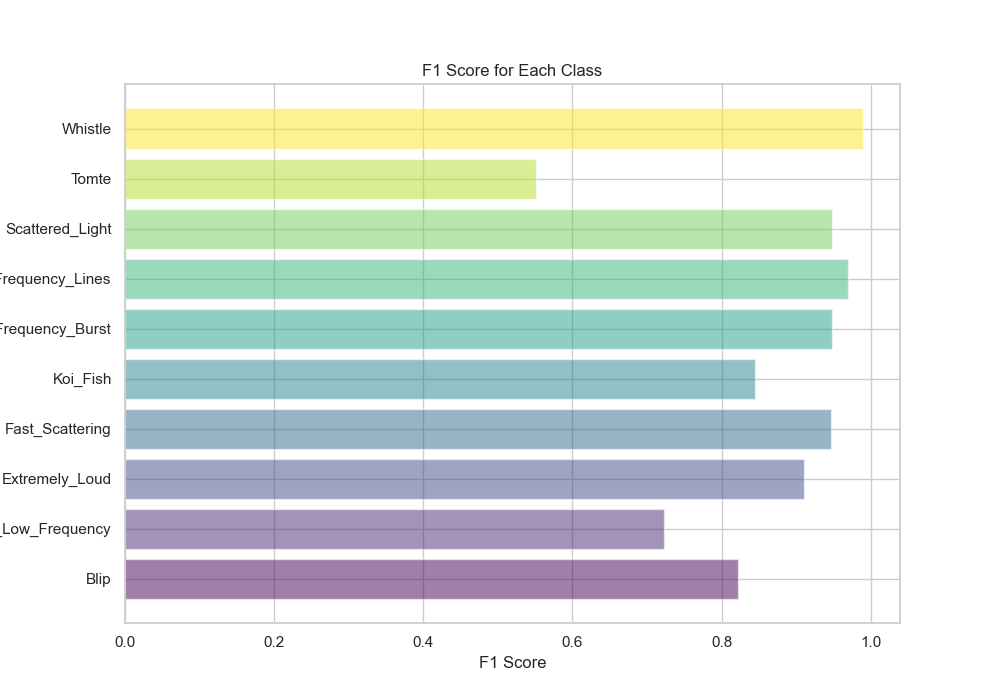
\includegraphics[width=0.49\textwidth]{Grad Assignment/Images/f1_AGEM_MultiView_100epochs.png}  
  \label{fig:sub-second}
\end{subfigure}
\caption{Confusion matrix and f1 plot for AGEM strategy}
\label{fig:cm_f1_agem_baseline}
\end{figure}

\begin{table}
\centering

    \begin{tabular}{|l|c c c|}
    \hline
    \textbf{Glitch type} & \textbf{Precision} & \textbf{Recall} & \textbf{f1-score} \\ \hline
    Blip & $0.90$ & $0.76$ & $0.82$ \\
    Blip\_Low\_Frequency & $0.58$ & $0.96$ & $0.72$\\
    Extremely\_Loud & $0.1.00$ & $0.84$ &  $0.91$\\
    Fast\_Scattering & $1.00$ & $0.90$ &  $0.95$\\
    Koi\_Fish & $0.73$ & $1.00$ & $0.84$\\
    Low\_Frequency\_Burst & $0.96$ & $0.94$ & $0.95$\\
    Low\_Frequency\_Lines & $0.96$ & $0.98$ & $0.97$\\
    Scattered\_Light & $0.96$ & $0.94$ &$0.95$ \\
    Tomte & $0.95$ & $0.39$ &$0.55$ \\
    Whistle & $0.98$ & $1.00$ & $0.99$ \\
    \hline
    \end{tabular}
    \caption{Classification report of the AGEM strategy.}
    \label{tbl:RQ1_class_report_agem}
\end{table}

Similar findings can be found from the investigation of the embedding space using \acrshort{tsne} and \acrshort{umap} plots in Figure \ref{fig:tsne_umap_AGEM},.

\begin{figure}[ht]
\centering
\begin{subfigure}
    \centering
    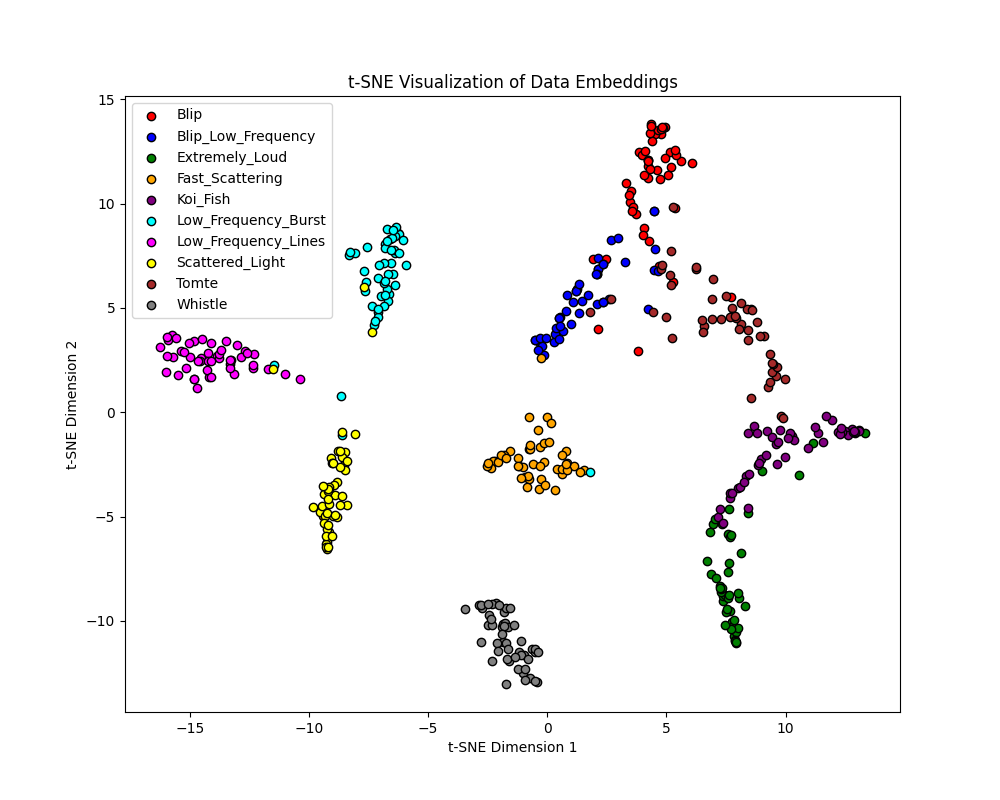
\includegraphics[width=0.45\textwidth]{Images/tSNE_AGEM_MultiView_testset_100epochs.png}
\end{subfigure}
\begin{subfigure}
    \centering
    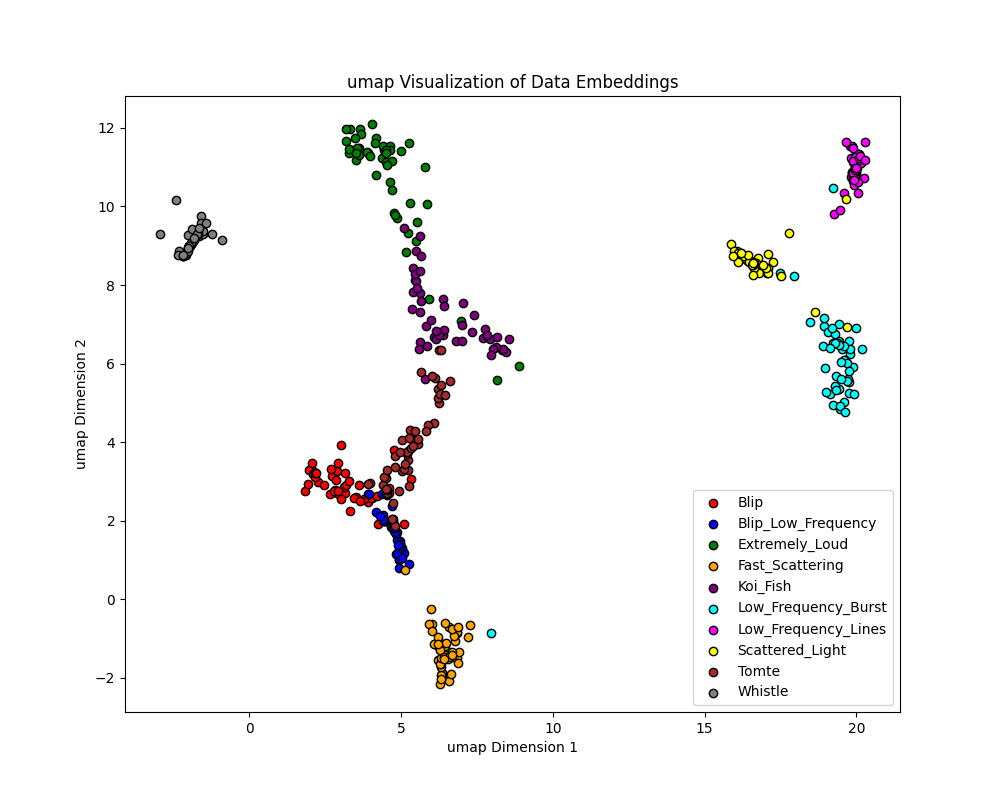
\includegraphics[width=0.45\textwidth]{Images/umap_MultiView_AGEM_testset_100epochs.png}
\end{subfigure}
    \caption{t-SNE and UMAP visualisation of the AGEM strategy.}
    \label{fig:tsne_umap_AGEM}
\end{figure}
Example saliency mappings can be found in Appendix \ref{appendix4}.  
\newpage

\subsubsection{EWC strategy}
\label{subsubsec:RQ1_EWC}
A third \acrshort{cl} strategy addressing catastrophic forgetting is called \acrfull{ewc}. \acrshort{ewc} acts like a memory preserver in neural networks. During training on new experiences, \acrshort{ewc} penalizes large updates to important weights used in previous tasks. This gentles the learning process, allowing the network to adapt to new information while retaining previously learned knowledge, hence avoiding recency bias. \\


The strategy is augmented with the \verb|ReplayPlugin| used in the previous strategies. An extra hyperparameter, \verb|ewc_lambda|, must be selected. We choose a value of $\lambda = 0.1$, signifying a moderate penalty for weight updates when training on new tasks. Typically, a greater value (approaching 1) emphasizes the preservation of previous knowledge, although it may hinder the acquisition of new skills.

\begin{figure}[H]
\centering
\begin{subfigure}
  \centering
  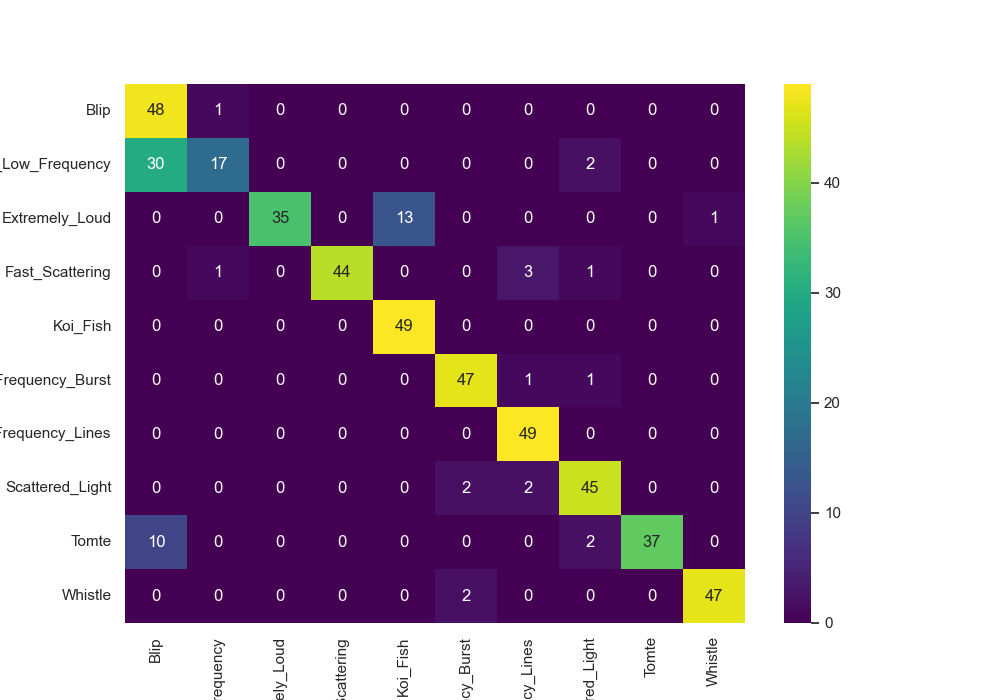
\includegraphics[width=0.49\textwidth]{Images/cm_EWC_MultiView_100epochs.png}  
  \label{fig:sub-first}
\end{subfigure}
\begin{subfigure}
  \centering
  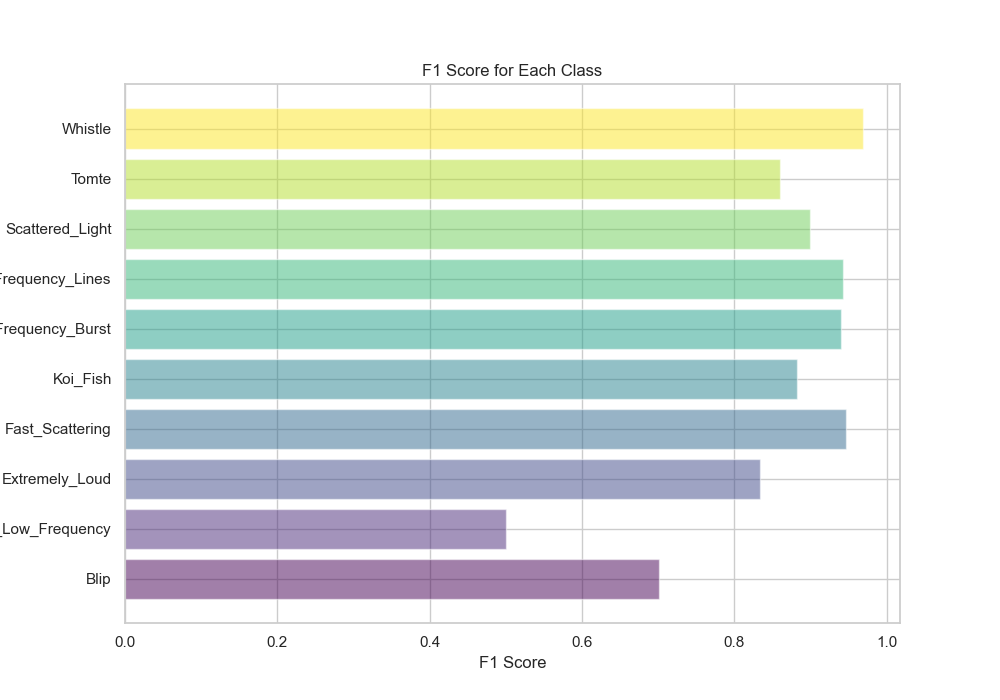
\includegraphics[width=0.49\textwidth]{Images/f1_EWC_MultiView_100epochs.png}  
  \label{fig:sub-second}
\end{subfigure}
\caption{Confusion matrix and f1 plot for EWC strategy}
\label{fig:cm_f1_ewc_baseline}
\end{figure}

\begin{table}[ht]
\centering
    \begin{tabular}{|l|c c c|}
    \hline
    \textbf{Glitch type} & \textbf{Precision} & \textbf{Recall} & \textbf{f1-score} \\ \hline
    Blip & $0.55$ & $0.98$ & $0.70$ \\
    Blip\_Low\_Frequency & $0.89$ & $0.35$ & $0.50$\\
    Extremely\_Loud & $1.00$ & $0.71$ &  $0.83$\\
    Fast\_Scattering & $1.00$ & $0.90$ &  $0.95$\\
    Koi\_Fish & $0.79$ & $1.00$ & $0.88$\\
    Low\_Frequency\_Burst & $0.92$ & $0.96$ & $0.94$\\
    Low\_Frequency\_Lines & $0.89$ & $1.00$ & $0.94$\\
    Scattered\_Light & $0.88$ & $0.92$ &$0.90$ \\
    Tomte & $1.00$ & $0.76$ & $0.86$ \\
    Whistle & $0.98$ & $0.96$ & $0.97$ \\
    \hline
    \end{tabular}
    \caption{Classification report of the EWC strategy.}
    \label{tbl:RQ1_class_report_ewc}
\end{table}


From the Confusion Matrix, f1 plot and Classification report as shown in Figure \ref{fig:cm_f1_ewc_baseline} and Table \ref{tbl:RQ1_class_report_ewc} we find that the overall accuracy is $85 \%$, several percent points lower than the previous best LwF results as depicted in \ref{subsubsec:RQ1_LWF}. The model performs well on the majority of classes, but struggles with 'Blip' and 'Blip\_Low\_Frequency'. Especially the recall on 'Blip\_Low\_Frequency' is very low.

\newpage
\subsubsection{DER strategy}
\label{subsubsec:RQ1_DER}
\acrfull{der} combats recency bias by replaying past predictions, acting like a teacher. It stores the model's past outputs (logits) from old tasks alongside the original data. During training on new experiences (new classes), \acrshort{der} forces the model's current predictions on old data to align with its past predictions, reminding it of what it already knew, thus hindering catastrophic forgetting. \\
The hyperparameter \verb|alpha| controls the weight given to the replay loss (from past predictions) compared to the current task loss. A value of $\alpha = 1.0$ means that the replay loss is given equal importance to the current task loss during training on new experiences. Basically the model must optimize two things equally: 1) Fitting the new data and 2) Staying consistent with past predictions \citep{buzzega2020dark}.
\begin{figure}[H]
\centering
\begin{subfigure}
  \centering
  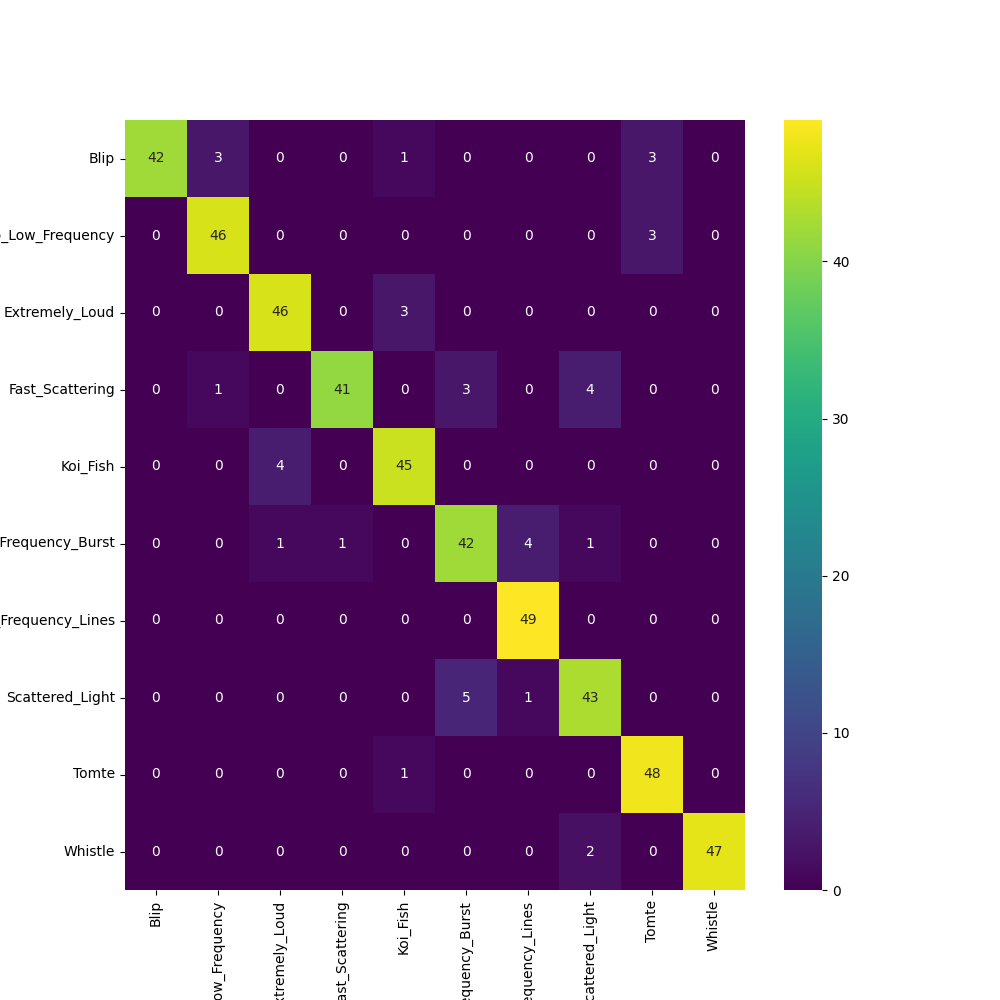
\includegraphics[width=0.49\textwidth]{Images/cm_DER_MultiView_100epochs.png}  
  \label{fig:sub-first}
\end{subfigure}
\begin{subfigure}
  \centering
  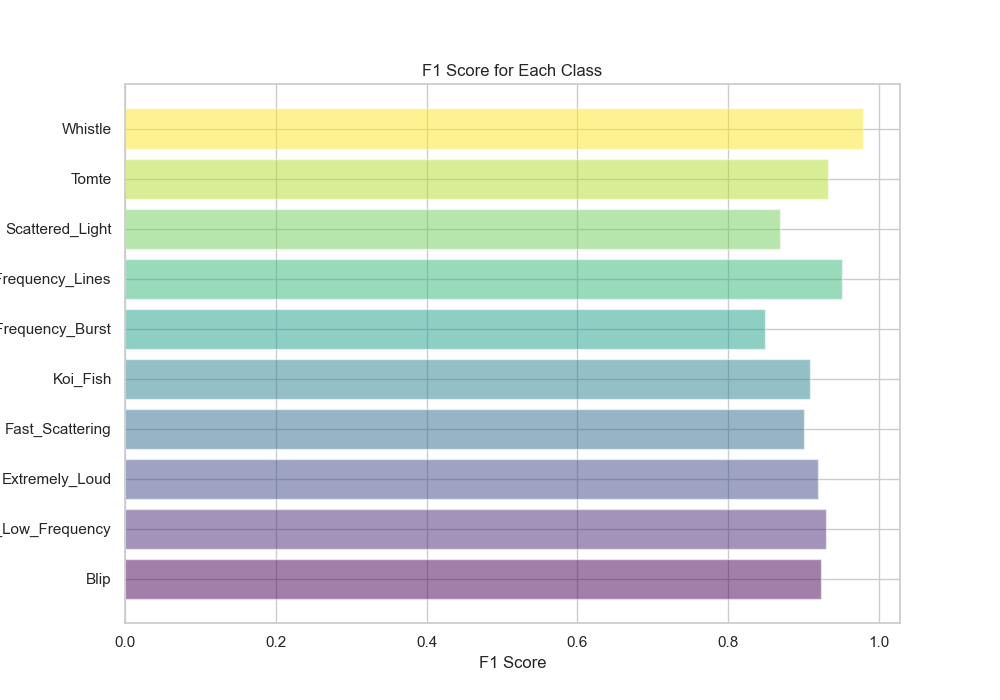
\includegraphics[width=0.49\textwidth]{Images/f1_DER_MultiView_100epochs.png}  
  \label{fig:sub-second}
\end{subfigure}
\caption{Confusion matrix and f1 plot for DER strategy}
\label{fig:cm_f1_der_baseline}
\end{figure}
\begin{table}[ht]
\centering
    \begin{tabular}{|l|c c c|}
    \hline
    \textbf{Glitch type} & \textbf{Precision} & \textbf{Recall} & \textbf{f1-score} \\ \hline
    Blip & $1.00$ & $0.86$ & $0.92$ \\
    Blip\_Low\_Frequency & $0.92$ & $0.94$ & $0.93$\\
    Extremely\_Loud & $0.90$ & $0.94$ &  $0.92$\\
    Fast\_Scattering & $0.98$ & $0.84$ &  $0.90$\\
    Koi\_Fish & $0.90$ & $0.92$ & $0.91$\\
    Low\_Frequency\_Burst & $0.84$ & $0.86$ & $0.85$\\
    Low\_Frequency\_Lines & $0.91$ & $1.00$ & $0.95$\\
    Scattered\_Light & $0.86$ & $0.88$ &$0.87$ \\
    Tomte & $0.89$ & $0.98$ & $0.93$ \\
    Whistle & $1.00$ & $0.96$ & $0.98$ \\
    \hline
    \end{tabular}
    \caption{Classification report of the DER strategy.}
    \label{tbl:RQ1_class_report_der}
\end{table}

From the Confusion Matrix, f1 plot and Classification report as shown in Figure \ref{fig:cm_f1_der_baseline} and Table \ref{tbl:RQ1_class_report_der} we find that the overall accuracy is $92\%$, more than the previous best \acrshort{lwf} strategy from \ref{subsubsec:RQ1_LWF}.\\

Because of the good results, it is noteworthy to further investigate the \acrshort{tsne} and \acrshort{umap} visualisations in Figure \ref{fig:tsne_umap_der}. 


\begin{figure}[ht]
\centering
\begin{subfigure}
    \centering
    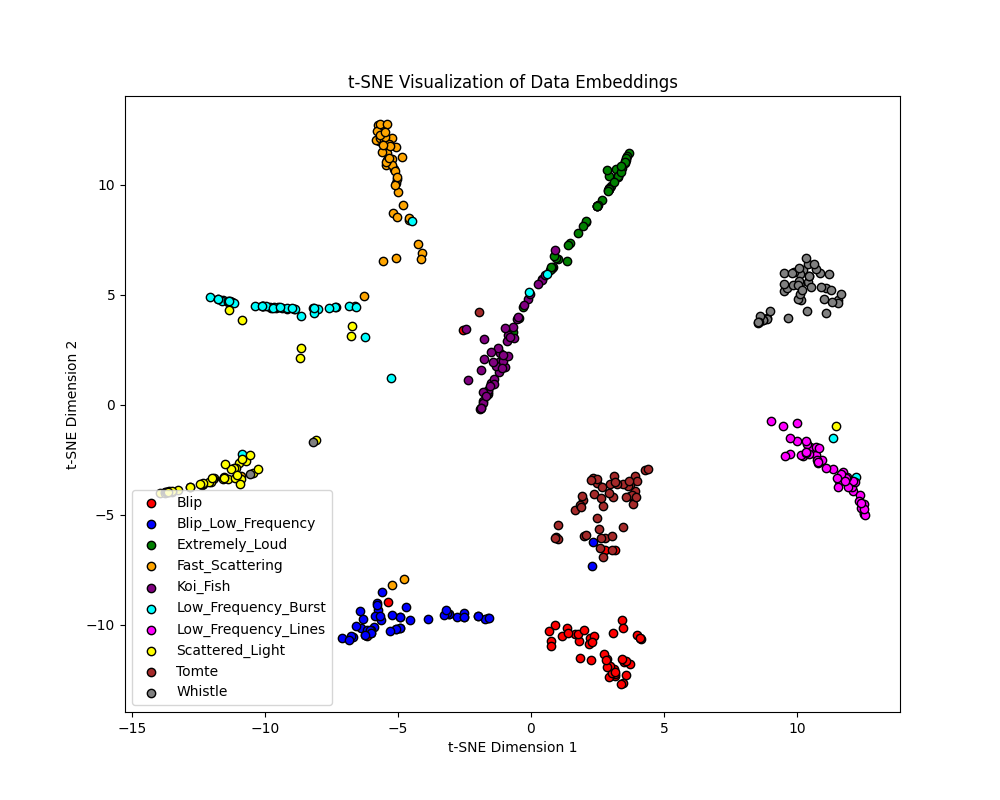
\includegraphics[width=0.45\textwidth]{Images/tSNE_DER_MultiView_testset_100epochs.png}
\end{subfigure}
\begin{subfigure}
    \centering
    \includegraphics[width=0.45\textwidth]{Images/umap_MultiView_DER_testset_100epochs.png}
\end{subfigure}
    \caption{t-SNE and UMAP visualisation of the DER strategy.}
    \label{fig:tsne_umap_der}
\end{figure}

Some relevant observations that can be made: 
\begin{itemize}
    \item The separation between 'Blip', 'Blip\_Low\_Frequency' and 'Tomte' is more defined as opposed to the previous best results. 
    \item \acrshort{der} seems to have more troubles with distinguishing 'Extremely\_Loud' and 'Koi\_Fish' glitch types. 
\end{itemize}

The images of the Saliency Mapping in Figure \ref{fig:saliency_der} visualise the above made observations more clearly. 

\begin{figure}[ht]
    \centering
    \includegraphics[width=0.95\textwidth]{Grad Assignment/Images/SaliencyMapping_DER_MultiView_100epochs_selection.png}
    \caption{Saliency Mapping of DER}
    \label{fig:saliency_der}
\end{figure}
\newpage

\subsubsection{DER++ strategy}
\label{subsubsec:RQ1_DER++}
\acrfull{der++} is an advanced version of \acrshort{der} from \ref{subsubsec:RQ1_DER}. It extends the replay buffer by also storing the ground truth logits and replay examples \citep{buzzega2020dark}. \acrshort{der++} mitigates, in this way, the shortcoming of \acrshort{der} that weakens when the logits are highly biased due to a sudden distribution shift \citep{ling2022difficulty}. 

\begin{figure}[H]
\centering
\begin{subfigure}
  \centering
  \includegraphics[width=0.49\textwidth]{Images/cm_DER++_MultiView_100epochs.png}  
  \label{fig:sub-first}
\end{subfigure}
\begin{subfigure}
  \centering
  \includegraphics[width=0.49\textwidth]{Images/f1_DER++_MultiView_100epochs.png}  
  \label{fig:sub-second}
\end{subfigure}
\caption{Confusion matrix and f1 plot for DER++ strategy}
\label{fig:cm_f1_der++_baseline}
\end{figure}
\begin{table}[ht]
\centering
    \begin{tabular}{|l|c c c|}
    \hline
    \textbf{Glitch type} & \textbf{Precision} & \textbf{Recall} & \textbf{f1-score} \\ \hline
    Blip & $0.80$ & $0.96$ & $0.87$ \\
    Blip\_Low\_Frequency & $0.90$ & $0.92$ & $0.91$\\
    Extremely\_Loud & $0.97$ & $0.69$ &  $0.81$\\
    Fast\_Scattering & $0.98$ & $0.92$ &  $0.95$\\
    Koi\_Fish & $0.75$ & $0.98$ & $0.85$\\
    Low\_Frequency\_Burst & $0.92$ & $0.92$ & $0.92$\\
    Low\_Frequency\_Lines & $0.92$ & $1.00$ & $0.96$\\
    Scattered\_Light & $0.96$ & $0.92$ & $0.94$ \\
    Tomte & $1.00$ & $0.78$ & $0.87$ \\
    Whistle & $1.00$ & $1.00$ & $1.00$ \\
    \hline
    \end{tabular}
    \caption{Classification report of the DER++ strategy.}
    \label{tbl:RQ1_class_report_der++}
\end{table}

From the Confusion Matrix, f1 plot and Classification report as shown in Figure \ref{fig:cm_f1_der++_baseline} and Table \ref{tbl:RQ1_class_report_der++} we find that the overall accuracy is $91\%$, one percent point less than the previous best \acrshort{der} strategy from \ref{subsubsec:RQ1_DER}. It has perfect results on 'Whistle' glitches. \\

\newpage
\subsubsection{SCR strategy}
As described in \ref{sec:SCR}, \acrshort{scr} leverages the Nearest-Class-Mean classifier as a substitute for the Softmax classifier by addressing recency bias and avoiding structural changes in the fully-connected layer for new classes. There is however a risk involved, the effectiveness of \acrshort{scr} might depend on the quality of the data embeddings and the between-class separation. It also has the tendency of introducing additional bias \citep{mai2021supervised, aleixo2023catastrophic}.   



\subsection{RQ2}
\label{subsec:RQ2}
Each of the strategies are trained for 15 epochs on every task (of learning the weights on the three classes). More training epochs resulted in overfitting behavior. Between 10 and 15 epochs of training the results converge. The order in which the classes are fed is kept the same over all strategies (1 = \{Whistle\}, 2 = \{Scattered\_Light \}, 3 = \{Tomte \}).

\subsubsection{Naive CL strategy (baseline)}
As baseline we use the \acrshort{cl} stategy 'Naive', the hyperparameter choices and additional plugins are similar to those in \ref{subsubsec:RQ1_naive_baseline}. One difference, the benchmark consists of 3 experiences where each experience contains instances of 1 class only. 
During training we track the weight distribution changes via violin distribution plots. In the following table, \ref{tbl:naive_fd_weights}, the violin plots for the second and last experience are shown.
After the first 15 epochs training on differentiating the classes from experience 0 to 2 we get: 
\begin{center}
\begin{tabular}{cc}
\includegraphics[width=0.4\textwidth]{Images/naive_fd_exp_1.png} & \includegraphics[width=0.4\textwidth]{Images/naive_fd_exp_2.png} \\
\end{tabular}
\label{tbl:naive_fd_weights}
\end{center}

From the Confusion Matrix as shown in Figure \ref{fig:cm_f1_FD_naive_baseline}-(a) we find that the overall accuracy is $92,56 \%$. The model performs well on the 'Whistle' and 'Scattered\_Light' class, but struggles some more with 'Tomte'. The F1 scores for all of the classes are above 0.9, the lowest being the 'Tomte' result with $f1=0.90$, scores above 0.9 are considered very good. 

\begin{figure}[ht]
\centering
\begin{subfigure}
  \centering
  \includegraphics[width=0.45\textwidth]{Images/cm_FD_model_naive.png}  
  \label{fig:fd_sub-first}
\end{subfigure}
\begin{subfigure}
  \centering
  \includegraphics[width=0.50\textwidth]{Images/f1_FD_model_naive.png}  
  \label{fig:fd_sub-second}
\end{subfigure}
\caption{Confusion matrix and f1 plot for Naive baseline}
\label{fig:cm_f1_FD_naive_baseline}
\end{figure}

Just as in our experiments for \ref{subsec:RQ1} we investigate the \acrshort{tsne} and \acrshort{umap} representations. 
The t-SNE visualization as shown in Figure \ref{fig:tSNE_FD_Naive} illustrates the clustering of three glitch classes in 2D space. The three classes appear to be well-separated in the plot, which suggests that the model is able to effetively distinguish between these types of glitches. The density of the point clouds indicates the data samples within a class are very similar to eachother. There is, however, some overlap between 'Tomte' and the two other classes.\\

A similar interpretation can be made from Figure \ref{fig:umap_FD_Naive}. The 'Whistle' class forms a distinct elongated cluster. This suggests that the instances are relatively similar to eachother in the high-dimensional space. The 'Tomte' cluster is a compact group, but relatively close to other clusters. It is evident that there is overlap among different classes. This raises the concern whether some instances might have been incorrectly classified during manual labeling. 

\begin{figure}[ht]
\centering
\begin{subfigure}
  \centering
    \includegraphics[width=0.6\textwidth]{Grad Assignment/Images/tSNE_FractalDimension_naive_test.png}
    \caption{t-SNE visualization Naive FD strategy}
    \label{fig:tSNE_FD_Naive}
\end{subfigure}
\begin{subfigure}
  \centering
    \includegraphics[width=0.6\textwidth]{Grad Assignment/Images/umap_FractalDimension_naive_test.png}
    \caption{UMAP visualization Naive FD strategy}
    \label{fig:umap_FD_Naive}
\end{subfigure}
\end{figure}

%\input{Chapter5/chapter-5}

%\input{Chapter6/chapter-6}



\backmatter
\pagenumbering{roman}

\bibliographystyle{plainnat}
\bibliography{report}

%% Use letters for the chapter numbers of the appendices.
%\appendix
\appendix
  \chapter{MultiViewColorNet\_resnet18}
\label{appendix1}
\begin{verbatim}
class MultiViewColorNet_resnet18(nn.Module):
  def __init__(self, num_classes=10):
    # Call the parent class's constructor
    super(MultiViewColorNet_resnet18, self).__init__()
    # Initialize a pretrained ResNet-18 model with adjusted input size
    self.resnet = models.resnet18(weights='DEFAULT')
    # Access the first convolutional layer
    first_conv = self.resnet.conv1
    # Modify the kernel size of the first convolution
    first_conv.kernel_size = (7, 7)
    # Unfreeze all parameters in the model for training
    for param in self.resnet.parameters():
      param.requires_grad = True
    # Get the number of features in the last layer of the model
    num_features_in = self.resnet.fc.in_features
    # Replace the last layer with a new linear layer
    self.resnet.fc = nn.Linear(num_features_in, 120)
    # Add a second fully connected layer
    self.fc2 = nn.Linear(120, 84)
    # Add a third fully connected layer for the num_classes classes 
    in the GravitySpy dataset
    self.fc3 = nn.Linear(84, num_classes)
    # Add a dropout layer to prevent overfitting
    self.dropout = nn.Dropout(p=0.3)
    # Add a batch normalization layer
    self.bn = nn.BatchNorm1d(120)

  def forward(self, x):
    # Forward pass: compute the output of the model by passing 
    the input through the model
    x = self.resnet(x)
    # Apply batch normalization
    x = self.bn(x)
    # Apply the ReLU activation function
    x = F.relu(self.fc2(x))
    # Apply dropout
    x = self.dropout(x)
    # Pass the result through the final fully connected layer
    x = self.fc3(x)
    # Return the model's output
    return x
\end{verbatim}
  \chapter{MultiViewGravitySpyDataset DataLoader}
\label{appendix2}
\begin{verbatim}
class MultiViewGravitySpyDataset(ImageFolder):
    def __init__(self, root, cls, transform=None):
        self.data_dir = root
        self.classes = cls
        self.class_to_indx = {c: i for i, c in enumerate(self.classes)}
        self.image_paths = []
        self.labels = []
        self.versions = ["0.5.png", "1.0.png", "2.0.png", "4.0.png"]
        for class_name in self.classes:
            class_path = os.path.join(root, class_name)
            for filename in os.listdir(class_path):
              if any(filename.endswith(version) for version in self.versions):
                self.image_paths.append(os.path.join(class_path, filename))
                self.labels.append(self.class_to_indx[class_name])
        self.transform = transform

    def __len__(self):
        return len(self.image_paths) // 4  # Assuming 4 versions for each image

    def __getitem__(self, idx):
        image_paths = self.image_paths[idx*4: (idx+1)*4]  
        images = [Image.open(image_path).convert('RGB') for image_path 
        in image_paths]
        if self.transform:
            images = [self.transform(img) for img in images]
        top_row = Image.fromarray(np.concatenate([np.array(images[0]), 
        np.array(images[1])], axis=1))
        bottom_row = Image.fromarray(np.concatenate([np.array(images[2]), 
        np.array(images[3])], axis=1))
        final_image = Image.fromarray(np.concatenate([np.array(top_row), 
        np.array(bottom_row)], axis=0))
        temp = np.array(final_image) 
        temp = temp.astype(np.float32)
        temp /= 255.0
        fused_image = torch.from_numpy(temp.transpose((2, 0, 1)))
        label = self.labels[idx*4] 
        return fused_image, label
\end{verbatim}
  \begin{appendices}
\chapter{FractalDimensionConvNet}
\label{appendix3}
\begin{verbatim}
class FractalDimensionConvNet(nn.Module):
    def __init__(self):
        super(FractalDimensionConvNet, self).__init__()
        self.conv1 = nn.Conv1d(in_channels=50, out_channels=128, kernel_size=3, stride=1, padding=1) #adjust from 347 to 50
        self.bn1 = nn.BatchNorm1d(128)
        self.conv2 = nn.Conv1d(in_channels=128, out_channels=64, kernel_size=3, stride=1, padding=1)
        self.bn2 = nn.BatchNorm1d(64)
        self.conv3 = nn.Conv1d(in_channels=64, out_channels=32, kernel_size=3, stride=1, padding=1)
        self.bn3 = nn.BatchNorm1d(32)
        self.conv4 = nn.ConvTranspose1d(in_channels=32, out_channels=64, kernel_size=3, stride=1, padding=1)
        self.bn4 = nn.BatchNorm1d(64)
        self.fc1 = nn.Linear(64*56, 1024)
        #self.fc1 = nn.Linear(64*5, 1024) #adjust input size for fd statistics
        self.fc2 = nn.Linear(1024,256)
        self.dropout1 = nn.Dropout(0.1)
        self.dropout2 = nn.Dropout(0.3)
        self.fc3 = nn.Linear(256,3)

    def forward(self, x):
        x = nn.functional.selu(self.conv1(x))
        x = self.bn1(x)
        x = nn.functional.selu(self.conv2(x))
        x = self.bn2(x)
        x = nn.functional.selu(self.conv3(x))
        x = self.bn3(x)
        x = self.dropout1(x)
        x = nn.functional.selu(self.conv4(x))
        x = self.bn4(x)
        x = self.dropout2(x)
        x = x.view(x.size(0), -1)
        x = nn.functional.selu(self.fc1(x))
        x = nn.functional.relu(self.fc2(x))
        x = self.fc3(x)
        return x
\end{verbatim}
\end{appendices}
  
    \chapter{Saliency Mappings}
    \label{appendix4}


%  \input{Appendices/appendix-b}
%  \input{Appendices/appendix-c}


\end{document}
